\documentclass[a4paper,12pt,openright,twoside,titlepage]{report} 
% oneside - solo fronte, twoside - fronte retro
% openright - prima pagina dei capitoli su pagina destra, openany - indifferentement
\usepackage[bottom]{footmisc}
\usepackage{fancyhdr}
\usepackage{url}
\usepackage{latexsym}
\usepackage{amssymb}
\usepackage{amsfonts}                 %Pacchetto per inserire i caratteri matematici
\usepackage{makeidx}                  %Pacchetto per generare l'indice analitico
%\usepackage[utf8x]{inputenc}         %Pacchetto per poter inserire direttamente nel testo%lettere accentate. Se si scrive in inglese si può commentare
\usepackage[T1]{fontenc}              %Pacchetto che gestisce l'encoding T1
\usepackage[utf8]{inputenc}
\usepackage{textcomp}

\usepackage{lmodern}
\usepackage{bold-extra}
\normalfont %to load T1lmr.fd 
\DeclareFontShape{T1}{lmr}{bx}{sc} { <-> ssub * cmr/bx/sc }{}

\usepackage[english,italian]{babel}   %Pacchetto per la sillabazione delle parole in italiano e in inglese
%\usepackage[Sonny]{fncychap}         %Pacchetto per avere diversi tipi di titoli di capitolo diversi.  Commentare se si desidera avere i titoli in maniera normale. Gli stili possibili sono 2: Sonny, Lenny
\usepackage{enumitem}
\usepackage{verbatim}                 %Pacchetti per stampare il codice
\usepackage{listings}                 %Pacchetti per stampare il codice
\usepackage{fancyvrb}                 %Pacchetti per stampare il codice
\usepackage{algorithm}                %Pacchetti per stampare il codice	%Pacchetti per stampare il codice
\usepackage{algpseudocode}            %Pacchetti per stampare il codice
\usepackage[babel]{csquotes}
\usepackage{wrapfig}
\usepackage{epigraph}
\usepackage{acronym}
\usepackage{hyperref}
\usepackage{graphicx} %gestione immagini, anche vettoriali
\usepackage[outdir=./build/pdf_converted/]{epstopdf} %per utilizzare eps nel file
\usepackage[position=bottom]{subfig}
\usepackage[style=authoryear,sorting=nyt,maxcitenames=1,backend=bibtexu]{biblatex}   %%BIBLIOGRAFIA
\usepackage{titlesec} %%Impostazione nuove sezioni
%\usepackage{glossaries}
\usepackage{amsmath} %riferimenti a equazioni
\usepackage[version=3]{mhchem} %Pacchetto per formulazioni chimiche
\usepackage[margin=10pt, font=small, labelfont=bf]{caption}
\usepackage[load-configurations = abbreviations]{siunitx} %pacchetto per le unità di misura
\sisetup{per-mode = symbol} %specifica l'impiego dello slash per unità con esponente negativo (e.g. lt/h)
\usepackage[gen]{eurosym} %pacchetto simbolo euro ufficiale
\DeclareUnicodeCharacter{20AC}{\euro{}} %definizione simbolo € come "euro"
\usepackage[]{xfrac} %pacchetto per frazioni oblique
\usepackage{lscape} %pacchetto per pagine in orizzontale
%\usepackage{mathptmx} %carattere times
\usepackage{frontespizio}

\usepackage{emptypage}
\AtBeginDocument{\addtocontents{toc}{\protect\thispagestyle{empty}}} 
\AtBeginDocument{\addtocontents{lof}{\protect\thispagestyle{empty}}} 
\AtBeginDocument{\addtocontents{lot}{\protect\thispagestyle{empty}}} 

\hypersetup{
pdftitle={},%
pdfauthor={},%
pdfsubject={},%
pdfkeywords={},%
colorlinks=false,
pdfborder={0 0 0},
%linktocpage=true,%
pageanchor=true
}                 %Pacchetto per inserire i riferimenti ipertestuali
\addbibresource{tex/Bibliografia.bib} 
%
\oddsidemargin=20pt \evensidemargin=30pt%impostano i margini
%\hyphenation{sil-la-ba-zio-ne pa-ren-te-si}%serve per la sillabazione: tra parentesi 
					   %vanno inserite come nell'esempio le parole 
%					   %che latex non riesce a tagliare nel modo giusto andando a capo.

%
%%%%%%%%%%%%%%%%%%%%%%%%%%%%%%%%%%%%%%%%%comandi per l'impostazione
                                        %   della pagina, vedi il manuale
                                        %   della libreria fancyhdr
                                        %   per ulteriori delucidazioni
\pagestyle{fancy}\addtolength{\headwidth}{20pt}

\renewcommand{\chaptermark}[1]{\markboth{#1}{}}
\renewcommand{\sectionmark}[1]{\markright{\thesection\ #1}{}}
%\renewcommand{\subsectionmark}[1]{\markright{\thesubsection\ #1}{}}
%\renewcommand{\subsectionmark}[1]{\markright{\thesubsection}{}}
%\renewcommand{\subsubsectionmark}[1]{\markright{\thesubsubsection\ #1}}

%\rhead[\fancyplain{}{\bfseries\leftmark}]{\fancyplain{}{\bfseries\thepage}}
\cfoot{}


\titleformat{\paragraph}
{\normalfont\normalsize\bfseries}{\theparagraph}{1em}{}
\titlespacing*{\paragraph}
{0pt}{3.25ex plus 1ex minus .2ex}{1.5ex plus .2ex}

%%%%%%%%%%%%%%%%%%%%%%%%%%%%%%%%%%%%%%%%%
\linespread{1.3}                        %comando per impostare l'interlinea
%%%%%%%%%%%%%%%%%%%%%%%%%%%%%%%%%%%%%%%%%definisce nuovi comandi
%
\makeindex                            %Comando per generare l'indice. Togliere il simbolo percento davanti qualora si voglia avere l'indice analitico                              
%\makeglossaries

\numberwithin{equation}{section} %imposta la numerazione automatica delle equazioni
\newcommand\addtag{\refstepcounter{equation}\tag{\theequation}} %prova: numerazione formule

\providecommand{\e}[1]{\ensuremath{\times 10^{#1}}}

%%%%%%%%%%%%%%%%%%%%%%%%%%%%%%%% RIFERIMENTI %%%%%%%%%%%%%%%%%%%%%%%%%%%%%%%%%
\newcommand{\figref}[2][{}]{\hyperref[#2]{\figurename~\ref{#2}#1}} %riferimento a figura
\newcommand{\tabref}[2][{}]{\hyperref[#2]{\tablename~\ref{#2}#1}} %riferimento a tabella
              
%\renewcommand{\thefootnote}{\fnsymbol{footnote}} %note a pie di pagina, nuova numerazione
%%%%%%%%%%%%%%%%%%%%%%%%%%%%%%%%%%%%%%%%%%%%%%%%%%%%%%%%%
\renewcommand{\epsilon}{\varepsilon}
\renewcommand{\theta}{\vartheta}  %Definizione nuovi caratteri greci
\renewcommand{\phi}{\varphi}
%%%%%%%%%%%%%%%%%%%%%%%%%%%%%%%%%%%%%%%%%%%%%%%%%%%%%%

%%%%%%%%%%%%%%%%%%%%%%%%%%%%%%%%%%%%%%%%%%%%%%%%%%%%%%%%%%%%%%%%%%%%
%%%%%%%%%%%%%%%%%%%%%%%%%%%%%%%%%%%%%%%%%%%%%%%%%%%%%%%%%%%%%%%%%%%%
%%%%%%%%%%%%%%%%%%%%%%%%%%%%%%%%%%%%%%%%%%%%%%%%%%%%%%%%%%%%%%%%%%%%
%%%%%%%%%%%%%%%%%%%%%%%%%%%%%%%%%%%%%%%%%%%%%%%%%%%%%%%%%%%%%%%%%%%%
%%%%%%%%%%%%%%%%%%%%%%%%%%%%%%%%%%%%%%%%%%%%%%%%%%%%%%%%%%%%%%%%%%%%


\begin{document}

\begin{frontespizio}
\Istituzione{Alma Mater Studiorum $\cdot$ Università di Bologna}
\Divisione{Scuola di Ingegneria e Architettura}
\Corso{Ingegneria per l'Ambiente e il Territorio}
\Piede{Anno Accademico 2014-2015\\
Sessione II}
\Titoletto{Tesi di Laurea Magistrale\\
in\\
Ingegneria Dei Giacimenti Di Idrocarburi M}
\Titolo{Applicazione di schiumogeno in condotte a gas:\\
prove in campo, analisi critica e confronto delle soluzioni\\
per lo spiazzamento dei fluidi in orizzontale}
\Candidato{Cristiano Ascolani}
\Relatore{Chiar.mo Prof. Ezio Mesini}
\Correlatore{Ing. Ettore Saluci}
\end{frontespizio}

\begin{titlepage}

\thispagestyle{empty}                   %elimina il numero della pagina
\topmargin=6.5cm                      %imposta il margina superiore a 6.5cm
\raggedleft                             %incolonna la scrittura a destra
\large                                  %aumenta la grandezza del carattere
                                        %   a 14pt
\em                                     %emfatizza (corsivo) il carattere
Questa \`e la \textsc{Dedica}:\\
ognuno pu\`o scrivere quello che vuole, \\
anche nulla \ldots                      %\ldots lascia tre puntini
\newpage                                %va in una pagina nuova
%
%%%%%%%%%%%%%%%%%%%%%%%%%%%%%%%%%%%%%%%%
\clearpage{\pagestyle{empty}\cleardoublepage}%non numera l'ultima pagina sinistra
\end{titlepage}

\setcounter{tocdepth}{2} 			 %Profondità indice
\setcounter{secnumdepth}{3}

\pagenumbering{Roman}                   %serve per mettere i numeri romani


\chapter*{Sommario}                 %crea l'introduzione (un capitolo
                                        %   non numerato)
%%%%%%%%%%%%%%%%%%%%%%%%%%%%%%%%%%%%%%%%%imposta l'intestazione di pagina
\rhead[\fancyplain{}{\bfseries
INTRODUZIONE}]{\fancyplain{}{\bfseries\thepage}}
\lhead[\fancyplain{}{\bfseries\thepage}]{\fancyplain{}{\bfseries
INTRODUZIONE}}
%%%%%%%%%%%%%%%%%%%%%%%%%%%%%%%%%%%%%%%%%aggiunge la voce Introduzione
                                        %   nell'indice
Questo è l'abstract.
%%%%%%%%%%%%%%%%%%%%%%%%%%%%%%%%%%%%%%%%%non numera l'ultima pagina sinistra
\clearpage{\pagestyle{empty}\cleardoublepage}
%\printglossaries

\clearpage{\pagestyle{empty}\cleardoublepage}
%%%%%%%%%%%%%%%%%%%%%%%%%%%%%%%%%%%%%%%%%imposta l'intestazione di pagina
\rhead[\fancyplain{}{\bfseries\leftmark}]{\fancyplain{}{\bfseries\thepage}}
\lhead[\fancyplain{}{\bfseries\thepage}]{\fancyplain{}{\bfseries
INDICE}}

\tableofcontents                        %crea l'indice

%%%%%%%%%%%%%%%%%%%%%%%%%%%%%%%%%%%%%%%%%non numera l'ultima pagina sinistra
\clearpage{\pagestyle{empty}\cleardoublepage}
\listoffigures                          %crea l'elenco delle figure
%%%%%%%%%%%%%%%%%%%%%%%%%%%%%%%%%%%%%%%%%non numera l'ultima pagina sinistra
\clearpage{\pagestyle{empty}\cleardoublepage}
\listoftables                           %crea l'elenco delle tabelle
%%%%%%%%%%%%%%%%%%%%%%%%%%%%%%%%%%%%%%%%%non numera l'ultima pagina sinistra
\clearpage{\pagestyle{empty}\cleardoublepage}               % non deve essere presente nell'indice
%\clearpage{\pagestyle{empty}\cleardoublepage}
\chapter{Elenco delle abbreviazioni}\thispagestyle{empty} 

%\rhead[\fancyplain{}{\bfseries\leftmark}]{\fancyplain{}\bfseries{\thepage}}
%\lhead[\fancyplain{}{\bfseries\thepage}]{\fancyplain{}{\bfseries\rightmark}}
\rhead[\fancyplain{}{\bfseries \scshape \leftmark}]{\fancyplain{}\bfseries{\thepage}}
\lhead[\fancyplain{}{\bfseries \thepage}]{\fancyplain{}{\bfseries \scshape \chaptername\ \thechapter}}



\pagenumbering{arabic}                  %mette i numeri arabi
%%%%%%%%%%%%%%%%%%%%%%%%%%%%%%%%%%%%%%%%%%%%%%%%%%%%%%%%%%%%%%%%%%%%%%%%%%%%%%
\clearpage{\pagestyle{empty}\cleardoublepage}
\chapter*{Introduzione}\thispagestyle{empty} 
\addcontentsline{toc}{chapter}{Introduzione}
\rhead[\fancyplain{}{\bfseries\scshape
Introduzione}]{\fancyplain{}{\thepage}}
\lhead[\fancyplain{}{\thepage}]{\fancyplain{}{\bfseries\scshape
Introduzione}}
%\thispagestyle{empty}
%Inquadramento argomento tesi\\
%Descrizione struttura tesi\\
%Conclusioni preliminari\\
Il settore dell'\textit{Oil\&{Gas}} provvede oggi a gran parte del fabbisogno energetico mondiale. Gli idrocarburi assumono quindi enorme importanza nell'economia e nella geopolitica moderna grazie al ruolo fondamentale di fonte energetica. Nell'ambito dell'Industria Petrolifera si parla spesso di \textit{Flow Assurance}, concetto coniato dalla Petrobras all'inizio degli anni '90, che lega in modo biunivoco la resa economica della produzione di idrocarburi con il mantenimento di condizioni ottimali di trasporto in condotta dal giacimento al punto di vendita.\\
I surfactanti risultano essere una delle soluzioni più idonee e versatili per migliorare la produzione di idrocarburi. Gli schiumogeni sono impiegati in tutte le fasi, dalle operazioni di perforazione, al recupero assistito di petrolio o gas , fino al trasporto e il trattamento. Negli ultimi anni gli schiumogeni sono stati al centro di applicazioni per l'attenuamento del battente idrostatico di pozzi a gas caratterizzati da ingenti produzioni di acqua. L'incapacità di un pozzo di non spiazzare i liquidi al suo interno porta alla generazione di una forte contropressione che tende a opporre resistenza al normale deflusso del gas dal giacimento al \textit{tubing}. I surfactanti permettono la riduzione della tensione superficiale dei liquidi accumulati e il loro spiazzamento senza l'immissione di energia dall'esterno.\\
Nell'ambito della produzione di gas naturale il problema delle contropressioni generate da liquidi non riguarda solamente i pozzi; anche le condotte possono essere interessate da accumuli localizzati di acqua di condensa o di produzione. L'\textit{hold-up} dei liquidi provoca restringimenti lungo la condotta che si traducono in perdite di carico, diminuendo così la portata di gas in linea.\\
Per ovviare al problema, sono operati periodicamente in condotta dei lanci di pig, dispositivi in grado di svolgere numerose operazioni, tra cui quella di pulizia e di spiazzamento dei fluidi stagnanti. Il piggaggio della linea presenta problemi legati al rischio di blocco dello strumento in linea e alla predisposizione della rete al passaggio del pig.\\
A fronte di tali considerazioni, l'impiego di schiumogeni per lo spiazzamento delle condotte orizzontali può ovviare agli svantaggi relativi al piggaggio della. Lo schiumogeno immesso in condotta raggiunge le zone di accumulo, agisce sul fluido e consente il trascinamento dello stesso tramite la corrente gassosa.\\
L'obiettivo di questo lavoro è quello di valutare l'efficacia dei tensioattivi in orizzontale, in presenza di fenomeni di \textit{hold-up} in linea. Il test è stato effettuato durante l'esperienza di tirocinio formativo e di orientamento presso la Edison S.p.A. nella sede operativa di Sambuceto (CH). Per l'applicazione ha interessato la linea di Verdicchio, appartenente al polo produttivo di San Giorgio Mare (FM). Le operazioni sono state svolte in collaborazione con la Chimec S.p.A., che ha fornito supporto tecnico e i prodotti chimici utilizzati. L'efficacia è stata confermata tramite il controllo dei parametri di produzione sul campo fino allo spiazzamento della condotta e il monitoraggio degli stessi nelle settimane successive.\\
Il lavoro di tesi si struttura in cinque capitoli principali. Il primo capitolo tratta le condizioni di regime di flusso multifase in condotta e le perdite di carico correlate. Nel secondo capitolo si discutono le proprietà fisico-chimiche dei tensioattivi, delle schiume e dell'applicazione di schiumogeni a fondo pozzo. Nel terzo e nel quarto capitolo si affrontano gli impianti di superficie per il trattamento del gas naturale e le relative tecniche per la pulizia e il mantenimento delle condotte. Nell'ultimo capitolo sono invece esposte le procedure operative dell'applicazione di schiumogeno in linea orizzontale effettuata presso il polo di San Giorgio Mare e i risultati avuti nel breve-medio termine.\\
L'impostazione del seguente lavoro è stata scelta accuratamente al fine di esporre in modo semplice e chiaro le conoscenze tecniche di base utili alla totale comprensione dell'applicazione in esame. L'importanza delle competenze tecniche e teoriche possono favorire il processo di ottimizzazione del metodo, potenzialmente un importante soluzione alternativa al piggaggio tradizionale delle condotte a gas.
\clearpage{\pagestyle{empty}\cleardoublepage}


\clearpage{\pagestyle{empty}\cleardoublepage}
\chapter{Moto dei fluidi nelle condotte in pressione}\label{ch:fluidodinamica}\thispagestyle{empty} 
\chaptermark{Fluidi in condotta}
La fluidodinamica è un ramo della meccanica del continuo e studia il comportamento di liquidi e gas in movimento. Si parla di termofluidodinamica quando, in alcuni processi, le grandezze e i fenomeni termici sono particolarmente rilevanti. Lo studio del moto dei fluidi in condotta riveste notevole importanza nella progettazione di qualsiasi impianto industriale, dove il calcolo delle perdite di carico rappresenta il nodo cruciale per un'appropriata interpretazione e risoluzione del problema. Solitamente in ambito tecnico non si fa riferimento a fluidi monofase, bensì a fluidi multifase, dove l'iterazione tra fasi gioca un ruolo fondamentale e il calcolo delle variabili è possibile solo grazie a modelli complessi e fortemente dipendenti dalle condizioni al contorno. 
\section{Il concetto di fluido e nozioni fondamentali}
Per fluido si intende un materiale che non è in grado di reagire a sforzi di taglio statici. Non si trasmettono quindi, in condizioni di quiete, forze parallele attraverso una qualunque superficie ideale tracciata nel fluido. Attraverso la stessa superficie possono trasmettersi forze perpendicolari, la cui risultante è nota come pressione \(p\).\\
La densità di un fluido \(\rho\) è definita come la massa dell'unità di volume. Si definisce densità relativa \(\rho_r\) il rapporto tra la densità del materiale e quella dell'acqua a pressione atmosferica e temperatura a 4°C. Il peso specifico \(\gamma\) è il peso dell'unità di volume. Per volume specifico \(v\) si intende il volume dell'unità di massa, cioè l'inverso della densità. \\
In condizioni dinamiche un fluido, al contrario delle condizioni di quiete, reagisce a sforzi di taglio. Si consideri un meato (intercapedine in cui è presente un piccolo strato di fluido), delimitato tra due pareti piane indefinite, una in quiete e l'altra in movimento con velocità \(w\) (\figref{fig:meato}).
\begin{figure}[htbp] %Immagine meato
    \centering
    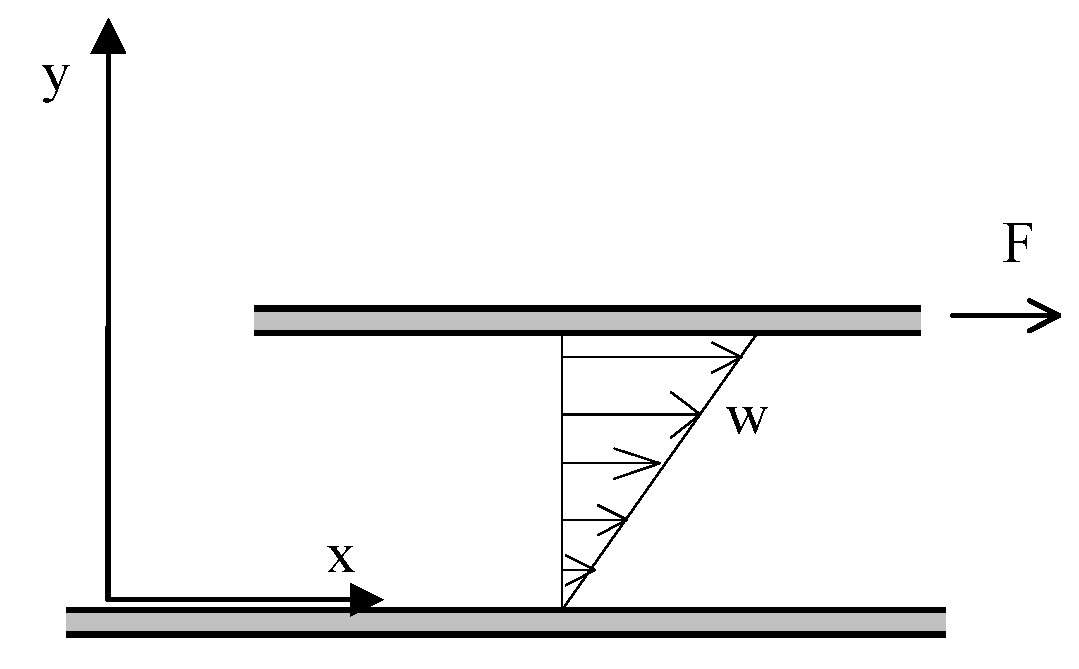
\includegraphics[width=0.6\textwidth]{fig/fluidodinamica/meato.eps}
    \caption{Azioni esercitate da un fluido tra due superfici in moto relativo \parencite{guglielmini2004lezioni}.} 
    \label{fig:meato}
\end{figure}
Il moto relativo tra fluido e parete è nullo, nel meato si crea quindi un campo di velocità triangolare, dove i piani di fluido scorrono l'uno sull'altro. Questo genera una forza resistente sulla superficie della parete superiore in moto. Indicando con \(A\) l'area della superficie di contatto tra  la lastra e il fluido, la forza resistente \(F\)  è espressa in modulo dalla legge di Newton:
\[F= \mu \; A \; \frac{dw}{dy} \implies \tau_{yx} = \frac{F}{A} = \mu \; \frac{dw}{dy} \addtag \label{eq:newton} \]
in cui \(\mu\) è una proprietà del fluido detta viscosità dinamica e \(\tau_{yx}\) rappresenta lo sforzo di taglio viscoso ovvero la forza che agisce per unità di area su  una superficie interna al fluido in direzione parallela a tale superficie, e \(\frac{dw}{dy}\) è la derivata della velocità del fluido rispetto alla componente verticale del moto. Lo sforzo di taglio è proporzionale alla viscosità e al gradiente di velocità. Il rapporto è direttamente proporzionale se i fluidi sono classificabili come newtoniani, cioè se la viscosità è indipendente dallo sforzo viscoso per determinate condizioni di temperatura e pressione. Per i fluidi non newtoniani vale la seguente formula:
\[\frac{dw}{dy}=\frac{\tau}{\mu(\tau)}\addtag\label{eq:newtoniani}\]
A seconda dell'andamento della funzione \(\mu(\tau)\) i fluidi possono essere classificati come "pseudo plastici" o "dilatanti" (\figref{fig:newtoniani}).
\begin{figure}[htbp] %Immagine reologia di un fluido
    \centering
    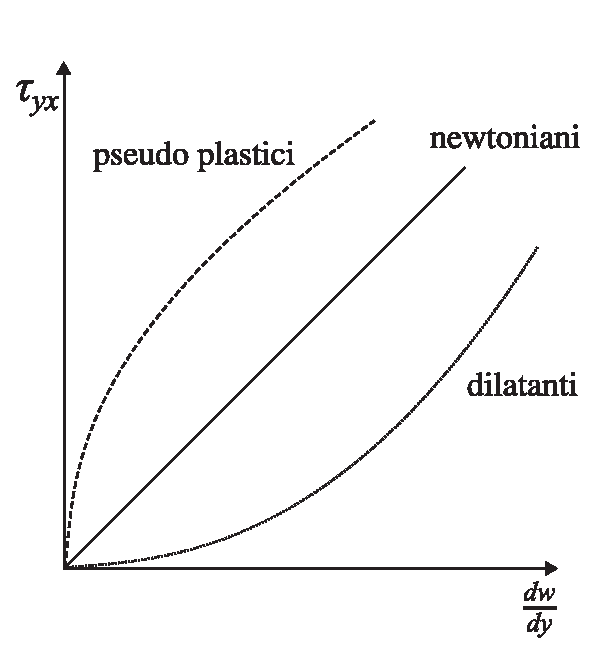
\includegraphics[width=0.5\textwidth]{fig/fluidodinamica/newtoniani.eps}
    \caption{Reologia di un fluido nel caso di fluidi newtoniani e non newtoniani \parencite{guglielmini2004lezioni}.} 
    \label{fig:newtoniani}
\end{figure}
\section[Moto e equazioni fondamentali]{Schematizzazione del moto e equazioni fondamentali di conservazione}
\sectionmark{Moto e equazioni fondamentali}
La rappresentazione analitica del moto di un fluido è assai complessa e richiede l'impiego di modelli al fine di semplificare la descrizione qualitativa e quantitativa di tale moto. Vengono indicate le tre figure fondamentali per la descrizione del moto di un fluido:
\begin{itemize}
\item \textbf{traiettoria di una particella}: il luogo dei punti occupati in tempi successivi dalla stessa particella fluida;
\item \textbf{linea di corrente} o \textbf{linea di flusso}: è una linea che ha per tangente il vettore velocità in ogni punto;
\item \textbf{linea di fumo}: è il luogo dei punti occupati, ad un dato istante, dalle particelle che sono passate per uno stesso punto.
\end{itemize}
Nel caso di moto permanente questi  tre luoghi geometrici coincidono. Si definisce vena fluida o filetto di corrente l'insieme delle traiettorie le cui sezioni trasversali hanno velocità (perpendicolare alla sezione stessa), pressione, temperatura e volume specifico costanti.\\
Il modello di riferimento è quello di moto uni- o monodimensionale e si assumono condizioni di regime permanente di massa e termodinamico. In termini fisici il modello deve rispettare i principi di:
\begin{itemize}
\item \textbf{conservazione della massa};
\item \textbf{conservazione della quantità di moto};
\item \textbf{bilancio di energia}.
\end{itemize}

\paragraph{Conservazione della massa}
Dato un sistema di coordinate cartesiane (x, y, z), si consideri un volume di controllo (VC) con gli spigoli \(dx\), \(dy\), \(dz\), attraversato da un fluido con velocità \(w\) e densità \(\rho\) (\figref{fig:vc}). Siano \(w_x\), \(w_y\) e \(w_z\) le componenti del vettore velocità lungo gli assi principali. Si definisce \(j\) velocità di massa o flusso di massa e si calcola la portata massica in entrata e in uscita sul VC lungo le tre direzioni principali. Se si sommano queste portate, si esprime la variazione di massa infinitesima \(dm\) nel tempo infinitesimo \(dt\) relativa al VC:
\[dm= - \left[\dfrac{\partial(\rho \; w_x)}{\partial x} + \dfrac{\partial(\rho \; w_y)}{\partial y} + \dfrac{\partial(\rho \; w_z)}{\partial z} \right]dx \; dy \; dz \; dt \label{eq:conservazione} \addtag \]
La massa di VC può essere espressa anche come il prodotto della densità del fluido per il volume :
\[m= \rho \; dx \; dy \; \label{eq:massa}\ \addtag \]
e la variazione nel tempo è:
\[dm = \dfrac{\partial}{\partial t}\rho \; dx \; dy \; dz \label{eq:varmassa} \addtag \]
Per il principio di conservazione della massa, la \eqref{eq:conservazione} e la \eqref{eq:varmassa} devono equivalersi:
\[\dfrac{\partial(\rho \; w_x)}{\partial x} + \dfrac{\partial(\rho \; w_y)}{\partial y} + \dfrac{\partial(\rho \; w_z)}{\partial z}= - \dfrac{\partial \rho}{\partial t} \addtag \label{eq:continuita} \]
La \eqref{eq:continuita} rappresenta l'equazione di continuità di un fluido in coordinate cartesiane e può essere anche essere scritta come:
\[ \vec{\nabla} (\rho \vec{w}) = -\dfrac{\partial \rho}{\partial t} \addtag \label{eq:continuitadiff} \]

\begin{figure}[htbp] 
    \centering
    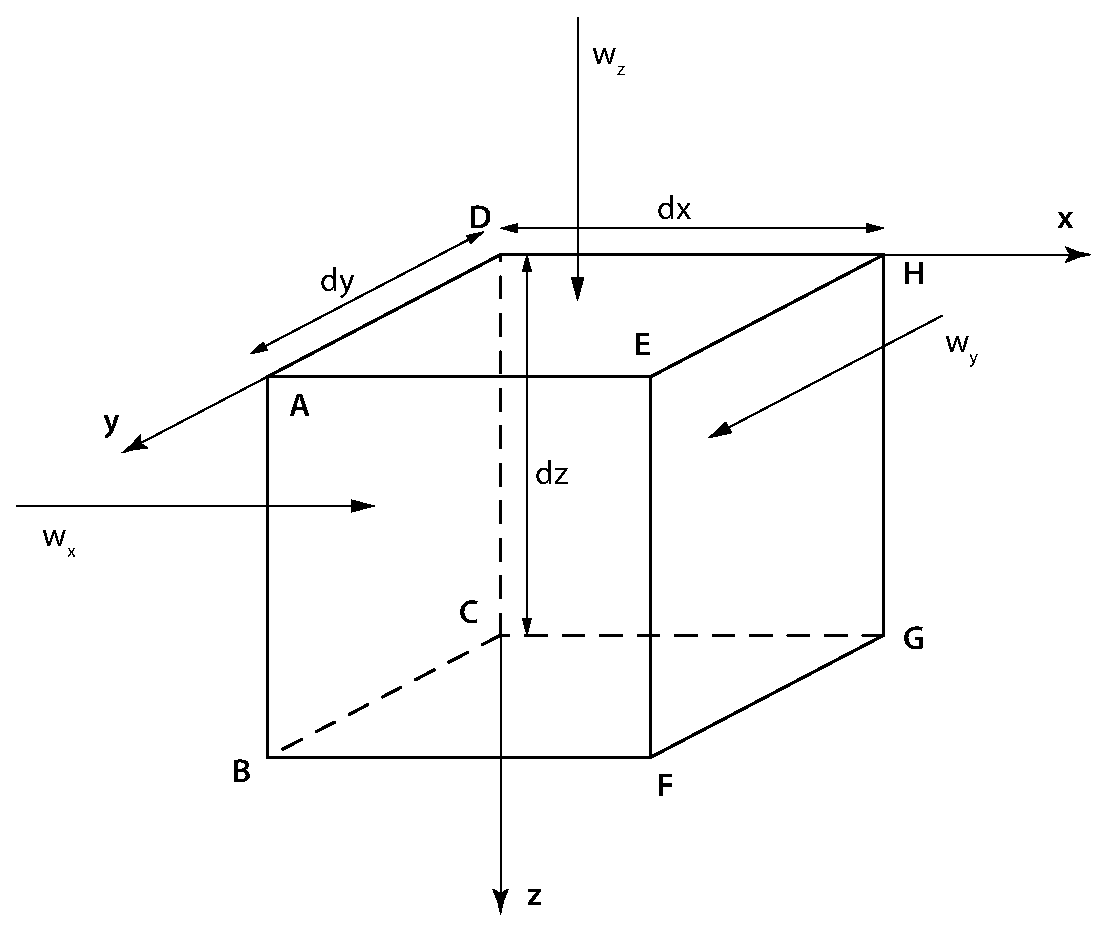
\includegraphics[width=.5\textwidth]{fig/fluidodinamica/cv.eps}
    \caption{Schematizzazione del parallelepipedo fondamentale o volume di controllo VC \parencite{chierici1989principi}.} 
    \label{fig:vc}
\end{figure}

\paragraph{Bilancio della quantità di moto}
La conservazione della quantità di moto è espressa dal secondo principio della dinamica. Dato un volume di controllo VC (definito precedentemente) la somma della variazione  della quantità di moto nel tempo \(dt\) del fluido di volume \(V\)e del flusso netto di quantità di moto attraverso la superficie \(S\) è uguale alla risultante delle forze esterne agenti sul fluido contenuto nel volume stesso.
In forma integrale:
\[\frac{d}{dt} \int_V \rho \vec w \, dV + \oint_A \left( \rho \vec w \right) \vec w \cdot \hat n \, dA = \int_V \vec F_V \, dV + \oint_A \underline{\underline T }\,dA \addtag \label{eq:intconsqm} \]
dove \(\underline{\underline T }\) rappresenta il tensore delle tensioni, \(\hat n\) il relativo versore e \(\vec F_V\) le forze di volume. In forma differenziale la \eqref{eq:intconsqm} diventa:
\[\rho \frac{D \vec w}{Dt} = \rho \vec F_V + \nabla \cdot \underline{\underline T } \addtag \]
che esprime il bilancio della quantità di moto per unità di volume.

\paragraph{Bilancio di energia e equazione di Bernoulli}
Tra le sezioni estreme di una generica vena fluida si applica l'equazione di bilancio dei sistemi aperti a regime permanente. Si considera come VC il volume racchiuso tra le due sezioni sopra citate. L'equazione di bilancio per unità di massa di un sistema aperto si può scrivere in forma differenziale come:
\[dQ-dL_e=dH+\frac{dw^2}{2}+gdz\addtag\]
dove $dQ$ e $dL_e$ rappresentano rispettivamente il calore scambiato con l'ambiente esterno e il lavoro esterno netto attraverso la superficie di confine, $dH$ rappresenta l'entalpia, $z$ la quota potenziale e \(g\) la costante di gravitazione universale (\(g \simeq 9,81\) m/s\ap{2}). Poiché $dh=TdS_s+vdp$:
\[dL_e+TdS_s+v \; dp+\frac{dw^2}{2}+g \; dz\label{eq:intermediobernoulli}\addtag\]
dove $dS_s$ è la produzione entropica elementare e $v$ il volume specifico. Un qualunque lavoro specifico, può essere espresso come prodotto di un volume specifico per un'opportuna pressione differenziale $dp'$, per omogeneità dimensionale. Questa variazione di pressione differisce dalla variazione che il fluido subisce in moto. Sapendo che una qualsiasi pressione $p$ può essere espressa in termini di peso specifico $\gamma$ e altezza idrica $h$:
\[dL_e=v\;dp_e=v\;\gamma\;dh_e=g\;dh_e\addtag\label{eq:lavoroesterno}\]
Allo stesso modo per il lavoro di attrito:
\[dL_a=v\;dp_a=v\;\gamma\;dh_a=g\;dh_a\addtag\label{eq:lavoroattrito}\]
Se sostituiamo la \eqref{eq:lavoroesterno} e la \eqref{eq:lavoroattrito} nella \eqref{eq:intermediobernoulli} otteniamo:
\[dh_e+dh_a+\frac{dp}{\gamma}+\frac{dw^2}{2g}+dz=0\label{eq:bernoulligeneralizzata}\addtag\]
La \eqref{eq:bernoulligeneralizzata} è detta equazione di Bernoulli generalizzata in forma differenziale e ha valenza energetica specifica (per unità di peso). I termini nella formula sono così nominati:
\begin{itemize}
    \item \(\mathbf{dh_e}\) \textbf{carico motore}, termine effettivo di scambio con l'esterno;
    \item \(\mathbf{dh_a}\) \textbf{carico d'attrito}, termine di dissipazione;
    \item \(\mathbf{\dfrac{dp}{\gamma}}\) \textbf{carico piezometrico}, l'effettiva variazione di pressione del fluido dovuta al moto;
    \item \(\mathbf{\dfrac{dw^2}{2g}}\) \textbf{carico cinetico};
    \item \(\mathbf{dz}\) \textbf{carico gravitazionale}, variazione di quota geodetica. 
\end{itemize}
Se la \eqref{eq:bernoulligeneralizzata} viene integrata tra la sezione 1 e la sezione 2 si ottiene:
\[(h_e)_{1,2}+(h_a)_{1,2}+\int^2_1{\frac{dp}{\gamma}}+\frac{w^2_2-w^2_1}{2g}+z_2-z_1=0\label{eq:bernoulliintegrata}\addtag\]
L'equazione caratterizzante il moto è così ridotta in termini di carichi differenziali, cioè in termini dimensionali si hanno delle lunghezze.\\
In caso di un condotto a pareti rigide, di sezione costante, orizzontale e attraversato da un fluido a regime permanente, cioè a carico motore e potenziale nullo, la \eqref{eq:bernoulliintegrata} diventa:
\[(h_a)_{1,2}+\int^2_1{\frac{dp}{\gamma}}+\frac{w^2_2-w^2_1}{2g}=0\label{eq:attritointermedio}\addtag\]
Se si ammettono trascurabili le variazioni di peso specifico rispetto alle variazioni di pressione, cioè si assume che il peso specifico sia costante, e la variazione di velocità nulla:
\[(h_a)_{1,2}=\frac{p_1-p_2}{\gamma}\label{eq:caricoattrito}\addtag\]
La \eqref{eq:caricoattrito} esprime il carico d'attrito o in termini operativi la perdita di carico. 
%%%%%%%%%%%%%%%%%%%%%%%%%%%%%%%%%%%%%%%%%%%%%%%%%%%%%%%%%%%%%%
\section{Calcolo delle cadute di pressione per attrito}
\subsection{Numero di Reynolds}
Si consideri un condotto rettilineo di diametro \(D\) a pareti perfettamente lisce in cui scorre un fluido a velocità \(w\), di densità \(\rho\) e viscosità \(\mu\). Il regime è definito laminare se le traiettorie del flusso sono rettilinee e il profilo di velocità è parabolico (\figref{fig:laminare}). Il regime di flusso è invece turbolento quando le particelle non seguono traiettorie ordinate e il moto che ne risulta avviene in maniera caotica (\figref{fig:turbolento}).

\begin{figure}[htbp]
\centering
    \subfloat[][Moto laminare]
    {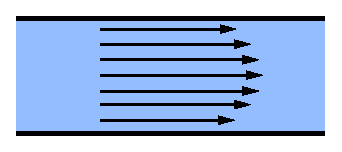
\includegraphics[width=.4\textwidth]{fig/fluidodinamica/laminareturbolento/laminare.eps} \label{fig:laminare}} \qquad \qquad
    \subfloat[][Moto turbolento]
    {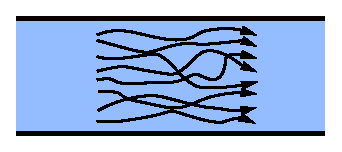
\includegraphics[width=.4\textwidth]{fig/fluidodinamica/laminareturbolento/turbolento.eps} \label{fig:turbolento}} \\
\caption{Regime di flusso monofase in condotta.}
\label{fig:laminareturbolento}
\end{figure}

Reynolds fu il primo a definire che il tipo di moto dovesse dipendere non solo dalla velocità ma anche dalla densità e viscosità del fluido, oltre che alla geometria della condotta. Il numero di Reynolds è così definito:
\[Re=\frac{\rho \; w \; D}{\mu}\addtag\label{eq:reynolds}\]
Il numero di Reynolds definisce il tipo di moto che si instaura in condotta:
\begin{itemize}
    \item per \(Re<2000\qquad\)il moto in un condotto è laminare;
    \item per \(2000<Re<10000\qquad\)si ha una regione di transizione;
    \item per \(Re>10000\qquad\)il moto in un condotto è completamente turbolento.
\end{itemize}
%%%%%%%%%%%%%%%%%%%%%%%%%%%%%%%%%%%%%%%%%%%%%%%%%%%%%%%%%%%%%%
\subsection{Fattore di attrito di Moody}
Sia in condizioni di moto laminare che in condizioni di moto turbolento, la caduta di pressione totale dipende dal tipo di fluido, dal regime di moto e dalle caratteristiche della condotta. In breve, il carico di attrito dipende da parametri:
\begin{itemize}
    \item \textbf{fisici} - \(\mu\) e \(\rho\) - relativi ai fluidi in movimento;
    \item \textbf{cinematici} - \(w\) - caratterizzanti il trasporto di massa fluida;
    \item \textbf{geometrici} - \(D\) e \(\epsilon\) - legati alla tubazione e alla scabrezza assoluta \(\epsilon\) della parete interna della condotta.
\end{itemize}
Perciò si può affermare che:
\[\frac{\Delta p}{l}=f(\rho, \; \mu, \; w, \; D, \; \epsilon) \addtag \label{eq:funzcaduta} \]
dove \(l\) è la lunghezza della condotta. L'equazione di Darcy-Weisbach può essere definita sia in funzione delle perdite di carico piezometriche \eqref{eq:darcyweisbachH} sia in funzione delle cadute di pressione \eqref{eq:darcyweisbachP}:
\[h_a = \lambda \; \frac{l}{D} \; \frac{w^2}{2 \; g} \addtag \label{eq:darcyweisbachH} \]
\[\Delta p_a = \lambda \; \frac{l}{D} \; \frac{\rho \; w^2}{2} \addtag \label{eq:darcyweisbachP} \]
dove \(\lambda\) è detto fattore d'attrito di Moody o indice di resistenza. La perdita di carico corrispondente, per un certo valore \(\lambda\), risulta proporzionale al carico cinetico e alla lunghezza del condotto. In regime di moto laminare il fattore di attrito è proporzionale al solo coefficiente di Reynolds:
\[\lambda=\frac{64}{Re} \addtag \]
In regime turbolento l'indice di resistenza è legata alla rugosità della parete. Il rapporto \(\frac{\epsilon}{D}\) è definito scabrezza relativa. La relazione funzionale equivalente è:
\[\lambda=f \; \left(Re, \; \frac{\epsilon}{D}\right) \addtag \]
Sulla base dei risultati sperimentali al variare dei parametri del modello di flusso in condotta in regime turbolento, è stato costituito il diagramma di Moody (\figref{fig:moody}). Gli andamenti all'interno di tale diagramma sono la rappresentazione grafica della correlazione di Colebrook:
\[ \frac{1}{\sqrt{\lambda}} = - 2 \ln \left( \frac { \epsilon/D} {3{,}71} + \frac {2{,}51} {Re \, \sqrt{\lambda}} \right) \addtag \label{eq:colebrook} \]

\begin{figure}[htbp] %Immagine diagramma di Moody
    \centering
    \includegraphics[width=.9\textwidth]{fig/fluidodinamica/moody.eps}
    \caption{Diagramma di Moody per il calcolo del fattore di attrito in condotta.} 
    \label{fig:moody}
\end{figure}

Il fattore di attrito può essere espresso anche tramite il numero di Fanning \(f\), adimensionale e definito come il rapporto tra gli sforzi di taglio e le forze di inerzia:
\[f=\dfrac{2\tau}{\rho w^2} \addtag \label{fanning} \]
Il fattore di attrito di Moody è quattro volte il numero di Fanning:
\[\lambda = 4f \addtag \label{eq:fanningmoody} \]
Blasius propone il calcolo del numero di Fanning a partire dal numero di Reynolds:
\[f=\dfrac{0,079}{Re^{0,25}} \addtag \label{eq:fanningreynolds} \]
La \eqref{eq:fanningreynolds} è applicabile in condizione di tubi a pareti interne lisce (scabrezza nulla, \(\epsilon=0\)) e regime di flusso non totalmente turbolento (\(Re<10^5\)).
%%%%%%%%%%%%%%%%%%%%%%%%%%%%%%%%%%%%%%%%%%%%%%%%%%%%%%%%%%%%%%%%%%%%%%
\subsection{Perdite di carico per un liquido}
Una relazione approssimativa per la valutazione delle perdite di carico di liquidi in condotta è quella di Hazen-Williams.  Questa relazione è valida solo per acqua in condizioni di regime turbolento a temperatura compresa tra i 4°C e 25°C.
\[\frac{h_a}{l} = \frac{10,65\ \dot{V}^{1,85}}{C^{1,85}\ d^{4,87}} \addtag \label{eq:HW}\]
dove \(dot V\) è la portata volumetrica, la costante moltiplicativa numerica 10,65 non è adimensionale (ha le dimensioni di \(s^{1,85}/m^{0,86}\)) e la costante adimensionale \(C\) è un valore tabellato.
\begin{table}[htbp]
    \small
    \centering
    \begin{tabular}{|l|r|}
        \hline
        \textbf{Tipologia tubo} & \(\mathbf{C}\)\\
        \hline
             Tubi estremamente lisci & 140\\
        Tubi nuovi, acciaio o ghisa & 130\\
        Tubi in legno o calcestruzzo & 120\\
        Tubi in acciaio rivettato, nuovi & 110\\
        Tubi vecchi in ghisa, mattoni & 100\\
        Tubi in acciaio rivettato, vecchi & 95\\
        Tubi in acciaio corroso & 80\\
        Tubi in acciaio fortemente corroso & 60\\
        \hline
    \end{tabular}
    \label{tab:coefficientiHZ}
    \caption{Coefficienti $C$ adimensionali per la formula di Hazen-Williams \parencite{dimarcopaolo2006appunti}.}
\end{table}
L'equazione fornisce direttamente il valore delle perdite di carico distribuite per unità di lunghezza della tubazione in funzione della portata volumetrica e del diametro idraulico. Se ora esplicitiamo la \eqref{eq:darcyweisbachH} in funzione del diametro interno \(D\), ponendo la portata volumetrica come \(\dot{V} =w \, A\):
\[h_a = \lambda \; \frac{l}{D} \; \frac{w^2}{2 \; g} \quad \implies \quad \frac{h_a}{l}=\frac{8 \, f}{\pi^2 \, 2g} \, \frac{{\dot{V}}^2}{D^5} \addtag \label{eq:darcyweisbachespl} \]
In entrambe le formulazioni (la forma generale delle perdite di carico e l'approssimazione di Hazen-Williams) si rileva che, a parità di portata, le perdite di carico sono inversamente proporzionali al diametro della tubazione elevato ad un esponente prossimo a 5.

%%%%%%%%%%%%%%%%%%%%%%%%%%%%%%%%%%%%%%%%%%%%%%%%%%%%%%%%
\subsection{Perdite di carico per un gas}
In condotte lunghe, il flusso di un gas è prossimo alle condizioni isotermiche. Le cadute di pressione in tali linee sono spesso grandi paragonate alla pressione in ingresso e il problema non può essere trattato tramite il modello di flusso di Darcy. Una soluzione accurata è data dall'equazione:
\[\dot{m}^2=\left[\dfrac{A^2}{v_1\left(\dfrac{\lambda\,l}{D}+2\ln\dfrac{p_1}{p_2}\right)}\right]\left[\dfrac{{p_1}^2-{p_2}^2}{p_1}\right] \addtag \label{eq:cpgasgenerale1}\]
dove \(\dot{m}\) è la portata massica, \(p_1\) e \(p_2\) sono le pressioni all'inizio e alla fine della condotta.
Se esplicitiamo nella \eqref{eq:cpgasgenerale1} il volume specifico in ingresso \(v_1\) utilizzando l'equazione di stato di un gas reale:
\[{p_1}^2-{p_2}^2=Z R T \left(\dfrac{w}{A}\right)^2\left(\lambda \, \dfrac{l}{D}+2\ln\dfrac{p_1}{p_2}\right)  \addtag \label{eq:cpgasgenerale2}\]
dove \(Z\),  è il fattore di comprimibilità del gas, \(R\) è la costante universale dei gas perfetti e \(T\) la temperatura.
Si formulino le seguenti assunzioni:
\begin{itemize}
    \item flusso di gas a condizioni isotermiche;
    \item assenza di lavoro meccanico in ingresso e uscita;
    \item regime permanente;
    \item gas perfetto;
    \item velocità come rappresentazione della velocità media nella sezione trasversale;
    \item coefficiente d'attrito \(\lambda\) costante;
    \item condotta dritta e orizzontale
\end{itemize}
La \eqref{eq:cpgasgenerale1} e la \eqref{eq:cpgasgenerale2} possono essere scritte semplificate in:
\[\dot{m}^2=\left[ \dfrac{D \, A^2}{v_1 \, \lambda \, l}\right] \left[\dfrac{{p_1}^2-{p_2}^2}{p_1}\right] \addtag \label{eq:cpgassempl1} \]

\[{p_1}^2-{p_2}^2=Z_m R T \left(\dfrac{w}{A}\right)^2\left(\lambda \, \dfrac{l}{D}\right)  \addtag \label{eq:cpgassempl2}\]
Possono essere utilizzate tre diverse forme semplificate per il calcolo delle portate di gas in condotta, a seconda delle specifiche tecniche dell'infrastruttura.

\paragraph{Equazione di Weymouth}
L'equazione di Weymouth è raccomandata per condotte con diametro piccolo (generalmente sotto i 12") e lunghezza limitata (sotto i 30 km) all'interno delle batterie di produzione o per le linee di raccolta secondarie, pressione medio-alta (compresa tra 7 bar e 70 bar) in regime di moto turbolento (alto valore del numero di Reynolds).
\[\dot{V}_h=2,61\e{-8} \; {D_{mm}}^{2,667} \; \left[ \left(\dfrac{p_1^2 - p_2^2}{\rho_r \, l_{km}}\right) \dfrac{288}{T_1} \right]^{0.5} \addtag \label{eq:weymouth} \]
dove \(\dot{V}_h\) è la portata espressa in Smc\footnote{\textit{Standard metri cubi}, quantità di gas contenuta in un 1 m\ap{3} a condizioni standard di pressione (\(p=101325\) Pa, pressione ambientale) e di temperatura  (\(T=288,15\) K, 15°C)}/h, \(\rho_r\) è la densità relativa, \(D_{mm}\) è il diametro interno della condotta espresso in mm, \(l_{km}\) è la lunghezza della condotta espressa in km.

\paragraph{Equazione di Panhandle}
L'equazione di Panhandle è indicata per condotte di grande diametro (pari o sopra i 12"), condotte lunghe (più di 70 km) e per valori del numero di Reynolds moderati. 
\[\dot{V}_h=2,044\e{-8} \; \phi \;{D_{mm}}^{2,6182} \; \left( \dfrac{p_1^2 - p_2^2}{l_{km}} \right)^{0,5394} \addtag \label{eq:pandhandle} \]
dove \(\phi\) rappresenta il fattore di efficienza del flusso (\(\phi \leq 1\), ha valore unitario in caso di nuove condotte)

\paragraph{Equazione di Spitzglass}
Esistono due versioni di questa equazione: ad alta o bassa pressione. L'equazione di Spitzglass relativa a condotte a bassa pressione è:
\[\dot{V}_h = 9,50 \; \left[ \dfrac{(p_1-p_2) \; {D_{mm}}^5 }{l_{mm} \; \rho_r \; (1+0,09144/D_{mm} + 1,1811 \; D_{mm}) } \right]^2 \addtag \label{eq:spitzglass}\]


\subsection{Perdite di carico concentrate}
Il fluido, lungo il suo percorso in condotta, può incontrare brusche variazioni di sezione, direzione o ostruzioni come filtri o rubinetti. Il calcolo delle resistenze puntuali è difficilmente calcolabile in modo analitico e ci si basa maggiormente su dati puramente sperimentali. Tutte le resistenze relative a diversi elementi tipici della condotta sono espresse in funzione del carico cinetico:
\[\Delta p' = \gamma \; \frac{w^2}{2g} \; f' \addtag \label{eq:concentrate}\]
dove \(f'\) assume valori diversi a seconda del tipo di singolarità. La somma di perdite di carico concentrate e distribuite fornisce la caduta di pressione totale per una generica condotta percorsa da un fluido.

%%%%%%%%%%%%%%%%%%%%%%%%%%%%%%%%%%%%%%%%%%%%%%%%%%%%%%%%%%
\section{Moto multifase}
In termodinamica classica si definisce fase come uno stato macroscopico della materia omogeneo per struttura fisica e composizione chimica. I flussi bifase sono caratterizzati dalla presenza di due fasi e rappresentano il caso più semplice di flusso multifase o multicomponente. Nei flussi bifase, l'iterazione tra le due fasi porta alla formazione di particolari regimi di flusso. Il verificarsi di un determinato regime dipende dalla portata, dalle caratteristiche fisiche e dalle condizioni termodinamiche delle due fasi e dalle caratteristiche fisiche dell'impianto.

\subsection{Regime di flusso in condotta}
L'inclinazione della condotta incide fortemente sulla formazione dei diversi regimi di flusso: in caso di tubazioni verticali, la forza gravitazionale agisce nella stessa direzione della forza inerziale, quindi lungo l'asse della condotta. In condotte verticali si hanno quindi regimi pseudo-simmetrici rispetto l'asse della condotta, in tubazioni orizzontali la fase liquida e la fase gassosa tendono a disporsi rispettivamente sulla parte inferiore e superiore. 

\subsubsection{Condotte verticali} \label{sssec:verticali}
I regimi di flusso bifase per condotte verticali sono così classificati (\figref{fig:verticale}):
\begin{itemize}
    \item flusso a bolle;
    \item flusso a \textit{slug};
    \item flusso a churn o agitato;
    \item flusso anulare misto.
\end{itemize}

\begin{figure}[htbp]
\centering
    \subfloat[][Flusso a bolle]
    {\makebox[0.2\textwidth]{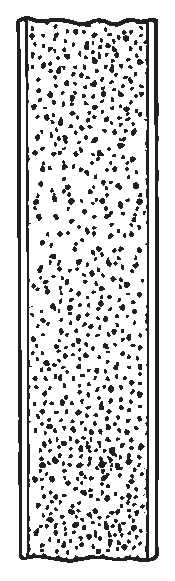
\includegraphics[width=.1\textwidth]{fig/fluidodinamica/vertical/ver-bubble.eps}} \label{fig:ver-bubble}} \quad
    \subfloat[][Flusso a \textit{slug}]
    {\makebox[0.2\textwidth]{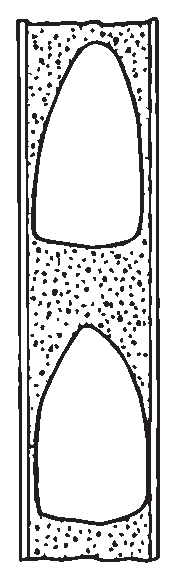
\includegraphics[width=.1\textwidth]{fig/fluidodinamica/vertical/ver-slug.eps}} \label{fig:ver-slug}}  \quad
    \subfloat[][Flusso a churn o agitato]
    {\makebox[0.2\textwidth]{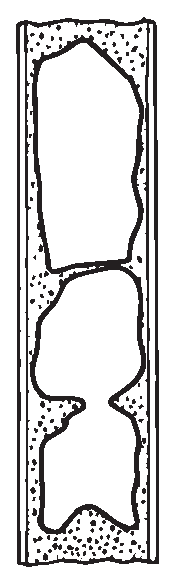
\includegraphics[width=.1\textwidth]{fig/fluidodinamica/vertical/ver-annular.eps}} \label{fig:ver-churn}} \quad
    \subfloat[][Flusso anulare misto]
    {\makebox[0.2\textwidth]{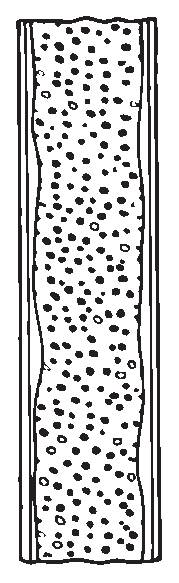
\includegraphics[width=.1\textwidth]{fig/fluidodinamica/vertical/ver-mist.eps}} \label{fig:ver-annular} }
\caption{Regimi di flusso bifase in condotte verticali \parencite{lake2006petroleum}.}
\label{fig:verticale}
\end{figure}

Per comprendere nel dettaglio i vari regimi che si possono instaurare in condotta si fa riferimento alla mappa dei regimi di flusso bifase avvallata da \textcite{griffith1984multiphase} per condotte verticali (\figref{fig:ver-griffith}).

\begin{figure}[htbp]
    \centering
    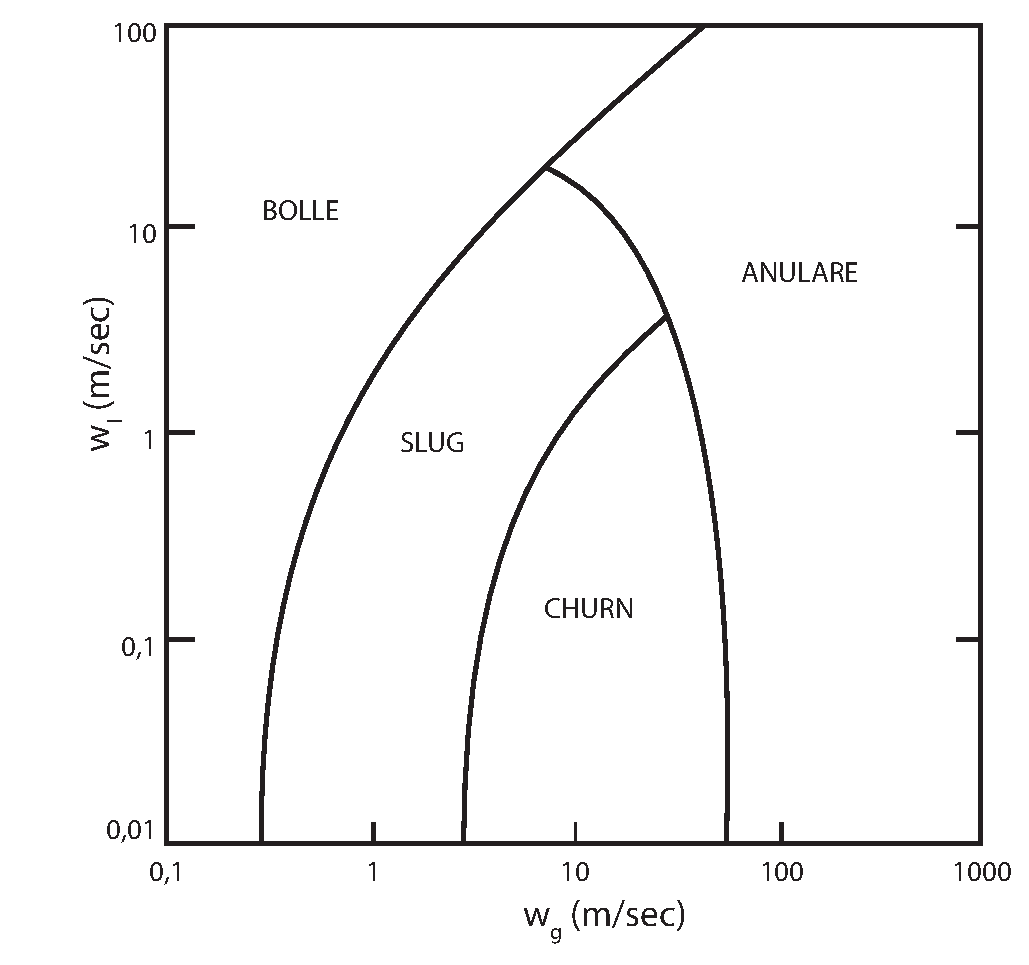
\includegraphics[width=.6\textwidth]{fig/fluidodinamica/ver-griffith.eps}
    \caption{Mappa per regimi di flusso bifase per condotte verticali \parencite{griffith1984multiphase}.}
    \label{fig:ver-griffith}
\end{figure}

Per basse velocità superficiali della fase gassosa, avviene in condotta il solo regime a bolle (\figref{fig:ver-bubble}). In questo regime la fase liquida si muove a velocità uniforme mentre le bolle di gas sono più veloci o più lente a seconda del loro diametro. Se si incrementa la velocità della fase gassosa, questa tenderà a viaggiare di pari passo alla fase liquida, creando così il regime a \textit{slug} (\figref{fig:ver-slug}) e il regime a churn o anche detto agitato (\figref{fig:ver-churn}), dove ormai l'effetto della fase gassosa è predominante rispetto alla fase liquida. Nel regime anulare misto (\figref{fig:ver-annular}) la fase gassosa è continua e la fase liquida è dispersa nel gas oppure disposta sulle pareti interne.

\subsubsection{Condotte orizzontali}
I regimi di flusso in condizioni di condotta orizzontale possono essere così classificati (\figref{fig:orizzontale}):
\begin{itemize} 
    \item flusso stratificato;
    \item flusso a onde;
    \item flusso a \textit{plug} o a bolle allungate;
    \item flusso a \textit{slug};
    \item flusso anulare;
    \item flusso a bolle disperse.
\end{itemize} 

\begin{figure}[htbp]
\centering
    \subfloat[][Flusso stratificato]
    {
\includegraphics[width=.4\textwidth]{fig/fluidodinamica/horizontal/hor-stratified.eps} \label{fig:hor-stratified}} \qquad \qquad
    \subfloat[][Flusso a onde]
    {
\includegraphics[width=.4\textwidth]{fig/fluidodinamica/horizontal/hor-wavy.eps} \label{fig:hor-wavy}} \\
    \subfloat[][Flusso a \textit{plug}]
    {
\includegraphics[width=.4\textwidth]{fig/fluidodinamica/horizontal/hor-plug.eps} \label{fig:hor-plug}} \qquad \qquad
    \subfloat[][Flusso a \textit{slug}]
    {
\includegraphics[width=.4\textwidth]{fig/fluidodinamica/horizontal/hor-slug.eps} \label{fig:hor-slug}}\\
    \subfloat[][Flusso anulare]
    {
\includegraphics[width=.4\textwidth]{fig/fluidodinamica/horizontal/hor-annular.eps} \label{fig:hor-annular}} \qquad \qquad
    \subfloat[][Flusso a bolle disperse]
    {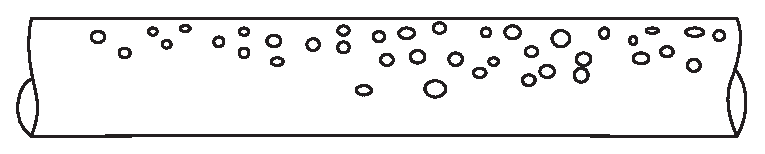
\includegraphics[width=.4\textwidth]{fig/fluidodinamica/horizontal/hor-bubble.eps} \label{fig:hor-bubble}}
\caption{Regimi di flusso bifase in condotte orizzontali \parencite{lake2006petroleum}.}
\label{fig:orizzontale}
\end{figure}
Per la determinazione dei diversi regimi di flusso bifase aria-acqua si fa riferimento alle mappe per condotte orizzontali proposte da \textcite{griffith1984multiphase}, \textcite{baker1954simultaneous} e \textcite{taitel1976model}.

\paragraph{\textcite{griffith1984multiphase}}
Il regime di flusso è definito tramite la velocità superficiale \(w_i\), legata alla portata volumetrica della fase i-esima attraverso una generica sezione \(A\) della condotta. Si ha quindi:
\[\dot{V}_g = \frac{\dot{V}_g}{A} \addtag\]
\[w_l = \frac{\dot{V}_l}{A} \addtag\]
dove i pedici \(g\) e \(l\) fanno riferimento alla fase gassosa o liquida. Le linee continue interne rappresentano la transizione tra i diversi regimi.\\
Per basse velocità superficiali della fase liquida si verificano flussi stratificati a interfaccia liscia (\figref{fig:hor-stratified}), a onda (\figref{fig:hor-wavy}) e anulare misto (\figref{fig:hor-annular}) a seconda della velocità superficiale del liquido. Questi tre regimi fanno parte della categoria dei flussi separati: le due fasi appaiono come due flussi continui senza apparente iterazione. Il flusso stratificato e quello a onde sono caratterizzati dallo scorrimento della fase liquida nella parte inferiore della condotta, in quello anulare la fase liquida si dispone lungo le pareti interne della condotta. All'aumentare della velocità superficiale della fase liquida, si osserva un maggiore miscelamento delle due fasi e si verificano flussi a \textit{slug} o a bolle allungate (\figref{fig:hor-slug}) o flussi a \textit{plug} (\figref{fig:hor-plug}). La differenza tra questi due regimi è sottile: nel flusso a \textit{slug} sono disperse numerose bollicine di gas nella fase liquida, al contrario del flusso a \textit{plug}. Ad alte velocità superficiali della fase liquida si verifica il flusso a bolle (\figref{fig:hor-bubble}), caratterizzato dalla presenza di bolle di gas disperse nella fase liquida.
\begin{figure}[htbp]
    \centering
    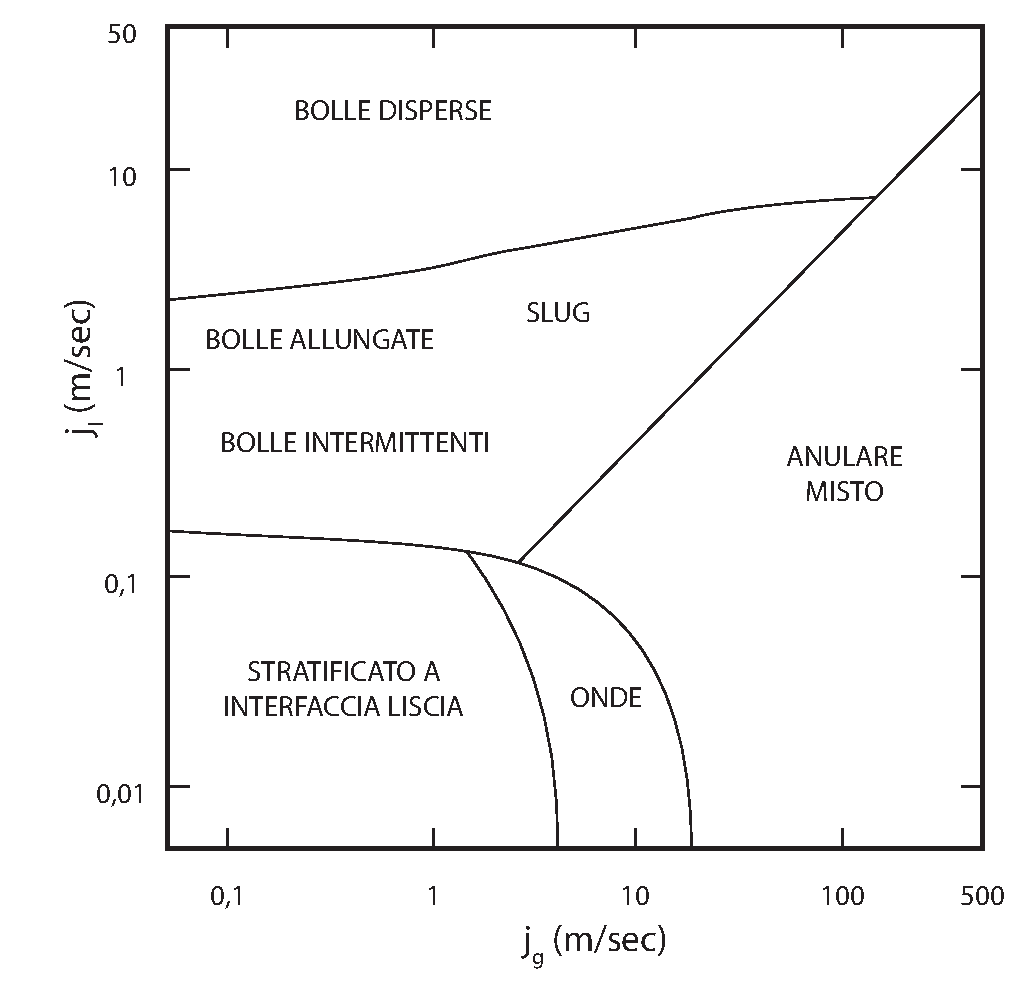
\includegraphics[width=.6\textwidth]{fig/fluidodinamica/hor-griffith.eps}
    \caption{Mappa di \textcite{griffith1984multiphase} per regimi di flusso bifase per condotte orizzontali.}
    \label{fig:hor-griffith}
\end{figure}

\paragraph{\textcite{baker1954simultaneous}}
La mappa di \textcite{baker1954simultaneous} per condotte orizzontali con flusso bifase (\figref{fig:baker}) è stata proposta originariamente sia nel Sistema Internazionale che nel sistema consuetudinario statunitense. Per l'utilizzo della mappa devono essere determinati i parametri adimensionali \(\Lambda\) e \(\Psi\) e la velocità di massa o flusso di massa \(j_i\), la massa della fase i-esima che attraversa una generica sezione trasversale \(A\) della condotta:
\[j_g = \frac{\dot{m_g}}{A}=\frac{\rho_g w_g A}{A}=\rho_g w_g \addtag\]
\[j_l = \frac{\dot{m_L}}{A}=\frac{\rho_l w_l A}{A}=\rho_l w_l \addtag\]
dove \(j_G\) e \(j_l\) sono (in modulo) la velocità di massa del gas e del liquido. I parametri adimensionali \(\Lambda\) e \(\Psi\) sono definiti da:
\[\Lambda= \left(\dfrac{\rho_g}{\rho_{aria}} \dfrac{\rho_l}{\rho_{acqua}}\right)^{1/2} \addtag \label{eq:lambdabaker} \]
\[\Psi=\left( \frac{\sigma_{acqua}}{\sigma} \right) \left[ \left( \frac{\mu_L}{\mu_{acqua}} \right) \left( \frac{\rho_{acqua}}{\rho_l} \right)^2 \right]^{1/3} \addtag \]
dove \(\rho_g\), \(\rho_l\), \(\mu_L\) e \(\sigma\) sono proprietà proprie del fluido. I termini noti, quindi le proprietà di riferimento sono:
\begin{itemize}
    \item \(\rho_{acqua}=1000\) kg/m\ap{3};
    \item \(\rho_{aria}=1,23\) kg/m\ap{3};
    \item \(\mu_{acqua}=0,001\) N sec/m\ap{2};
    \item \(\sigma_{acqua}=0,072\) N/m.
\end{itemize}
I valori sugli assi x e y sono così identificati. L'intersezione sulla mappa fornisce il regime bifase che si instaura nella condotta sulla base del modello.
\begin{figure}[htbp]
    \centering
    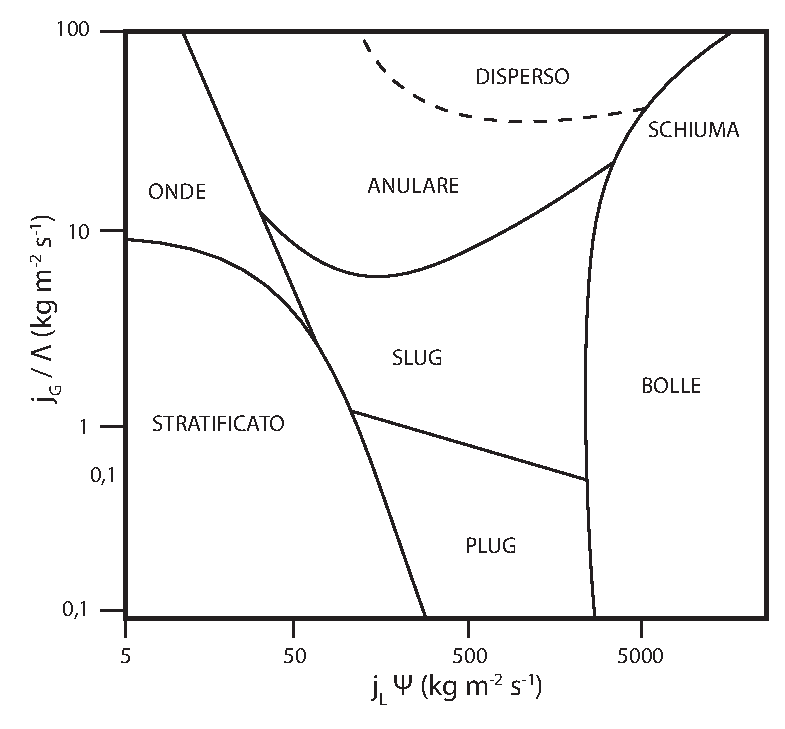
\includegraphics[width=.6\textwidth]{fig/fluidodinamica/baker.eps}
    \caption{Mappa di \textcite{baker1954simultaneous} per regimi di flusso bifase per condotte orizzontali.}
    \label{fig:baker}
\end{figure}

\paragraph{\textcite{taitel1976model}}
Nel lavoto di \textcite{taitel1976model} (\figref{fig:taitel}) si propone una mappa per condotte orizzontali che nasce dalla combinazione di analisi analitiche e selezione empirica di numerosi parametri di riferimento. La mappa usa il parametro di Martinelli \(\chi\), il numero di Froude del gas \(Fr_g\) e i parametri \(T\) e \(K\).

\begin{figure}[htbp]
    \centering
    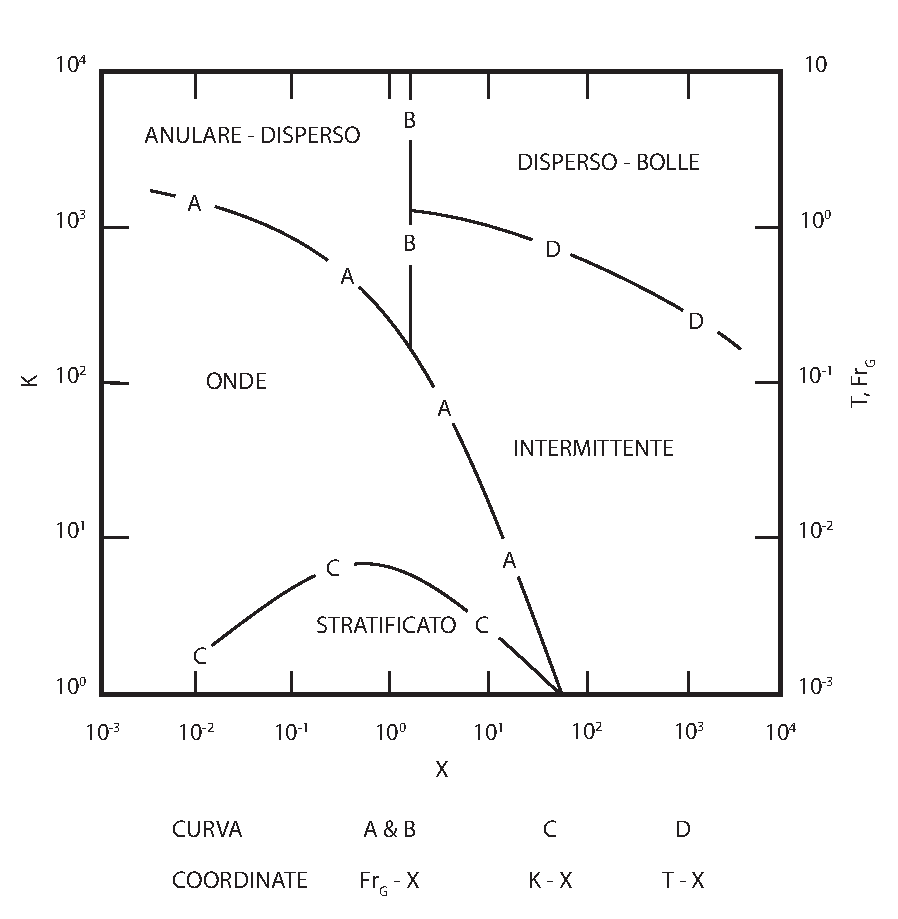
\includegraphics[width=.6\textwidth]{fig/fluidodinamica/taitel.eps}
    \caption{Mappa di \textcite{taitel1976model} per regimi di flusso bifase per condotte orizzontali. Gli assi di riferimento cambiano a seconda della curva considerata, come descritto nel pannello al di sotto del grafico.}
    \label{fig:taitel}
\end{figure}

Il parametro di Martinelli è dato dalla radice quadrata del rapporto tra i gradienti di pressione del liquido e del gas:
\[\chi = \left[ \frac{(dp/dl)_L}{(dp/dl)_G} \right]^{1/2} \addtag \label{eq:martinelli} \]
Si ricorda che il gradiente di pressione per unità di lunghezza è dato dalla derivata dell'equazione di Darcy-Weisbach \eqref{eq:darcyweisbachP} in funzione della caduta di pressione lungo la direzione della condotta:
\[\Delta p_{a,k} = \lambda_k \; \frac{l}{D} \; \frac{\rho_k \; w_k^2}{2} \implies \left(\dfrac{dp}{dl}\right)_k =- \frac{\lambda_k}{D} \; \frac{\rho \; w^2}{2} = - \frac{\lambda_k \; j_k^2}{\rho_k \; D}  \addtag \label{eq:gradientepressione} \]
Il numero di Froude è un gruppo adimensionale e rappresenta la frazione liquida di un fluido.  Dal punto di vista analitico mette in relazione forza di inerzia con la forza peso. Per la fase gassosa vale:
\[Fr_g = \frac{j_g}{[\rho_g(\rho_l-\rho_g)D \; g]^{1/2}} \addtag \label{eq:froude}\]
Il parametro \(T\) è definito come:
\[ T = \left[ \dfrac{|(dp/dl)_L|}{g(\rho_l-\rho_g)} \right]^{1/2} \addtag \label{parametroT} \]
Il parametro \(K\) invece è funzione del numero di Froude del gas e del numero di Reynolds del liquido:
\[K=Fr_g \; Re_L^{1/2} \addtag \label{parametroK} \]
Caratteristica principale di questa mappa di regime è l'impiego di diverse coordinate, in funzione dei parametri trovati, a seconda della curva a cui si fa riferimento. Dapprima si calcolano quindi il parametro di Martinelli \(\chi\) e il numero di Froude del gas \(Fr_g\). Se le coordinate del punto trovato ricadono nella parte superiore della curva A, rappresentata rispetto al sistema di coordinate \(Fr_g-\chi\), il regime sarà quindi anulare. Nel caso in cui il punto si collochi al di sotto della curva viene calcolato il parametro \(K\). Facendo riferimento alla curva C e quindi al sistema di coordinate \(K-\chi\) il regime sarà a onde o stratificato con interfaccia liscia se il punto trovato è rispettivamente nella parte superiore o inferiore della curva C. Se il punto ricade nella parte superiore a destra del grafico, si fa riferimento alla curva D, quindi al sistema di coordinate \(T - \chi \). Il regime sarà a bolle disperse se il punto trovato si trova al di sopra della curva D, viceversa il regime sarà di natura intermittente o a \textit{slug}. \\
Tutti i modelli fin qui presentati sono stati sviluppati per flussi bifase in condizioni adiabatiche. Tuttavia questi modelli, tramite accorgimenti di natura analitica, possono rispondere anche a condizioni diabatiche, cioè ipotizzando la condotta come sistema aperto in cui avviene scambio di calore con l'esterno. Lo studio dei regimi di flusso può quindi essere esteso, per esempio, negli impianti di refrigerazione oppure negli scambiatori termici.

\subsection{Cadute di pressione per attrito di un flusso bifase}
Si può semplificare lo studio del moto di un fluido bifase se si assume che le fasi siano ben miscelate fra loro, quindi come un unico fluido monofase. Il modello omogeneo può essere applicato quando le fasi sono fortemente interdisperse tra loro, cioè quando entrambe hanno velocità superficiali sostenute. Le perdite di carico totali \(\Delta p_{tot}\) sono la somma delle perdite di carico statiche o gravitazionali \(\Delta p_s\), le perdite di carico della quantità di moto \(\Delta p_{mom}\) e le perdite di carico per attrito \(\Delta p_a\): 
\[\Delta p_{tot} = \Delta p_s +\Delta p_{mom} + \Delta p_a \addtag \label{eq:perditetot}\]
La perdita di carico statico per un fluido bifase omogeneo è:
\[\Delta p_s = \rho_h \; g \; z\ \addtag \]
dove \(z\) è la differenza di quota geodetica tra le sezioni di ingresso e uscita della condotta, o meglio l'altezza della condotta. Per densità omogenea \(\rho_h\) si intende:
\[\rho_h=\rho_l(1-\xi_h)+\rho_g \; \xi_h \addtag \label{eq:omogenea} \]
Si determina la frazione di vuoto \(\xi_h\) in funzione del titolo di vapore \(x\):
\[\xi_h = \left[ 1+ \left( \dfrac{w_g}{w_l} \dfrac{(1-x)}{x} \dfrac{\rho_g}{\rho_l} \right) \right]^{-1} \addtag \]
dove il rapporto \(w_g/w_l\) è detto rapporto di slittamento e ha valore unitario nel caso di flussi omogenei. Il gradiente di pressione della quantità di moto per unità di lunghezza del condotto è:
\[\left( \dfrac{dp}{dl} \right)_{mom}=\dfrac{d(j_{tot}/\rho_h)}{dz} \addtag \]
Il punto cruciale del calcolo delle cadute di pressione per un flusso bifase risiede nella stima del termine di attrito, in questo frangente rappresentato dal numero di Fanning \(f\). Se si esprime la \eqref{eq:darcyweisbachP} in funzione del numero di Fanning \(f_{tot}\) per un flusso bifase, in funzione del flusso di massa \(j_{tot}\):
\[\Delta p_a = \dfrac{2 \; f_{tot} \; j_{tot}^2}{\rho_{tot}} \; \dfrac{l}{D} \addtag \label{eq:darcyweisbachfanning2f} \]
Si può esprimere il numero di Fanning tramite la \eqref{eq:fanningreynolds}, il numero di Reynolds per mezzo della \eqref{eq:reynolds}. Come viscosità, parametro utile al calcolo del numero di Reynolds, può essere scelta quella della fase liquida oppure una media pesata in base al titolo di vapore \(x\):
\[\mu_{tot} =x \; \mu_G + (1+x) \; \mu_L \addtag \]
\\
\'E importante acquisire le basi della fluidodinamica multifase per capire come le iterazioni tra le diverse fasi e le perdite di carico definiscano il flusso che si instaura in condotta. L'ingegneria petrolifera ha affinato negli anni i modelli interpretativi, così da avvicinare le stime di produzione di un pozzo ai trend reali. In particolar modo, la corretta interpretazione del moto multifase per i pozzi a gas determina la tipologia e la configurazione di sistemi per l'aumento di portata o la diminuzione delle perdite di carico. Si intuisce quindi che l'aumento delle performance è legato alla veridicità del modello calcolato. Nel prossimo capitolo sono trattati i problemi di un pozzo a gas legati a condizioni di flusso multifase e le tecnologie oggi utilizzate per ovviare al calo di rendimento nel tempo.
%\section{Moto dei fluidi comprimibili in condotta a sezione variabile}
%\subsection{Velocità del suono}
%\subsection{Equazione di Hugoniot e numero di Mach}
%\subsection{Propagazione dei disturbi in flussi subsonici e supersonici}
%\subsection{Proprietà al ristagno}
%\subsection{Flusso attraverso un'onda d'urto normale}


\clearpage{\pagestyle{empty}\cleardoublepage}
\chapter{Applicazioni di schiumogeno per l'ottimizzazione della produzione degli idrocarburi}
\chaptermark{Applicazioni di schiumogeno}
Per \textit{Gas Well Deliquification} o \textit{Gas Well Dewatering} si intende l'insieme delle tecnologie e delle applciazioni utili alla rimozione di acqua o condensati in fase produttiva da un pozzo a gas. Nello specifico il concetto di GDW racchiude tutti gli strumenti utili nel combattere il fenomeno del \textit{liquid loading}, definito come l'impossibilità di un pozzo a gas di rimuovere liquidi prodotti in pozzo. Le tecnologie impiegate per lo spiazzamento dei liquidi a fondo pozzo sono numerose e sono in continua evoluzione per garantire migliori performance e affidabilità. Nell'ultimo decennio gli schiumogeni sembrano rappresentare una scelta concreta per controllare il carico idrostatico di fondo pozzo e presentano notevoli vantaggi rispetto alle tecnologie già esistenti \parencite{stanculescu2014gwd}. In questo capitolo sono descritte le cause e le conseguenze del \textit{liquid loading} e le principali tecnologie impiegate oggi per la riduzione e controllo del battente idrostatico. Particolare attenzione è dedicata all'impiego di tensioattivi liquidi o \textit{foamer}, descrivendo le proprietà fisico-chimiche, le procedure operative per il loro impiego e controllo tramite l'uso di antischiuma o  \textit{defoamer}.

\section{Liquid loading}
\subsection{Ciclo di vita di un pozzo a gas}
Nel paragrafo \ref{sssec:verticali} si è discusso dei diversi regimi di flusso bifase per condotte verticali. Un pozzo a gas può presentare tutti i regimi di flusso: in \figref{fig:wellhistory} è possibile comprendere graficamente l'evoluzione del pozzo durante il suo ciclo di vita.

\begin{figure}[htbp]
    \centering
    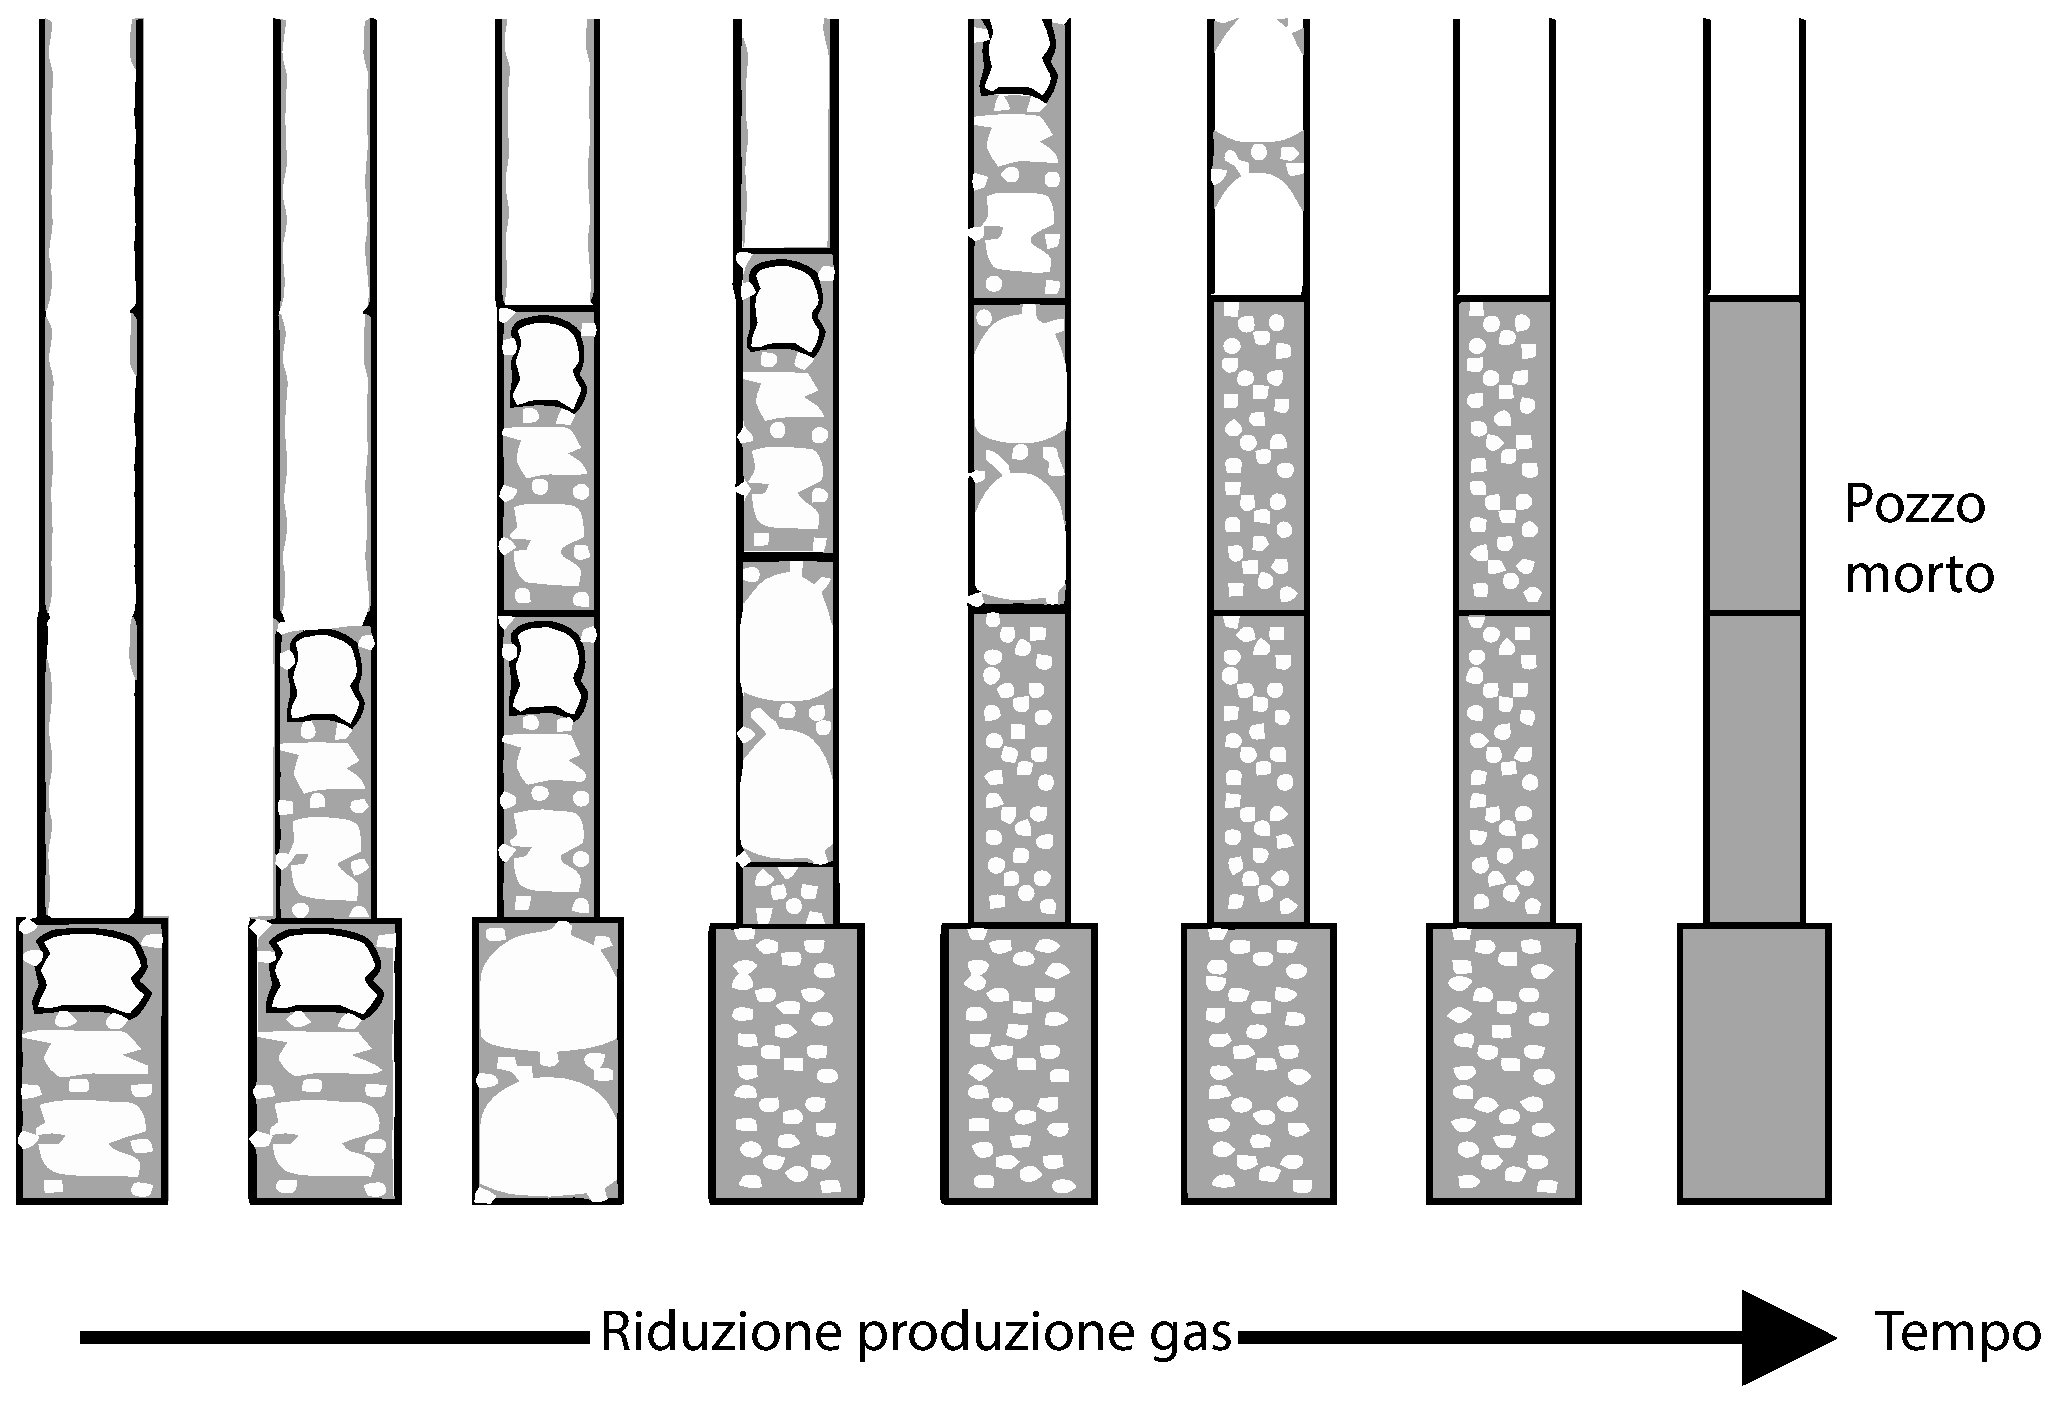
\includegraphics[width=.8\textwidth]{fig/foamer/wellhistory.eps}
    \caption{Schematizzazione del ciclo di vita di un pozzo a gas \parencite{lea2011gas}.}
    \label{fig:wellhistory}
\end{figure}

Generalmente in un pozzo sono presenti tutti i diversi regimi di flusso, con il passare del tempo varia la distribuzione dei diversi pattern lungo il tubino di produzione. Inizialmente il gas è fase dominante e il pozzo ha forza sufficiente per trascinare tutto il liquido presente sul fondo. Ad alte velocità superficiali del gas corrisponde un regime anulare misto: la fase liquida è interdispersa nella fase gassosa. Con il diminuire della velocità del gas nel tempo, la fase liquida comincia a precipitare e a depositarsi sul fondo, ostacolando la normale produzione di gas.

\subsection{Problemi legati al liquid loading}
Il liquid loading porta a un regime di flusso a slug e a una produzione di gas discontinua e inferiore. Se il gas ha energia sufficiente a rimuovere i liquidi presenti a fondo pozzo, la portata del gas risponde in modo corretto alla stima di produzione rispetto al tempo di vita del pozzo, definita tramite l'analisi della curva di declino (\textit{Decline Curve Analysis}, DCA), visibile in \figref{fig:declinecurve}.

\begin{figure}[htbp]
    \centering
    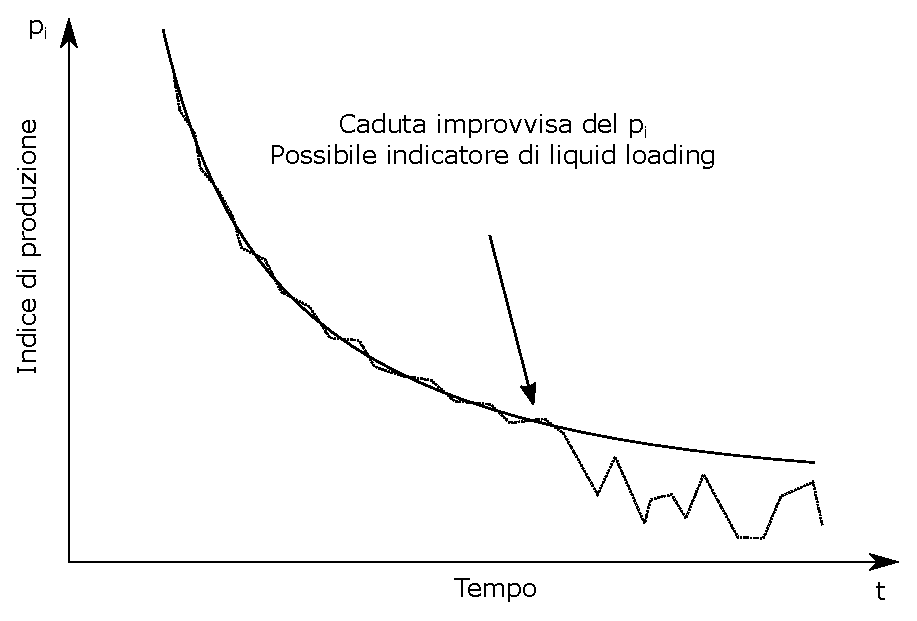
\includegraphics[width=.8\textwidth]{fig/foamer/declinecurve.eps}
    \caption{Analisi della curva di declino.}
    \label{fig:declinecurve}
\end{figure}

In caso di aumento del battente idrostatica, il pozzo produce gas in quantità minore rispetto alle stime effettuate. Raggiunto uno stato critico di produzione, il giacimento non ha più energia sufficiente per lo spiazzamento del pozzo e l'effetto combinato di precipitazione di liquidi a fondo pozzo e diminuzione fisiologica della pressione di giacimento porta all'innalzamento della colonna idrostatica. L'aumento dell'altezza della colonna di liquido può quindi interferire sulla produzione, sancendo così il termine del ciclo di vita del pozzo stesso.
 
\subsection{Sorgenti di liquidi per un pozzo a gas}
Nella maggior parte dei pozzi la produzione di gas è associata a produzione di liquidi. Questi liquidi possono essere acqua, vapore acqueo condensato o idrocarburi condensati. I liquidi prodotti in pozzo dipendono dalle condizioni e dal tipo di giacimento in questione. Le principali cause possono essere:

\begin{itemize}
    \item \textbf{\textit{water coning}}: in un giacimento caratterizzato da una falda a gas collocata su una falda d'acqua, alti valori di produzione di gas corrispondono a una repentina caduta di pressione locale. La superficie di separazione delle due fasi assume la configurazione di un conoide e la fase liquida invade così la perforazione;
    \item \textbf{acqua da acquifero}: se la coltivazione del giacimento avviene per mezzo della spinta dell'acquifero (\textit{water-drive}) l'acqua può viaggiare fino a raggiungere la perforazione;
    \item \textbf{vapore acqueo condensato}: poiché nei giacimenti è pressoché sempre presente acqua di strato, il gas naturale è associato a vapore acqueo. Se le condizioni di pressione e temperatura sono tali da scendere al di sotto del punto di rugiada, il vapore acqueo condensa e contribuisce al quantitativo totale di acqua di produzione;
    \item \textbf{idrocarburi condensati}: come il vapore acqueo, alcuni idrocarburi pregiati possono passare dallo stato gassoso allo stato liquido con il variare delle condizioni di pressione e temperatura;
    \item \textbf{acqua di produzione da un'altra zona}: specialmente nelle operazioni di completamento a foro aperto o in alcuni casi di perforazioni multiple, è possibile che dei liquidi possano confluire nel pozzo tramite vie preferenziali (fratturazioni dell'ammasso roccioso);
\end{itemize}

\subsection{Velocità critica}
La velocità terminale è definita come la velocità di caduta di un corpo libero (particelle liquide) in un mezzo fluido (gas naturale) sotto l'influenza della forza di gravità. La velocità critica è legata alla velocità terminale delle particelle di liquido e la differenza tra le due grandezze rappresenta l'incremento utile per lo spiazzamento del liquido dal pozzo. Il primo a creare un modello sperimentale inerente al trascinamento continuo di liquido fu \textcite{turner1969analysis}. L'equazione teorica per la velocità critica \(w_t\) per il trascinamento verticale di una goccia:
\[w_t= 1,593\dfrac{\sigma{(\rho_L-\rho_G)}}{\rho_G^2}^{1/4} \qquad\textrm{[ft/sec]} \addtag \label{eq:turnerwc} \]
Poiché in campo le condizioni variano molto rispetto al modello teorico, l'autore fornisce due equazioni relative al trascinamento di acqua (\(w_{c,W}\)) o condensati (\(w_{c,COND}\)):
\[w_{c,W} = 5,304 \dfrac{(67-0,0031p)^{1/4}}{\sqrt{0,0031p}}  \qquad\textrm{[ft/sec]} \label{eq:w_c,w} \addtag\]
\[w_{c,COND} = 4,03 \dfrac{(45-0,0031p)^{1/4}}{\sqrt{0,0031p}}  \qquad\textrm{[ft/sec]} \label{eq:w_c,cond} \addtag\]
Dalla \eqref{eq:w_c,w} e la \eqref{eq:w_c,cond} si ricava il valore della portata critica giornaliera:
\[Q_{c,giorno}=\dfrac{3,06 \; w_c \; p \; A}{T \; Z}  \qquad \textrm{[MMft\ap{3}/giorno]} \addtag \]
dove \(w_c\) fa riferimento o alla velocità critica per acqua o condensati. Tutte i parametri e le variabili del modello sono espressi nel sistema consuetudinario statunitense. \\
Negli anni successivi la ricerca ha portato alla creazione di ulteriori modelli sempre più raffinati: \textcite{coleman1991new} utilizza il modello di \citeauthor{turner1969analysis} ma lo convalida per pressioni di testa pozzo sopra i 35 bar, \textcite{li2001new} crea un modello basato sulla forma appiattita delle particelle liquide, \textcite{nosseir1997new} formula un modello che si adatta alle condizioni di flusso.

\subsection{Analisi nodale}
La velocità critica è impiegata nell'analisi nodale, al fine di verificare che le condizioni di produzione ottimali consentano anche il trascinamento dell'acqua da fondo pozzo. L'analisi nodale divide il sistema in due sottosistemi:
\begin{itemize}
    \item \textbf{\textit{Inflow Production Relationship} (IPR)}: valuta il valore della portata in funzione della pressione a fondo pozzo;
    \item \textbf{\textit{Tubing Performance Relationship} (TPR)} o \textbf{\textit{Vertical Lift Performance} (VLP)}: mostra il rapporto tra le cadute di pressione in pozzo e la portata, nasce dalla combinazione delle cadute di pressione (sempre in funzione della produzione) per effetto della gravità del flusso e dell'attrito della condotta.
\end{itemize}
La produttività del pozzo si ottiene dall'intersezione dell'IPR con la TPR. Il punto trovato viene definito punto operativo ottimale, dove i valori di pressione e produttività sono uguali in ambo le curve. Se si traccia sullo stesso grafico il valore di portata critica (\figref{fig:ipr-tpr}), si può stabilire se le condizioni operative ottimali impediscono la precipitazione della fase liquidi a fondo pozzo. Se il punto di intersezione tra l'IPR e la TPR si trova a destra della curva relativa alla velocità critica, il pozzo ha energia sufficiente per trascinare interamente la fase liquida, altrimenti si incorre nel fenomeno di \textit{liquid loading}.

\begin{figure}[htbp]
    \centering
    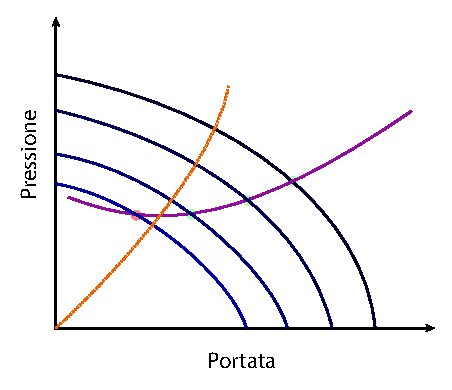
\includegraphics[width=.5\textwidth]{fig/foamer/ipr-tpr.eps}
    \caption{Schematizzazione dell'analisi nodale combinata alla portata critica di trascinamento}
    \label{fig:ipr-tpr}
\end{figure}


\section[Sollevamento artificiale per GDW]{Sistemi di sollevamento artificiale per il Gas Well Deliquification}
\sectionmark{Sollevamento artificiale per GDW}
L'industria del gas utilizza numerosi metodi per la rimozione di liquidi dai pozzi. Qui di seguito sono presentati i metodi più utilizzati e ormai consolidati nel tempo con particolare attenzione agli schiumogeni a cui è dedicata una sezione a parte. \textcite{oyewole2008artificial} classifica i sistemi di sollevamento artificiale in:
\begin{itemize}
    \item \textbf{a energia del giacimento}: qui definiti  a energia interna, i sistemi non aumentano direttamente l'energia del giacimento, bensì agiscono sui parametri che caratterizzano il trascinamento del liquido in pozzo;
    \item \textbf{a energia esterna}: sistemi a fondo pozzo che agiscono indipendentemente dall'energia residua del giacimento.
\end{itemize}
Le \textit{velocity string}, i compressori, i \textit{plunger} e gli schiumogeni sono sistemi di sollevamento artificiale a energia interna, pompe e iniezione di fluidi sono invece sistemi a energia esterna.

\subsection{Velocity string}
La \textit{velocity string} è praticamente un tubino di produzione con diametro inferiore rispetto a quello già presente in situ. Per produzione costante, il restringimento della sezione di produzione provoca un aumento della velocità del flusso in condotta e il superamento del valore della velocità critica. L'applicazione può avvenire su un tratto specifico del pozzo (\figref{fig:velocitystring-fixed}) oppure su tutta la sua lunghezza (\figref{fig:velocitystring-long}).

\begin{figure}[htbp]
\centering
    \subfloat[][Lunghezza fissa]
    {\makebox[0.4\textwidth]{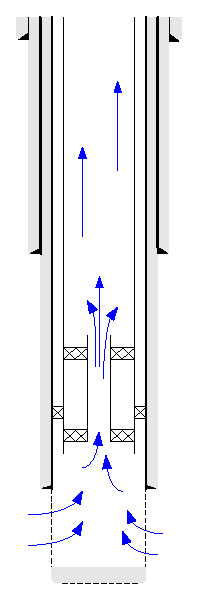
\includegraphics[width=.15\textwidth]{fig/foamer/velocitystring/velocitystring-fixed.eps}} \label{fig:velocitystring-fixed}} \quad
    \subfloat[][Su tutto il pozzo]
    {\makebox[0.4\textwidth]{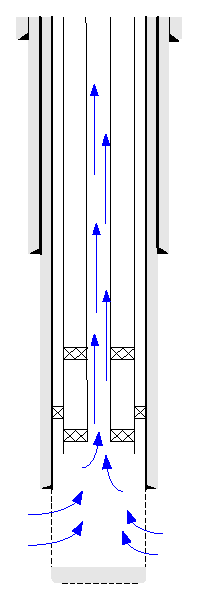
\includegraphics[width=.15\textwidth]{fig/foamer/velocitystring/velocitystring-long.eps}}\label{fig:velocitystring-long}}
    \caption{Schema di applicazione della velocity string \parencite{arachman2004liquid}} 
    \label{fig:velocitystring}
\end{figure}

L'installazione della \textit{velocity string} è generalmente molto economica rispetto ad altre sistemi di sollevamento artificiale, visto che l'applicazione può avvenire anche tramite \textit{coiled tubing}, prodotti tubolari continui a sezione limitata, fabbricati in lunghezza e avvolti attorno a una bobina di raccolta \parencite{international2014introduction}. Tuttavia la progettazione deve avvenire con particolare cautela, visto che il restringimento della sezione di produzione si traduce non solo in termini di aumento di velocità, ma anche di aumento delle perdite di carico per attrito. La \textit{velocity string} non è considerata una soluzione definitiva per il GWD, dal momento che il dimensionamento ideale del tubino di produzione ausiliario cambia con l'evoluzione delle condizioni del giacimento.

\subsection{Compressione}
Possono essere impiegati dei compressori in superficie per diminuire la pressione a testa pozzo. La modalità di compressione può essere a opera di un singolo compressore (\figref{fig:compressore}) o di un sistema di compressori posti in superficie. 

\begin{figure}[htbp]
    \centering
    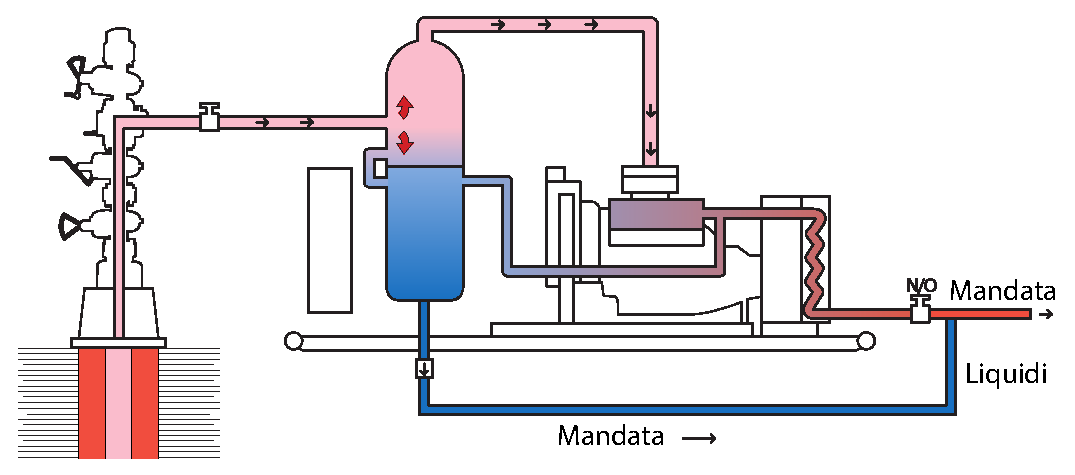
\includegraphics[width=\textwidth]{fig/foamer/compressore.eps}
    \caption{Layout semplificato del GasJack™, copressore singolo utilizzato per operazioni di compressione della testa pozzo \parencite{garner2009backside}}
    \label{fig:compressore}
\end{figure}

Una minore pressione a testa pozzo porta alla diminuzione dell'acqua proveniente da fenomeni di condensazione ma soprattutto all'aumento dell'afflusso di gas dal giacimento. L'aumento di portata è associato all'aumento della velocità del gas, raggiungendo così valori al di sopra della velocità critica. Il dimensionamento dell'impianto di compressione si basa sulla pressione di aspirazione e la pressione di mandata, ovvero dal rapporto di compressione. \'E importante tenere presente che una minima variazione delle pressioni di aspirazione o di mandata può aumentare in maniera significativa la potenza richiesta dal compressore. La compressione e la riduzione della pressione a testa pozzo sono generalmente le prime soluzioni impiegate per il sollevamento artificiale. L'installazione dei compressori può avvenire durante il ciclo di vita del pozzo senza evidenti segnali di \textit{liquid loading}: la diminuzione di pressione consente di lavorare in condizioni migliori, aumentando le performance generali e quindi la produzione di gas giornaliera. La compressione può anche considerarsi un sistema di sollevamento artificiale ausiliario: un compressore può interfacciarsi con altre soluzioni come agenti surfattanti, \textit{gas lift}, \textit{plunger}, \textit{beam pump}, ESP o \textit{velocity string}, aumentando in modo significativo le performance di \textit{liquid unloading}. La compressione può essere impiegata anche per avviare nuovamente un pozzo morto tramite un \textit{kick} indotto dal nuovo gradiente di pressione: soluzione alquanto inusuale, l'esperienza sul campo dice che solitamente una diminuzione di pressione non è sufficiente a garantire l'energia necessaria al pozzo per poter spiazzare anche parzialmente la colonna liquida presente.

\subsection{Plunger}
I plunger sono dei dispositivi installati all'interno del pozzo per la rimozione meccanica di liquidi e altri agenti contaminanti. Il \textit{plunger} è un pistone tuffante che viaggia liberamente dal fondo pozzo alla superficie, spinto da una pressione che deve essere sufficiente a trascinare sia il dispositivo che i fluidi accumulati. La produzione di gas con l'installazione di un \textit{plunger} risulta discontinua, legata alla ciclicità dello strumento che deve percorre in entrambe le direzioni tutta la lunghezza del pozzo. Come si può vedere nella \figref{fig:conventionalplunger} l'applicazione di un \textit{plunger} in pozzo richiede determinata strumentazione di superficie (valvole) e di fondo pozzo (\textit{plunger} e meccanismo a molla). Una tipica installazione convenzionale è organizzata nel seguente modo:

\begin{itemize}
    \item \textbf{\textit{bumper} a molla}, utile a ricevere il \textit{plunger} a fondo pozzo e evitare danni dovuti all'impatto a terra;
    \item \textbf{ricevitore di superficie}, blocca il \textit{plunger} una volta giunto in superficie e consente il deflusso del gas in condotta;
    \item \textbf{valvola motorizzata di superficie}, controllata elettronicamente, apre e chiude il pozzo quando necessario;
    \item \textbf{sensore elettronico di superficie}, si attiva quando il \textit{plunger} giunge in superficie;
    \item \textbf{controller elettronici}, con ciclicità impostata da operatore, gestisce tutte le operazioni di produzione e registra dati in continuo.
\end{itemize}

\begin{figure}[htbp]
    \centering
    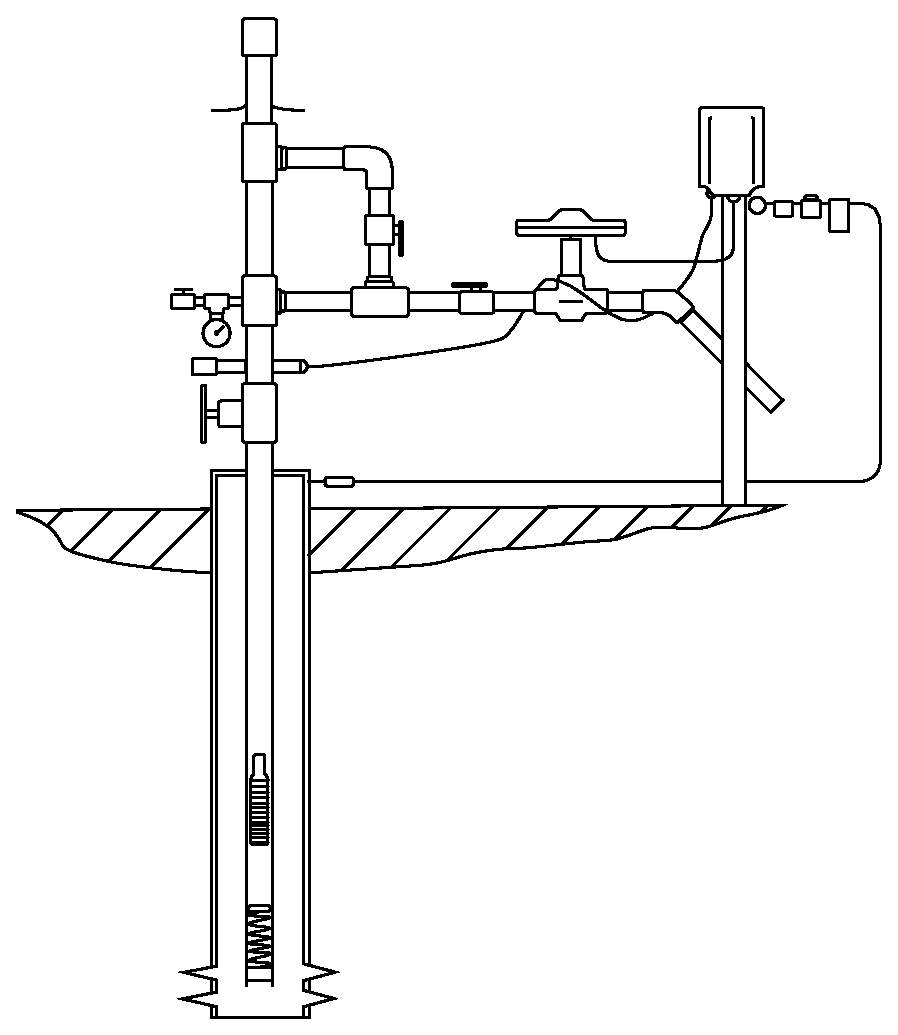
\includegraphics[width=0.6\textwidth]{fig/foamer/plunger-installation.eps}
    \caption{Tipica installazione di \textit{plunger} \parencite{lea2011gas}}
    \label{fig:plunger-installation}
\end{figure}

Come già detto, l'applicazione di un plunger convenzionale trasforma la produzione da continua a ciclica, caratterizzata quindi da \textit{shut-in} programmati per far tornare il \textit{plunger} alla posizione originaria e permettere al pozzo, in caso di bisogno, di raggiungere una pressione tale da poter trascinare il \textit{plunger} assieme alla colonna di fluido presente. La \figref{fig:conventionalplunger} mostra un generico ciclo di produzione convenzionale:
\begin{enumerate}
    \item[(a)] \textit{plunger} a fondo pozzo con liquido al di sopra, valvola di superficie chiusa;
    \item[(b)] apertura della valvola di superficie e risalita del \textit{plunger} assieme alla colonna liquida;
    \item[(c)] fase produttiva del pozzo in assenza di cadute di pressione dovute a \textit{liquid loading};
    \item[(d)] riaccumulo di fluido a fondo pozzo;
    \item[(e)] chiusura del pozzo e discesa del \textit{plunger} a fondo pozzo.
\end{enumerate}

\begin{figure}[htbp]
    \centering
    \subfloat[][]
    {\centering 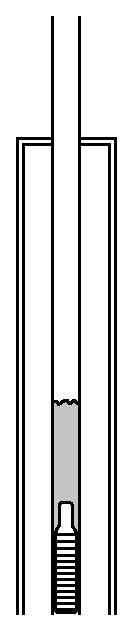
\includegraphics[height=.3\textheight]{fig/foamer/plunger-conventional/conventionalplunger-A.eps}} \label{fig:plunger-conventional-A} \qquad \qquad
    \subfloat[][]
    {\centering 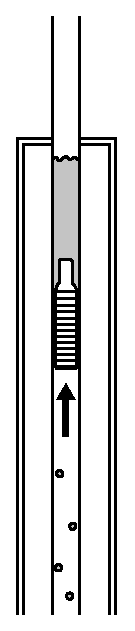
\includegraphics[height=.3\textheight]{fig/foamer/plunger-conventional/conventionalplunger-B.eps} \label{fig:plunger-conventional-B}}  \qquad \qquad
    \subfloat[][]
    {\centering 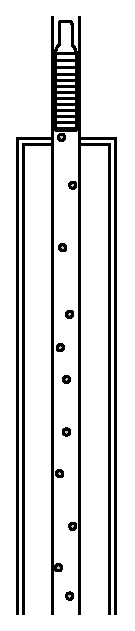
\includegraphics[height=.3\textheight]{fig/foamer/plunger-conventional/conventionalplunger-C.eps} \label{fig:plunger-conventional-C}} \qquad \qquad
    \subfloat[][]
    {\centering 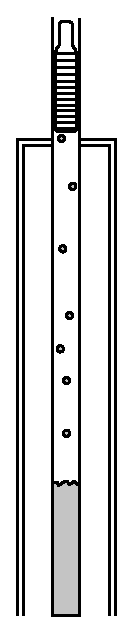
\includegraphics[height=.3\textheight]{fig/foamer/plunger-conventional/conventionalplunger-D.eps} \label{fig:plunger-conventional-D}} \qquad \qquad
    \subfloat[][]
    {\centering 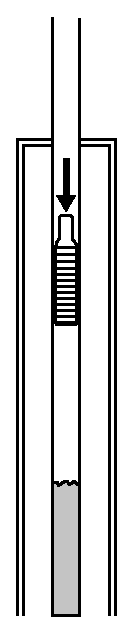
\includegraphics[height=.3\textheight]{fig/foamer/plunger-conventional/conventionalplunger-E.eps} \label{fig:plunger-conventional-E} }
    \caption{Ciclo di un plunger convenzionale}
    \label{fig:conventionalplunger}
\end{figure}

In commercio esistono varie tipologie di \textit{plunger} e variano a seconda della geometria e degli inserti installati sulla superficie esterna (e.g. spazzole per la pulizia del tubino di produzione). Negli ultimi anni sono nati nuovi sistemi definiti a ciclo libero o in continuo, che permettono la discesa senza interrompere la produzione. Numerosi sono i brevetti e i prodotti che offrono \textit{plunger-lift} in continuo: possono essere dotati di una valvola interna (e.g. Weatherford RapidFlo™, FB FreeCycle™ o McClain™) oppure a due pezzi (e.g. Peacemaker™, composto da una sfera e un manicotto). La \figref{fig:plunger} mostra alcune tipologie presenti sul mercato.\\
L'applicazione di \textit{plunger} in pozzo per il sollevamento artificiale richiede un investimento iniziale relativamente basso, ma dei costi operativi che possono incidere col tempo e portare a un aumento imprevisto del costo di produzione del gas. Gli investimenti iniziali indiretti possono però incidere fortemente sulla scelta del \textit{plunger}: la variazione dei volumi di gas e liquido rende necessaria una nuova valutazione circa il dimensionamento degli impianti di trattamento a valle del pozzo, i costi iniziali possono essere quindi legati per esempio all'installazione di un nuovo separatore.

\begin{figure}[htbp]
\centering
    \subfloat[][A spirale]
    {\makebox[0.2\textwidth]{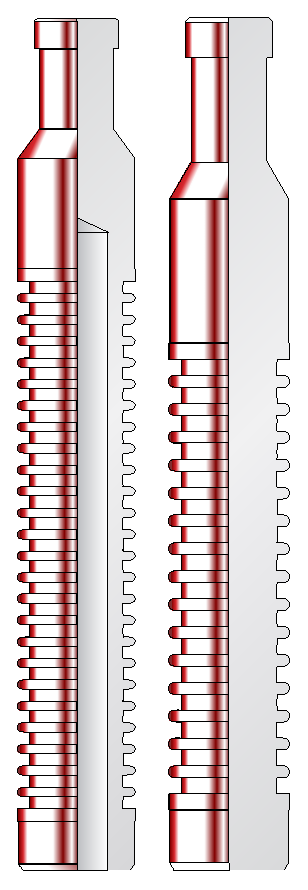
\includegraphics[height=.25\textheight]{fig/foamer/plunger/plunger-spiral.eps}} \label{fig:plunger-spiral}} \quad
    \subfloat[][T-pad]
    {\makebox[0.2\textwidth]{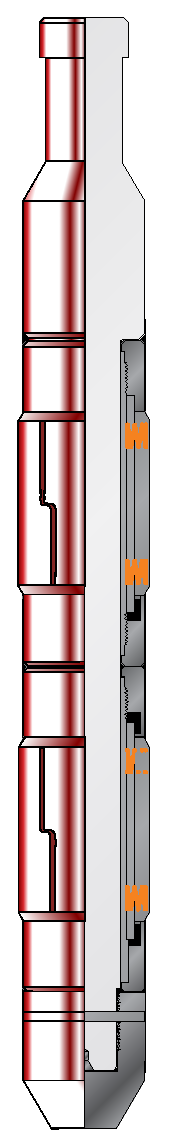
\includegraphics[height=.25\textheight]{fig/foamer/plunger/plunger-tpad.eps}} \label{fig:plunger-tpad}}  \quad
    \subfloat[][A spazzole fisse]
    {\makebox[0.2\textwidth]{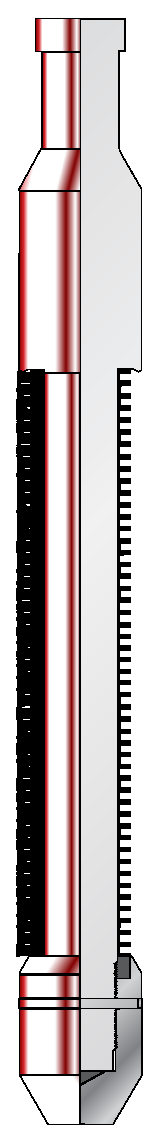
\includegraphics[height=.25\textheight]{fig/foamer/plunger/plunger-fixedbrush.eps}} \label{fig:plunger-fixedbrush}} \quad
    \subfloat[][RapidFlo™]
    {\makebox[0.25\textwidth]{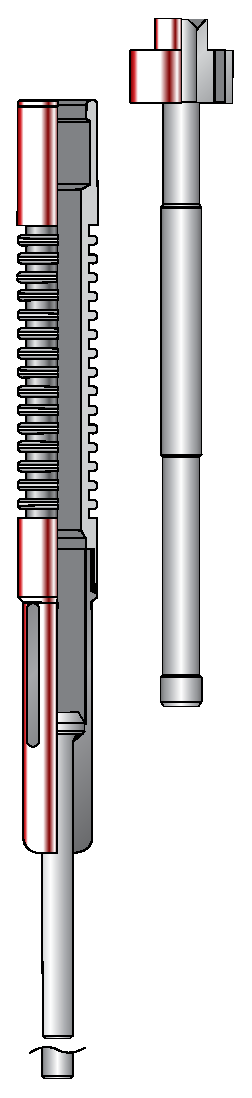
\includegraphics[height=.25\textheight]{fig/foamer/plunger/plunger-rapidflo.eps}} \label{fig:plunger-rapidflo} }
\caption{Principali tipologie di \textit{plunger} proposte da Weatherford \parencite{weatherford2008brochure}}
\label{fig:plunger}
\end{figure}

\subsection[Altri sistemi per GWD]{Altri sistemi di sollevamento artificiale per deliquification}
Alcune tecnologie per l'attenuazione del battente idrostatico in pozzo nascono da applicazioni pensate in origine per il sollevamento artificiale di giacimenti a olio. Questi sistemi sono stati riadattati per il trascinamento dell'acqua a fondo pozzo o per agevolare l'afflusso del gas in pozzo. I sistemi presentati nel paragrafo corrente sono tutti a energia esterna.
\paragraph{Gas lift}
Il \textit{gas lift} per \textit{deliquification} consiste nell'iniezione di gas da una fonte esterna al pozzo a una certa profondità. Nel campo dell'olio il gas iniettato a fondo pozzo diminuisce la densità dell'olio, facilitando così il flusso in condotta. In questo caso viene fatto fluire gas a fondo pozzo sia per diminuire la densità della colonna idrostatica, sia per aumentare la produzione di gas effettiva e quindi l'efficacia di trascinamento della colonna da parte della corrente gassosa. Questo sistema gode il vantaggio di non provocare significative variazioni alle condizioni di produttività  del pozzo e riesce a lavorare anche in perforazioni deviate. L'applicazione purtroppo dipende fortemente dalla presenza di una sorgente di gas ad alta pressione, rappresentata da un pozzo nella zona limitrofe o l'installazione di un compressore, a cui però sono associati alti costi operativi. Per di più il tubino di produzione deve essere progettato per sopportare l'aumento di pressione che si ha in condotta e l'impiego di gas ad alta pressione può portare facilmente a problemi di congelamento e creazione di idrati.
\paragraph{Sistemi di pompaggio}
Le pompe petrolifere o a cavalletto (\textit{Beam Pump} o BP, impiegate in modo massiccio per il sollevamento artificiale per giacimenti a olio, rappresentano il sistema di pompaggio più comune anche nel GWD. Generalmente i sistemi di pompaggio spingono la colonna idrostatica lungo il tubino di produzione (o un tubino ausiliario, come un \textit{coiled tubing} installato a posteriori) e il gas prodotto viene fatto fluire nell'annulus. Altri sistemi di pompe utilizzate anche in questo campo sono le pompe elettriche sommerse (\textit{Electrical Submersible Pump},   ESP), pompe a cavità progressiva (\textit{Progressing Cavity Pump}, PCP) e pompe idrauliche (a pistone o \textit{jet pump}). Le pompe vengono generalmente impiegate quando la pressione a fondo pozzo è relativamente bassa e quando il rapporto gas/liquido non è sufficiente da garantire lo spiazzamento della colonna idrostatica tramite i sistemi a energia interna. Le pompe non possono operare in presenza di gas, perciò vanno opportunamente collocate al di sotto degli spari, in modo da ottenere una buona separazione del liquido dal gas. La vita media delle pompe dipende fortemente dagli agenti di erosione, è importante capire se la produzione di liquidi e gas comporta anche la produzione di sabbia.

\section{Schiumogeni}
L'impiego di schiumogeni nell'industria petrolifera è vario e ormai consolidato nel tempo. Come visibile in \tabref{tab:surfactantapplications} i tensioattivi sono impiegati in tutte le fasi di recupero del greggio e nell'industria di processo, dalle perforazioni, iniezioni in giacimento, produzione, al trasporto in condotta onshore e offshore.

\begin{table}[htbp]
    \small
    \centering
    \caption{Alcuni esempi di applicazioni di tensioattivi nell'industria petrolifera \parencite{schramm2006emulsions}.}
    \label{tab:surfactantapplications}
\begin{tabular}{p{.8\textwidth}p{.1\textwidth}}
\hline
{\bf Applicazione}                                                         & {\textbf{Fasi}}           \\ \hline
Fluidi di perforazione con schiume                                         & G/W                    \\
Fluidi di stimolazione e fratturazione con schiume                         & G/W                    \\
Fluidi acidificanti con schiume                                            & G/W                    \\
Recupero di olio freddo e pesante tramite schiume                          & G/O                    \\
Schiume di processo della flottazione dell'olio                            & G/O                    \\
Schiume antincendio                                                        & G/W                    \\
Emulsioni per olio pesante in condotta                                     & O/W                    \\
Emulsioni per la stimolazione pozzo                                        & O/W                    \\
Flottazione di miscele a olio e sabbie bituminose                          & O/W                    \\
Fluidi di perforazione emulsionati (fanghi a base olio)                    & W/O                    \\
Emulsione di catrame e bitumi                                              & O/W                    \\
Emulsioni in situ per EOR                                                  & O/W                    \\
Emulsione di carburanti di trasporto (70\% olio pesante)                   & O/W                    \\
Schiume per il controllo della mobilità del gas                            & G/W                    \\
Sospensioni per fluidi (fanghi) di perforazione                            & S/W                    \\
Sospensioni per fratturazione idraulica e stimolazione del pozzo           & S/W                    \\
Impasti cementizi in pozzo                                                 & S/W                    \\
Solidi di produzione a testa pozzo nel recupero primario dell'olio pesante & S/W                    \\ \hline
\end{tabular}
\end{table}

I tensioattivi sono utilizzati anche in pozzo per mitigare i fenomeni di \textit{liquid loading} e la tecnica ha ormai acquisito notevole importanza nel GWD. I tensioattivi sono introdotti in pozzo in tre modi:
\begin{itemize}
    \item \textit{\textbf{stick}}: barre solide di sapone introdotte lungo il tubino di produzione senza la necessità di interrompere la produzione;
    \item \textbf{schiumogeni in-batch}: viene chiuso il pozzo e viene pompato lungo il tubino di produzione un certo volume di surfactanti in soluzione salina, per poi riaprire il pozzo il giorno dopo;
    \item \textbf{schiumogeni in continuo}: una \textit{capillary string}, collegata a una pompa dosatrice, viene calata lungo il pozzo fino all'altezza degli spari, lo schiumogeno liquido viene iniettato durante la produzione di gas.
\end{itemize}
 Gli \textit{stick} sono facili da utilizzare, non comportano modifiche di impianto e rappresentano il metodo più economico. Tuttavia interessano solo la parte superiore della colonna liquida e rimuovono parzialmente l'acqua a fondo pozzo; inoltre, essendo solubili in acqua, non agiscono in modo appropriato in presenza di idrocarburi condensati sull'interfaccia gas-liquido \parencite{bolding2007resurrecting}. Nel seguente paragrafo si farà riferimento ai soli \textit{defoamer}, descrivendo i principi e le procedure operative per il sollevamento artificiale tramite tensioattivi liquidi.
 
\subsection{Tensioattivi}
I tensioattivi, surfactanti o agenti attivi di superficie sono composti organici composti al massimo da un gruppo, testa, liofilo e un gruppo, coda, liofobico \figref{fig:sls}. Si parla di testa idrofila e coda idrofoba se il solvente nel quale deve essere utilizzato il tensioattivo è acqua o a base acqua. In termini chimico-fisici la struttura di un surfactante è costituita da un gruppo polare e da un gruppo apolare . La \figref{fig:sls} mostra un esempio di struttura chimica di un tensioattivo con in evidenza il gruppo polare e apolare.

\begin{figure}[htbp]
    \centering
    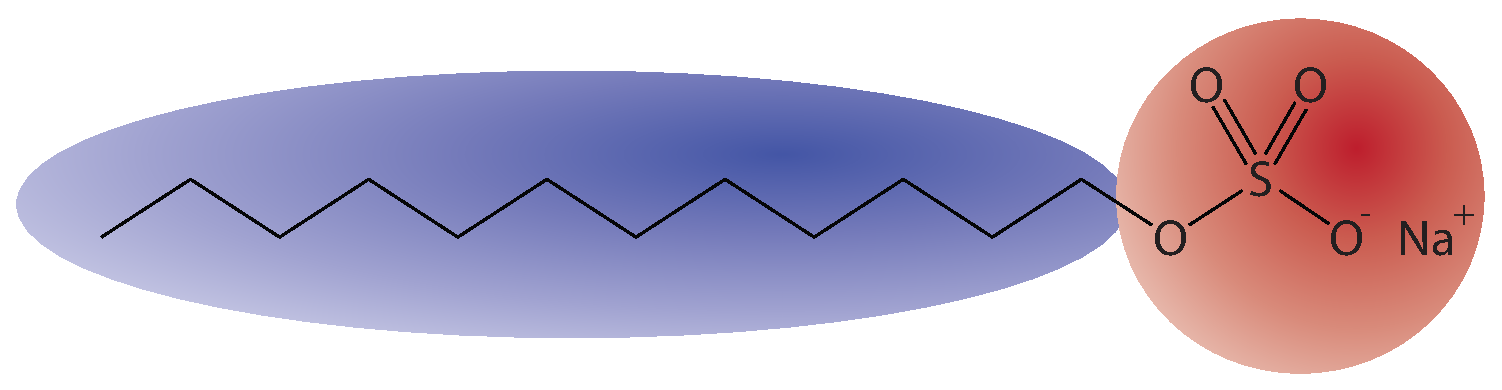
\includegraphics[width=.8\textwidth]{fig/foamer/sls.eps}
    \caption{Laurilsolfato di sodio, tensioattivo anionico utilizzato in molte famiglie di prodotti domestici. La catena a 12 atomi di carbonio rappresenta il gruppo apolare (in blu) mentre il gruppo solfato associato allo ione sodio rappresenta il gruppo polare (in viola).}
    \label{fig:sls}
\end{figure}

I surfactanti sono classificati in base alla carica del gruppo polare (\figref{fig:surfactants-classification}):
\begin{itemize}
    \item \textbf{anionici}: in genere sali costituiti da lunghe catene con atomi di carbonio che terminano con un gruppo carbossilato, solfonato o fosfato;
    \item \textbf{cationici}: sali di cui è importante la parte positiva, costituita da lunghe catene di atomi di carbonio terminanti con un gruppo ammonico;
    \item \textbf{non ionici}: alcoli a lunga catena, come i derivati poliossietilenici degli acidi grassi;
    \item \textbf{anfoteri} o \textbf{zwitterionici}: tensioattivi anionici in ambiente alcalino, tensiattivi cationici in ambiente acido.
\end{itemize}

\begin{figure}[htbp]
    \centering
    \subfloat[][Anionici]
    {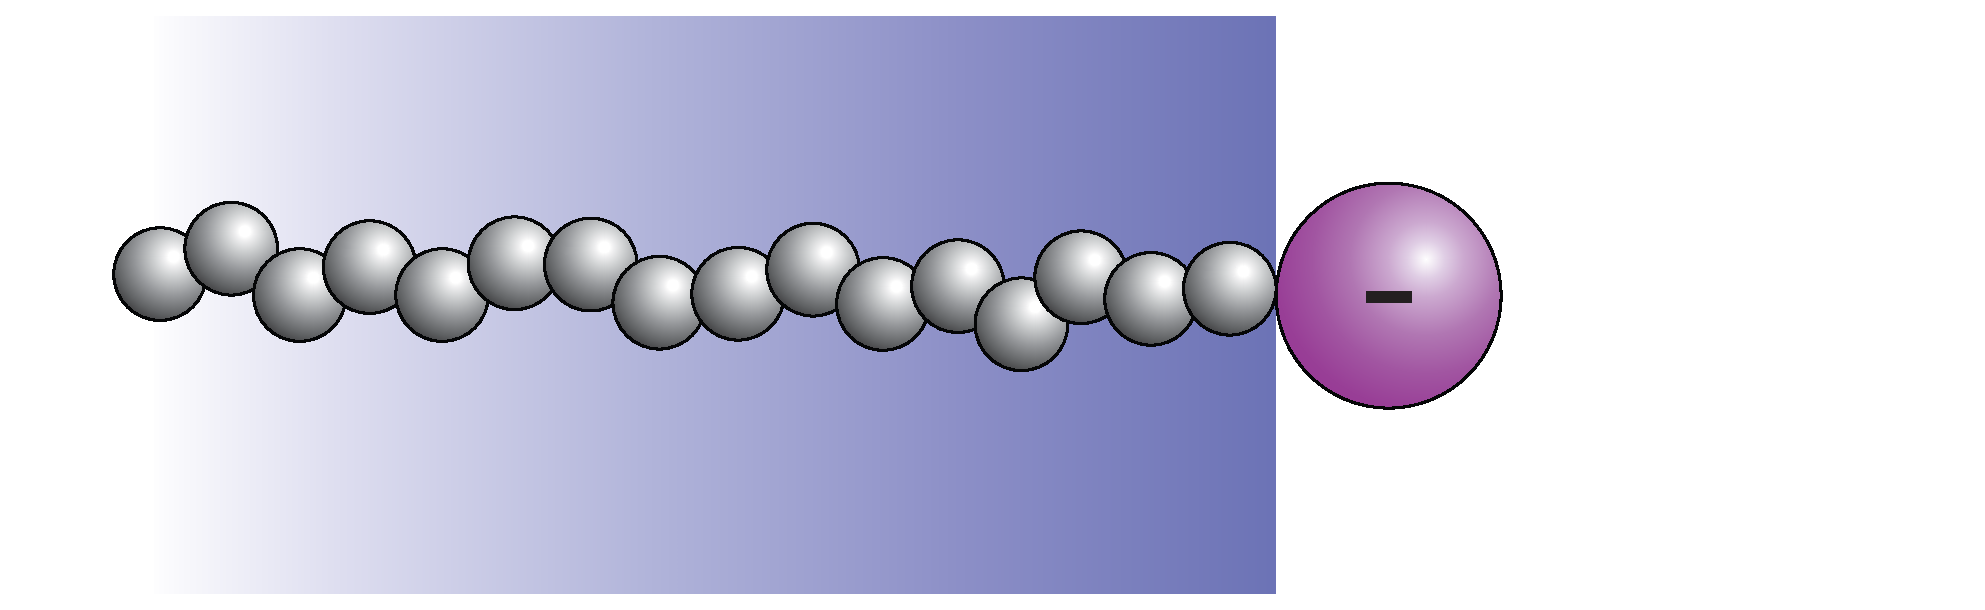
\includegraphics[width=.45\textwidth]{fig/foamer/surfactants-classification/anionic.eps} \label{fig:anionic}} \quad
    \subfloat[][Cationici]
    {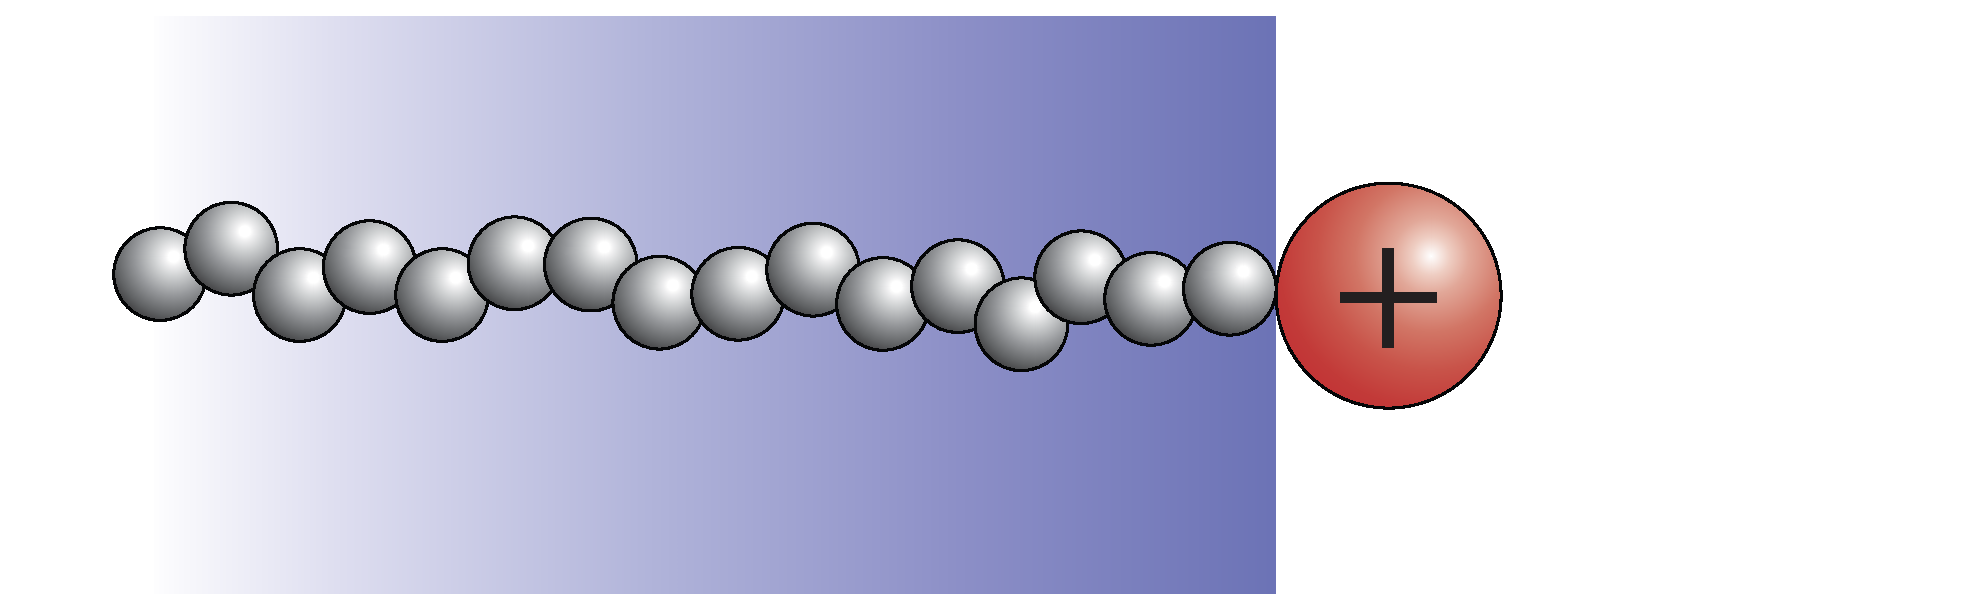
\includegraphics[width=.45\textwidth]{fig/foamer/surfactants-classification/cationic.eps} \label{fig:cationic}}  \\
    \subfloat[][Anfoterici]
    {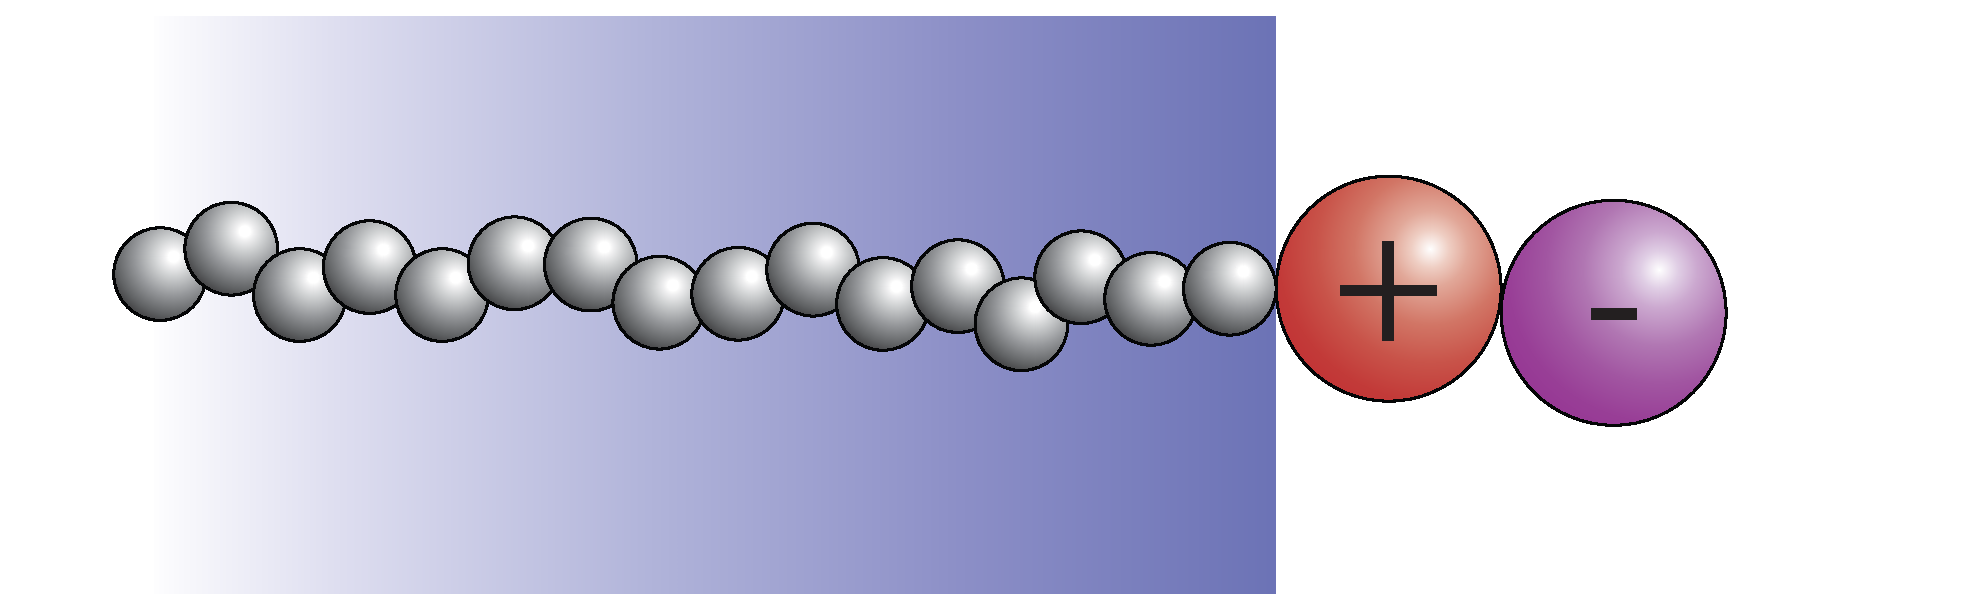
\includegraphics[width=.45\textwidth]{fig/foamer/surfactants-classification/anphoteric.eps} \label{fig:anphoteric}}  \quad
    \subfloat[][Non ionici]
    {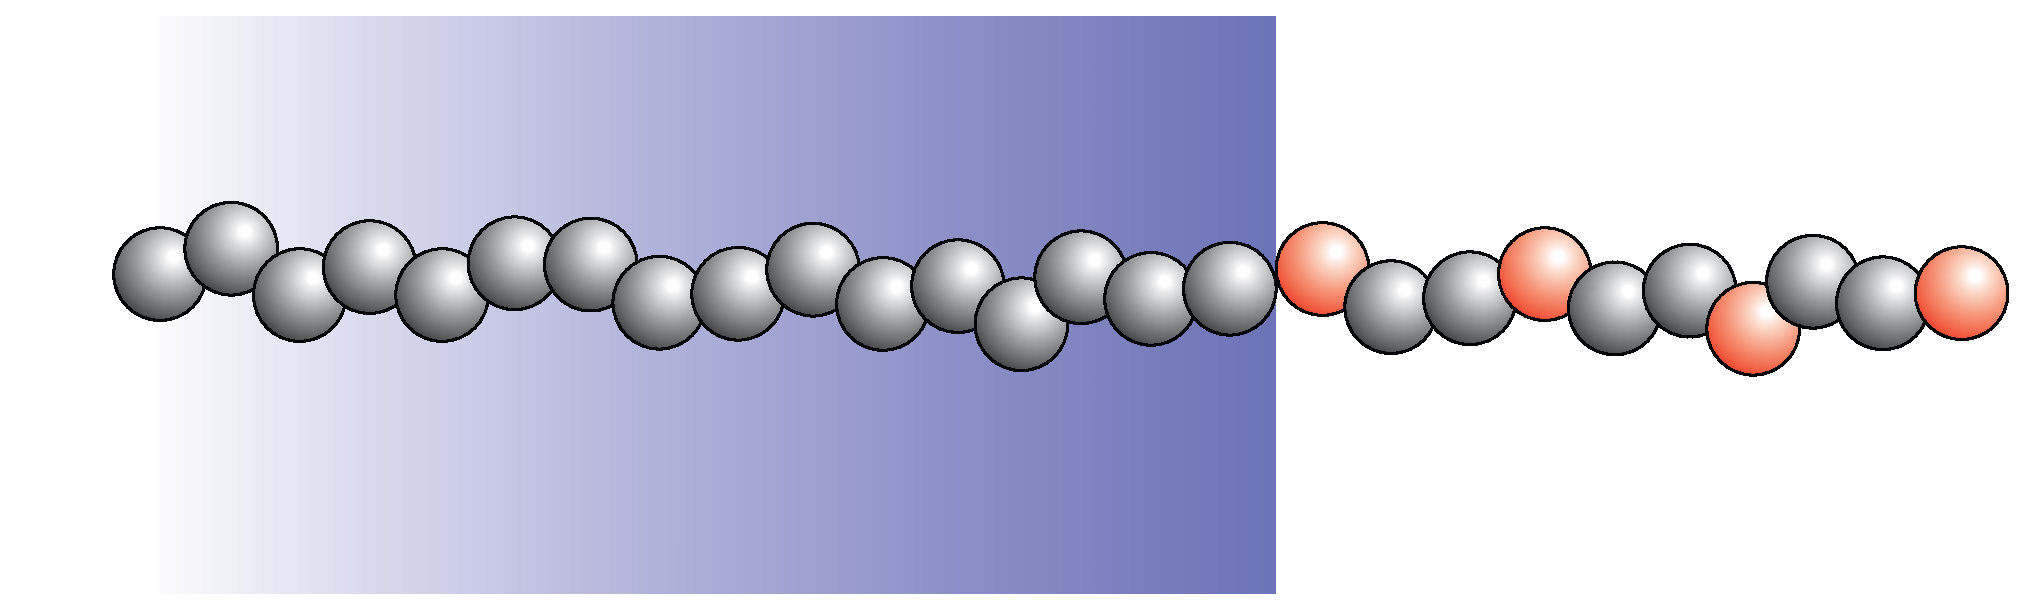
\includegraphics[width=.45\textwidth]{fig/foamer/surfactants-classification/nonionic.eps} \label{fig:nonionic}} 
\caption{Classificazione dei tensioattivi in base alla carica del gruppo polare.}
\label{fig:surfactants-classification}
\end{figure}

Due fenomeni derivano dalla presenza di un gruppo polare e apolare all'interno della stessa molecola: adsorbimento e aggregazione.\\
Si consideri un volume d'acqua a contatto con aria dove vengono disciolti dei tensioattivi. I surfactanti, in prossimità della superficie di contatto delle due fasi, si orientano in modo tale che il gruppo polare sia adsorbito dalla fase liquida e il gruppo apolare permanga nella fase gassosa. Tale adsorbimento porta alla diminuzione dell'energia libera di Gibbs o entalpia libera, quindi alla riduzione della tensione superficiali tra le due fasi. Allo stesso modo i tensioattivi possono diminuire la tensione superficiale dell'acqua a contatto con una generica fase olio o di un solido, aumentando la bagnabilità di quest'ultimo.

Un altro modo per limitare il contatto del gruppo apolare con l'acqua è la creazione di strutture bi- o tridimensionali, capaci di racchiudere i gruppi apolari internamente e mettendo a contatto con l'acqua i gruppi polari (\figref{fig:micelle}). Queste strutture sono definite micelle, sono il frutto dei fenomeni di aggregazione dei tensioattivi e possono avere forma lamellare (in questo caso i surfactanti sono molecole anfifiliche o anfifobiche), sferica o cilindrica.  Tali aggregati supramolecolari tendono a crearsi una volta superato una certa concentrazione del surfactante in soluzione, definita concentrazione micellare critica (CMC). La complessità di tali strutture dipende dalla concentrazione in acqua e dalla specie chimica dell'agente attivo di superficie.

\begin{figure}[htbp]
    \centering
    
\includegraphics[width=.5\textwidth]{fig/foamer/micelle.eps}
    \caption{Sezione parziale di una micella anionica, il layer compatto negativo generato dall'orientamento del gruppo polare del tensioattivo è circondato dalla fase acqua  \parencite{attwood2012fasttrack}.}
    \label{fig:micelle}
\end{figure}

\subsection{Schiuma}
Viene definita schiuma una dispersione stabile di gas in un liquido. Se si introduce un flusso di aria all'interno di un liquido, le bolle così prodotte assumono una forma sferica. Poiché l'aria ha densità minore dell'aria queste tenderanno a salire in superficie. Se il liquido in questione è privo di surfactanti in soluzione, le bolle sono stabili limitatamente e esplodono spontaneamente (\figref{fig:foam-stability-nonsurfactants}). Non è possibile quindi creare una schiuma stabile in un liquido senza la presenza di surfactanti. In liquidi con tensioattivi in soluzione, le bolle sono rese stabili grazie all'azione degli agenti attivi di superficie, che creano un film attorno alle bolle di gas. Una volta giunte in superficie, le bolle presentano un doppio strato o doppio film di tensioattivi sulla superficie (\figref{fig:foam-stability-surfactants}).

\begin{figure}[htbp]
    \centering
    \subfloat[][Liquidi senza tensioattivi]
    {
\includegraphics[height=.222\textheight]{fig/foamer/foam-stability/non-surfactants.eps} \label{fig:foam-stability-nonsurfactants}} \quad
    \subfloat[][Liquidi con tensioattivi]
    {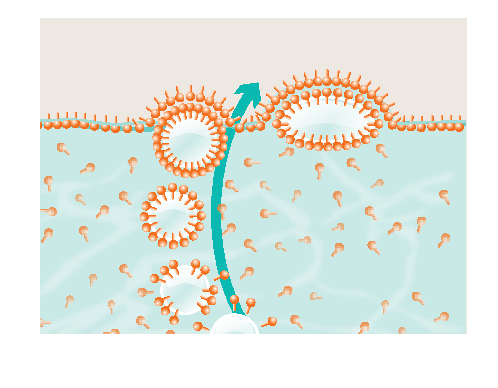
\includegraphics[height=.222\textheight]{fig/foamer/foam-stability/surfactants.eps} \label{fig:foam-stability-surfactants}}
    \caption{Insufflazioni nel liquido e generazione delle bolle d'aria \parencite{tego2014brochure}.}
    \label{fig:surfactants-stability}
\end{figure}

Le bolle appena generate all'interno del liquidi, dalle piccole dimensioni e pressoché identiche, sono definite microbolle; le bolle visibili sulla superficie sono definite macrobolle. In un primo momento la schiuma generata è ricca in liquidi, le bolle hanno configurazione sferica e sono stabili grazie a spesse lamelle liquide a doppio strato di tensioattivo. Con il tempo la forza di gravità agisce sulla fase liquida della schiuma, che defluisce così verso il basso: il processo è definito drenaggio per gravità. Si distinguono quindi due configurazioni di schiuma, prima e dopo il processo di drenaggio (\figref{fig:lamella}):
\begin{itemize}
    \item \textbf{schiuma bagnata}: bolle sferiche e contributo importante della fase liquida;
    \item \textbf{schiuma asciutta}: struttura poliedrica dettata dalla bassa presenza di liquido e caratterizzata da lamelle di schiuma molto elastiche.
\end{itemize}

\begin{figure}[htbp]
    \centering
    \includegraphics[width=.6\textwidth]{fig/foamer/lamella.eps}
    \caption{Struttura della schiuma e stabilizzazione della lamella a opera dei surfactanti \parencite{tego2014brochure}.}
    \label{fig:lamella}
\end{figure}

Il processo di drenaggio non è però sufficiente ad abbattere la schiuma. Si raggiunge un punto in cui il drenaggio non è più possibile poiché le alte concentrazioni di tensioattivi sono tali che le forze di repulsione elettrostatica e sterica impediscono un'ulteriore contrazione delle lamelle. La schiuma è quindi definita stabile quando si instaura uno stato di equilibrio tra il drenaggio per gravità e le forze di repulsione tra molecole.
Le sottili lamelle di schiuma, oltre ad essere stabili, sono molto elastiche. Un aumento della superficie delle lamella, provocato dalla deformazione della bolla, porta alla riduzione locale della concentrazione di surfactanti e di conseguenza a un aumento locale della tensione superficiale della lamella stessa. L'elasticità di Gibbs-Marangoni consente quindi alla schiuma, se sollecitata dall'esterno, di tornare alla configurazione geometrica iniziale.

\subsection{Antischiuma}
Gli antischiuma o \textit{defoamer} sono agenti chimici capaci di penetrare la lamella della schiuma, destabilizzando la struttura della bolla per farla così esplodere. Le caratteristiche principali di un buon antischiuma sono:
\begin{itemize}
    \item insolubilità nella soluzione generatrice di schiuma;
    \item bassa tensione superficiale;
    \item coefficiente di penetrazione (\(E\)) positivo;
    \item coefficiente di espansione (\(S\)) o coefficiente di \textit{bridging} positivo oppure caratteristiche di \textit{dewetting}.
\end{itemize}

L'insolubilità del \textit{defoamer} non deve essere assoluta: l'antischiuma deve pur sempre essere sufficientemente compatibile con il mezzo da trattare. 
Come già detto il \textit{defoamer} deve penetrare la lamella in modo da disgregare le bolle della schiuma. Un prerequisito fondamentale è quindi la capacita di penetrare il film di tensioattivi. La capacità penetrante dell'antischiuma è espressa fisicamente dal coefficiente di penetrazione \(E\):
\[E = \sigma_{L/G} + \sigma_{L/D} + \sigma_{D/G} \label{eq:penetration} \]
dove \(\sigma\) rappresenta la tensione superficiale e fa riferimento alla fase liquido-gas (\(L/G\)), liquido-defoamer (\(L/D\)) e \textit{defoamer}-gas (\(D/G\)). Solo se \(E\) è positivo, l'antischiuma è capace di permanere sulla parete della lamella, altrimenti rimane all'interno della soluzione liquida. Giunta sul film di surfactanti,  la gocciolina di \textit{defoamer} può espandersi su tutta la superficie della lamella, formando così delle lenti. Il risultato è una diminuzione della stabilità e flessibilità della lamella che porta così alla disgregazione della bolla. Il processo di espansione porta allo scorrimento del fluido nella lamella lungo le direzioni di espansione del \textit{defoamer}. Il fenomeno è conosciuto come flusso di Marangoni e provoca un restringimento dello strato della lamella, destabilizzando ulteriormente la struttura della bolla. Il coefficiente di espansione \(S\) esprime le capacità espandenti dell'antischiuma:
\[S = \sigma_{L/G} - \sigma_{L/D} - \sigma_{D/G} \label{eq:spreading} \]

\begin{figure}[htbp]
    \centering
    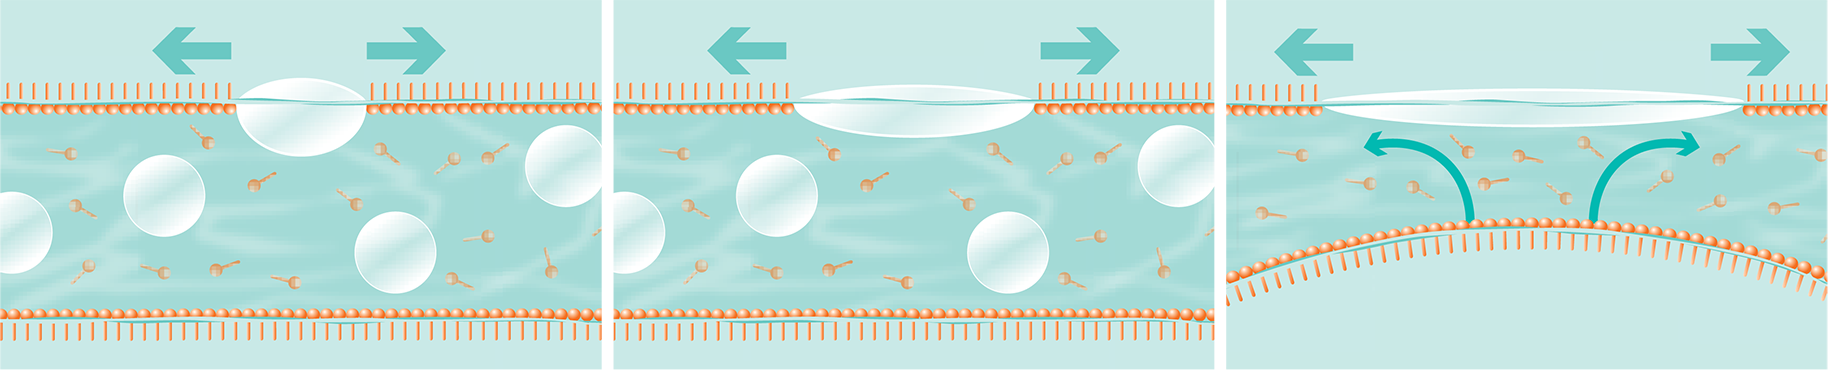
\includegraphics[height=.11\textheight]{fig/foamer/penetration.png}
    \caption{Penetrazione e espansione del \textit{defoamer} sul film di tensioattivi \parencite{tego2014brochure}.}
    \label{fig:penetration}
\end{figure}

I \textit{defoamer} con insufficienti capacità espandenti possono trattare la schiuma tramite il processo di \textit{bridging}. Requisito fondamentale è la capacità dell'antischiuma di penetrare sia il film esterno della lamella, quindi un coefficiente di penetrazione positivo, sia il film interno. 

\begin{figure}[htbp]
    \centering
    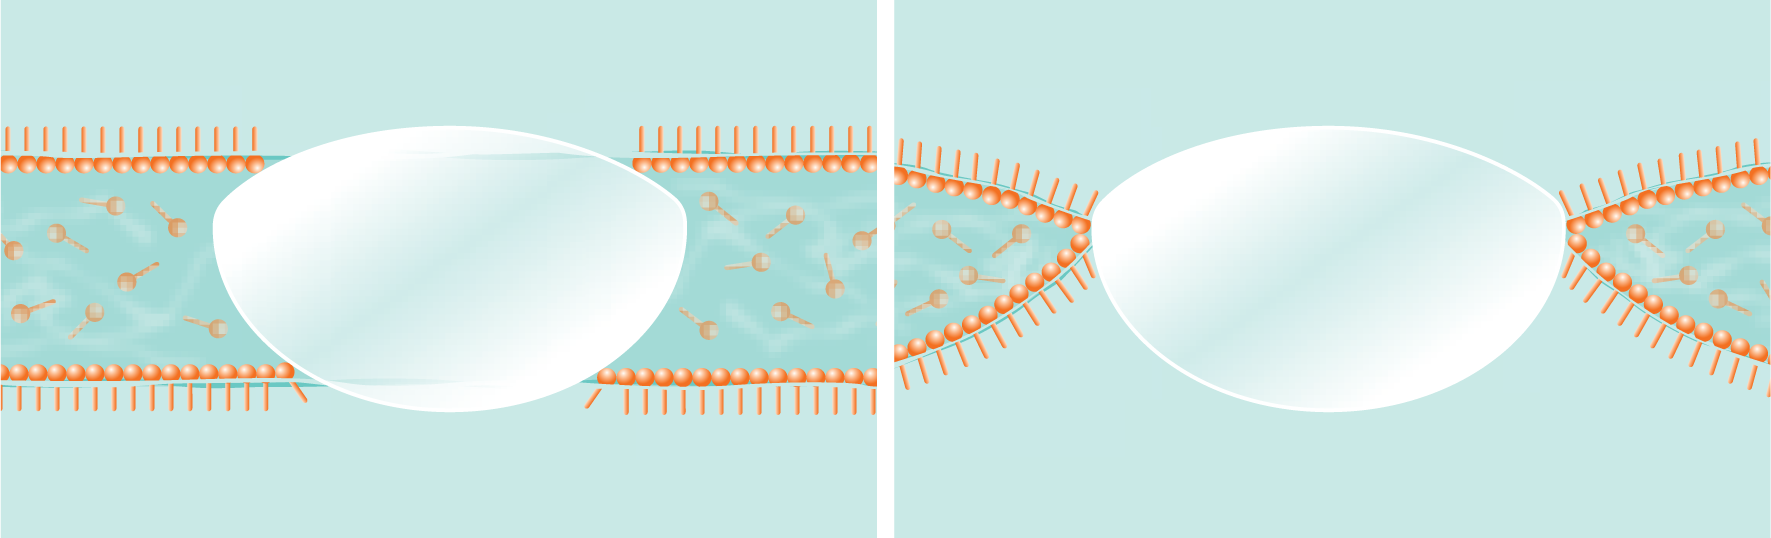
\includegraphics[height=.11\textheight]{fig/foamer/bridging.png}
    \caption{Processo di bridging del \textit{defoamer} sul film di tensioattivi \parencite{tego2014brochure}.}
    \label{fig:bridging}
\end{figure}

Ciò è possibile se la lamella è sufficientemente ristretta grazie al drenaggio per gravità oppure se le bolle sono sufficientemente grandi per via del fenomeno di coalescenza. Raggiunta l'altra parete della lamella, la rottura della lamella può avvenire per allungamento o \textit{dewetting}. I due meccanismi sono possibili se il coefficiente di \textit{bridging} \(B\) è positivo:
\[B = (\sigma_{L/G})^2 + (\sigma_{L/D})^2 - (\sigma_{D/G})^2 \label{eq:bridging} \]

Se l'antischiuma agisce tramite \textit{dewetting}, la soluzione liquida non riesce a entrare totalmente in contatto con le goccioline di \textit{defoamer}. Di conseguenza, il fenomeno di \textit{dewetting} porta al collasso delle bolle generate dai tensioattivi. Anche gli agenti solidi portano al fenomeno di \textit{dewetting}.
Se il processo di rimozione di schiuma avviene tramite l'allungamento delle lamelle, le goccioline di antischiuma agiscono sul punto più debole della lamella per portarla alla lacerazione e quindi alla destabilizzazione della configurazione totale della schiuma.

\begin{figure}[htbp]
    \centering
    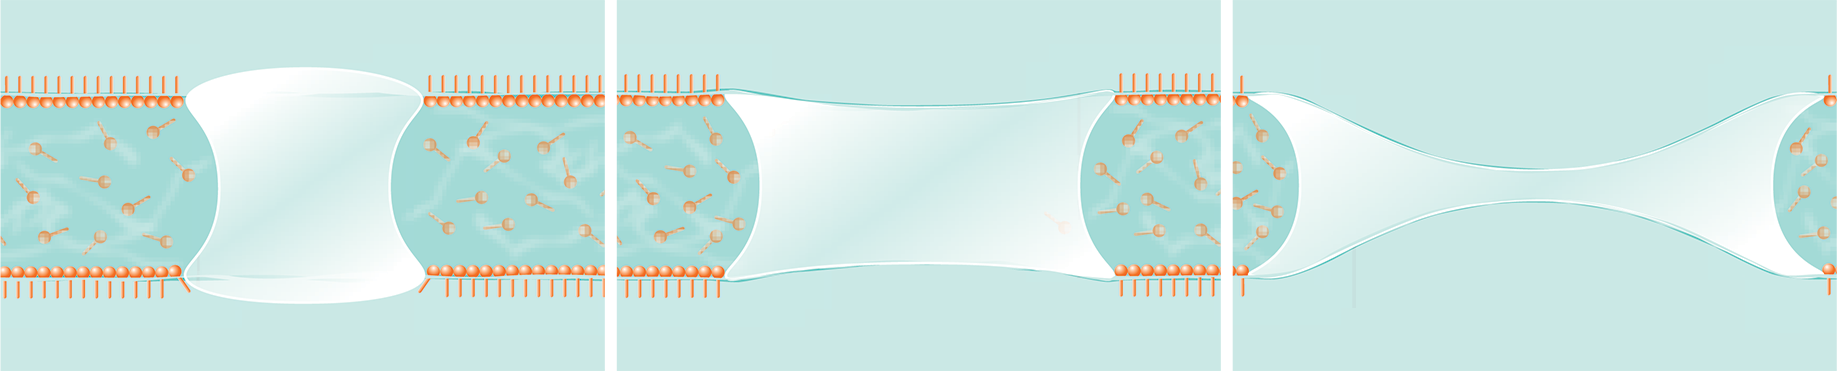
\includegraphics[height=.11\textheight]{fig/foamer/dewetting.png}
    \caption{Processo di dewetting del \textit{defoamer} sul film di tensioattivi \parencite{tego2014brochure}.}
    \label{fig:dewetting}
\end{figure}

Attualmente le classi di \textit{defoamer} in commercio sono:
\begin{itemize}
    \item \textbf{siliconici}: i polisilossani e suoi affini (e.g. polidimetilsilossani) appartengono al gruppo di antischiuma più comunemente utilizzati, sono polimeri costruiti su un gruppo silossano, dove al centro della molecola si alternano atomi di silicio e ossigeno, hanno grandi capacità di espansione e efficacia a largo spettro;
    \item \textbf{oli minerali}: generalmente idrocarburi alifatici e non aromatici per motivi ambientali, queste molecole apolari hanno buone capacità di espansione, hanno problemi in ambienti molto alcalini e ad alte temperature;
    \item \textbf{a base di olio vegetale}: o anche definiti antischiuma VOC-free, presentano proprietà molto simili agli oli minerali con il vantaggio di utilizzare una risorsa rinnovabile, solitamente con l'aggiunta di siliconi e cere sintetiche;
    \item \textbf{a base di polimeri}: possono essere acidi grassi modificati, polieteri o ammine modificate, la polarità di queste molecole può essere cambiata lavorando la struttura chimica e, grazie alla loro grande compatibilità, sono impiegati laddove non è possibile impiegare altri \textit{defoamer}.
\end{itemize}

\section[Applicazione di schiumogeni per GWD]{Applicazioni di schiumogeni per il Gas Well Deliquification} \label{section:foamer-ll}
L'applicazione di surfactanti o schiumogeni in pozzi affetti da \textit{liquid loading} permette di avviare la produzione anche se la velocità del fluido è minore della normale velocità critica e evita l'innalzamento della colonna idrostatica a fondo pozzo. Si consideri la \eqref{eq:turnerwc}: \textcite{turner1969analysis} fornisce il valore della velocità critica in funzione della densità dei fluidi e della tensione superficiale fra le due fasi. L'impiego di surfactanti permette di ridurre la tensione superficiale tra i liquidi e l'acqua, così come la densità dell'acqua, trasformata in parte in schiuma. \textcite{campbell2001corrosion} definisce in via teorica che la tensione superficiale possa essere ridotta da 60 dyne/cm a 30 dyne/cm e che la densità della schiuma possa attestarsi al 20\% della densità originaria della fase liquida (\figref{fig:campbell}). Da questi valori si può facilmente calcolare che i tensioattivi permettono di ridurre la portata critica di un pozzo affetto da \textit{liquid loading} di circa il 30\%. \textcite{wittfeld2015foam} conferma questi dati sperimentalmente e propone una riduzione del valore di portata critica del 33\%, con picchi del 45\% su breve periodo.

\begin{figure}[htbp]
    \centering
    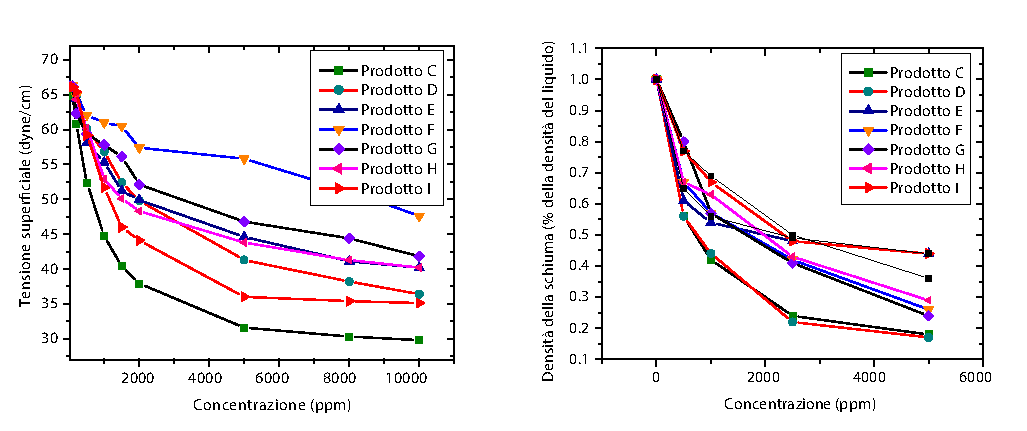
\includegraphics[width=\textwidth]{fig/foamer/campbell.eps}
    \caption{Tensione superficiale e densità della schiuma in funzione della concentrazione in acqua per tensioattivi attualmente disponibili sul mercato \parencite{campbell2001corrosion}.}
    \label{fig:campbell}
\end{figure}

Le procedure operative e i dati sperimentali qui esposti sono presi interamente dal "\citetitle{wittfeld2015foam}" di \textcite{wittfeld2015foam} a cura della \textit{Nederlandse Aardolie Maatschappij} (NAM, letteralmente \textit{Compagnia Petrolifera Olandese}). Attualmente i fenomeni di \textit{liquid loading} interessano più di 50 pozzi appartenenti all'asset di NAM, nell'ottobre 2003 sono iniziate le prime sperimentazioni di \textit{foamer} per il sollevamento artificiale e più della metà di questi pozzi sono trattati tramite questa tecnologia.

\subsection{Schiumogeni in-batch}
L'applicazione di schiumogeni in-batch consiste nel pompaggio di un prefissato volume di tensioattivo (nell'ordine di centinaia di litri) all'interno del pozzo a intervalli prefissati. Un tipico ciclo in-batch di schiumogeno tramite sistema di pompaggio del tensioattivo (fisso o mobile) consiste in:
\begin{itemize}
    \item chiusura del pozzo;
    \item apertura valvola di isolamento superiore e aggancio manicotto sul cappelletto flangiato della croce di produzione;
    \item pompaggio del \textit{foamer};
    \item pompaggio della soluzione salina (definito in questo caso \textit{chaser});
    \item chiusura della valvola di isolamento superiore;
    \item installazione sistema di iniezione antischiuma in linea di produzione
    \item riapertura pozzo il giorno seguente.
\end{itemize}
L'esperienza in campo suggerisce l'introduzione di \textit{foamer} in pozzo in concentrazioni pari a 10000 ppm della colonna idrostatica che si desidera rimuovere. \'E difficile calcolare esattamente il volume di acqua in pozzo, è consuetudine quindi procedere con 50 litri di schiumogeno. Se l'applicazione ha successo, si tenta di diminuire il quantitativo al fine di non incorrere in fenomeni di emulsioni o inutile sovradosaggio del prodotto. Se si ipotizzano dei grossi volumi di acqua in pozzo, si consiglia un quantitativo di \textit{foamer} attorno ai 100÷150 litri.\\
Il \textit{chaser} è una soluzione salina con densità superiore di quella dell'acqua. La soluzione \textit{chaser}-schiumogeno può così spingersi in modo appropriato lungo il pozzo e, grazie alla sua densità, può così raggiungere le parti più basse della colonna liquida. Inoltre il \textit{chaser} evita l'evaporazione del \textit{foamer} in profondità, con condizioni di temperatura e pressione maggiori. Ad oggi vengono utilizzate soluzioni a base di cloruro di potassio (densità relativa \(\rho_{r,KCl}=1,05\)), fino a qualche tempo fa erano preferite soluzioni a base di cloruro di sodio (\(\rho_{r,NaCl}=1,15\)), di densità maggiore ma non più impiegate a causa della generazione spontanea di ponti salini in pozzo.\\
L'applicazione di \textit{defoamer} a valle del pozzo è fondamentale per garantire la sicurezza e il corretto funzionamento dell'impianto di trattamento del gas: la procedura tipica consiste nell'iniezione di \SI{10}{\litre\per\hour} di antischiuma per la durata di 5 ore, questo a ogni applicazione di \textit{foamer} in batch.\\
I risultati ottenuti grazie all'impiego di schiumogeno non possono essere confermati dopo una sola prima applicazione, bensì devono essere svolti almeno 5 cicli in-batch prima di confermare l'efficacia del metodo per il pozzo in esame. Idealmente si possono verificare i benefici del \textit{foamer} solo dopo settimane di applicazioni, i pozzi a produzione discreta programmata sono quindi i più idonei per l'applicazione in batch in pozzo. La \figref{fig:bacth-cycle} mostra un pozzo con produzione intermittente regolare trattato con applicazioni di \textit{foamer} in-batch.

\begin{figure}[htbp]
    \centering
    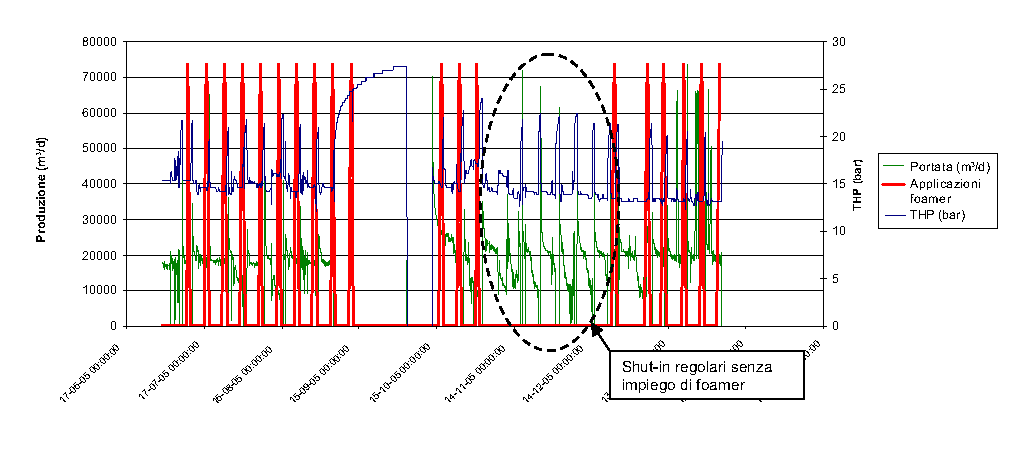
\includegraphics[width=\textwidth]{fig/foamer/batch-cycle.eps}
    \caption{Applicazione di \textit{foamer} in-batch su un pozzo con produzione a shut-in programmati \parencite{wittfeld2015foam}.}
    \label{fig:bacth-cycle}
\end{figure}

In rosso sono indicati i batch di schiuma applicati in pozzo. L'applicazione è stata poi fermata per 6-7 settimane per verificare l'efficacia dell'impiego di tensioattivi per il sollevamento artificiale dell'acqua. L'applicazione permette di avere produzioni molto più costanti, infatti i valori di portata tra uno \textit{shut-in} e l'altro sono pressoché identici. \textcite{wittfeld2015foam} ha confermato l'efficacia dell'applicazione trattando circa 60 pozzi. Trascurando i pozzi in cui non è stato possibile applicare il \textit{foamer}, nel 50\% dei casi si sono avuti degli evidenti miglioramenti di performance, il 30\% non presenta elementi sufficienti per affermare o negare l'utilità del metodo, nel 20\% la produzione di gas non risente affatto dell'applicazione.\\
L'impiego di schiumogeni in-batch richiede condizioni specifiche per garantire una buona riuscita dell'applicazione:
\begin{itemize}
    \item \textbf{rapporto acqua-condensati (\textit{Water to Condensate Ratio}, WCR)}: gli idrocarburi condensati agiscono come antischiuma naturali e diminuiscono le performance dello schiumogeno;
    \item \textbf{tipi di condensato}: condensati di idrocarburi pesanti diminuiscono le performance della schiuma in maniera più decisa rispetto a condensati di idrocarburi leggeri;
    \item \textbf{impiego di altri prodotti chimici}: alcuni additivi chimici, come per esempio degli agenti anticorrosivi, sono conosciuti propriamente anche come \textit{defoamer};
    \item \textbf{solidi in sospensione o disciolti}: la formazione di schiuma risente della presenza di solidi nella soluzione liquida, sia sospesi (e.g. \ce{Fe S}) che disciolti (e.g. sali).
\end{itemize}

I costi di tale applicazione si aggirano a €xxx per batch e variano a seconda di quanti pozzi possono essere raggiunti in giornata: si tende quindi a trattare più pozzi nella stessa giornata al fine di spalmare i costi fissi della manodopera e della strumentazione in affitto.

\subsection{Schiumogeni in continuo}
L'applicazione di schiumogeno in continuo avviene tramite l'installazione di una \textit{capillary string} attraverso la croce di produzione, all'interno del tubino di produzione per scendere fino all'altezza desiderata di iniezione del \textit{foamer}. La \textit{capillary string} può essere installata anche in presenza di una valvola di sicurezza di fondo  (\textit{Surface Controlled Subsurface Safety Valve}, SCSSV), previa modifica di quest'ultima.

\begin{figure}[htbp]
    \centering
    \includegraphics[width=\textwidth]{fig/foamer/continuous.eps}
    \caption{Schema generale di sistema di iniezione \textit{foamer} in continuo tramite \textit{capillary string} \parencite{wittfeld2015foam}.}
    \label{fig:continuous}
\end{figure}

I nuovi dispositivi di controllo idraulico in superficie devono rimanere indipendenti rispetto a quelli già esistenti sul campo, visto che il loro funzionamento avviene rispettivamente tramite tensioattivi liquidi e olio idraulico. Ciò comporta anche alla sostituzione di parte del sistema già esistente. La scelta obbligata della sostituzione è dettata dal fatto che lo schiumogeno non deve mai entrare in contatto con l'olio idraulico per questioni di sicurezza, soprattutto durante fasi delicate come l'attivazione del sistema di chiusura d'emergenza (o \textit{Emergency ShutDown}, ESD). La strumentazione superficiale di controllo iniezione, mostrata in \figref{fig:continuous}, prevede:
\begin{itemize}
    \item[(1)] \textbf{contenitore IBC (\textit{Intermediate Bulk Container})}: tipicamente il \textit{foamer} è distribuito e conservato in \textit{bulk} costituiti da una gabbia tubolare in acciaio zincato assicurata ad un pallet dalla capacità di 1000 litri. Sul campo al contenitore IBC viene associato un contenitore più piccolo a monte, in modo da garantire la continuità dello schiumogeno in caso di sostituzione del \textit{bulk} principale. Si preferisce utilizzare pallet trasparenti così da garantire all'operatore il controllo visivo del livello di \textit{foamer};
    \item[(2)] \textbf{filtro}: filtro meccanico con maglie da \SI{20}{\um} a protezione dei dispositivi a valle da eventuali impurità;
    \item[(3)] \textbf{pompa}: solitamente a pistone, le pompe di iniezione lavorano a una pressione massima di 400 bar, rapporto di \textit{turndown} di 10:1 circa e capacità massima di crica 100 litri al giorno;
    \item[(4)] \textbf{valvola di rilascio in pressione (\textit{Pressure Safety Valve}, PSV)}: configurata sulla base dell'equipaggiamento sotterraneo, solitamente a \SI{300}{bar} circa;
    \item[(5)] \textbf{sistemi di misura}: un misuratore di portata massica associato a un misuratore di pressione per il monitoraggio continuo del sistema;
    \item[(6)] \textbf{valvola a tre vie}: collocata a valle della pompa, è fondamentale per l'intero sistema ESD, in caso di chiusura della SCSSV la valvola a tre vie devia il flusso a un contenitore libero o a un separatore.
\end{itemize}

La strumentazione in sotterraneo, sempre visibile in \figref{fig:continuous} comprende:
\begin{itemize}
    \item[(7-10)] \textbf{SCSSV modificata}: come già detto la \textit{capillary string} può lavorare anche in presenza della valvola di sicurezza di fondo, la quale richiede però una modifica affinché questo sia possibile. Il \textit{foamer} passa dalla linea di controllo idraulico (\textit{control line}) e dentro il foro sigillato del raccordo di alloggiamento (\textit{landing nipple}). Da qui lo schiumogeno può pressurizzare il \textit{flapper} (o la sfera) della SCSSV in modo da aprirlo, oppure può scorrere lungo la parete esterna della valvola grazie alla \textit{capillary string}, per poi essere iniettato tramite la valvola LK-2;
    \item[(11)] \textbf{valvola di iniezione LK-2}: regola l'iniezione del \textit{foamer} e si trova direttamente al di sotto della valvola di fondo. Una configurazione ideale prevede una pressione di apertura della SCSSV a 70 bar e una pressione di apertura della LK-2 a 150 bar, in modo da consentire di mantenere aperta la valvola di fondo senza iniezione di schiumogeno.
    \item[(12)] \textit{\textbf{capillary string}}: solitamente è impiegata una \textit{capillary string} da {\sfrac{1}{4}}" OD (\textit{Outside Diameter}, diametro esterno) con uno spessore della parete di 0,035". Il materiale è solitamente Incoloy 625, una lega a base di nickel eccellente in ambienti corrosivi e dalle alte temperature. La capillary string può essere applicata fino a una profondità di 4000 m, dopo la quale l'intero sistema può collassare sotto l'azione del peso proprio.
    \item[(13)] \textbf{doppia valvola di contropressione}: doppia barriera a sicurezza del pozzo durante l'installazione del sistema, tipicamente configurata per tenere la testa idrostatica della \textit{capillary string}, dove però la regolazione è sempre a opera della LK-2.
\end{itemize}
Il controllo della schiuma avviene a opera di sistemi indipendenti di pompaggio antischiuma, simile a quello impiegato per il \textit{foamer} ma che differisce per alcuni aspetti:
\begin{itemize}
    \item assenza della valvola a tre vie;
    \item nessuna valvola di controllo di alta e bassa pressione (\textit{Pressure Control Valve}, PCV);
    \item capacità di iniezione massima di \SI{15}{\litre\per\hour}.
\end{itemize}
\textcite{wittfeld2015foam} ha testato gli schiumogeni in continuo su 7 pozzi, 4 dei quali hanno risposto ottimamente all'applicazione. La \figref{fig:continuous-evaluation} mostra l'andamento di un pozzo trattato con successo tramite iniezione in continuo di \textit{foamer}. 
\begin{figure}[htbp]
    \centering
    \includegraphics[width=\textwidth]{fig/foamer/continuous-evaluation.eps}
    \caption{Valutazione pre- e post-applicazione di \textit{foamer} in continuo su un pozzo affetto da \textit{liquid loading} \parencite{wittfeld2015foam}.}
    \label{fig:continuous-evaluation}
\end{figure}
Il pozzo era caratterizzato da produzione incostante e veniva aperto solo per brevi periodi. Una volta iniziata l'applicazione di schiumogeno in continuo, la produzione di gas si è notevolmente stabilizzata, con portate medie quasi raddoppiate. Il pozzo ha mantenuto questo andamento e ha garantito produzione di gas per 9 mesi.\\
Alcune sono le condizioni affinché l'applicazione abbia esiti positivi:
\begin{itemize}
    \item \textbf{risposta positiva al \textit{foamer} in-batch}: se un pozzo risponde bene alle applicazioni in-batch, esso può considerarsi un ottimo candidato all'applicazione di schiumogeno in continuo. Questa condizione risulta essere importante ma non necessaria: se un pozzo non reagisce in maniera positiva ai batch di schiuma, non vuol dire in modo assoluto che non sia un candidato idoneo per l'iniezione tramite \textit{capillary string};
    \item \textbf{riduzione sufficiente della portata critica}:  una volta applicato il \textit{foamer} in continuo, il pozzo deve comunque avere sufficiente energia per spiazzare l'acqua e evitare nuovamente l'aumento del battente idrostatico a fondo pozzo. Come già detto all'inizio del paragrafo ~\ref{section:foamer-ll} l'applicazione di \textit{foamer} porta a riduzioni della portata critica fino al 33\%, ciò vuol dire che il pozzo deve avere energia sufficiente a garantire il 66\% della portata critica standard;
    \item \textbf{ottimizzazione del IPR}: è utile stimare le variazioni di IPR dopo l'applicazione del schiumogeno in modo da verificare l'entità della variazione dello stesso parametro. Se la variazione risulta eccessiva, l'installazione della \textit{capillary string} non è particolarmente consigliata;
    \item \textbf{accesso al pozzo}: è necessario che il pozzo non presenti ostacoli o particolari restringimenti per l'installazione della \textit{capillary string} fino alla profondità desiderata;
    \item \textbf{disponibilità a test temporanei}: in alcuni casi, è opportuno condurre un test di 4-5 giorni per verificare l'efficacia del test, il pozzo deve essere quindi predisposto all'installazione anche solo temporanea del sistema di iniezione.
\end{itemize}
I costi legati all'impiego di un sistema di iniezione in continuo sono legati agli investimenti iniziali e ai costi in vita. L'investimento iniziale prevede le modifiche della strumentazione di superficie (~€xxx), l'acquisto della \textit{capillary string} (~€x per metro), la modifica all'SCSSV (~€xxx) e l'installazione della strumentazione in sotterraneo (personale di terra già presente), per una spesa totale di ~€xxxx. I costi in corso di utilizzo sono legati all'impiego di \textit{foamer} e \textit{defoamer} (~€x per litro, quindi ~€xxxx all'anno) e i costi di manutenzione e riparazione (~€xxx), per un totale di ~€xxxx di spese medie annuali.  \\ \\
L'intero impianto di produzione e trattamento del gas risente notevolmente dei miglioramenti di performance del pozzo: una produzione più regolare consente di trattare il gas in modo più idoneo e sicuro, senza dimenticare che l'aumento di portata garantisce maggiori introiti giornalieri. Per conoscere i vantaggi anche a livello impiantistico, nel prossimo capitolo viene fornito un \textit{excursus} sull'estrazione del gas e i successivi trattamenti subiti prima dell'immissione nella rete nazionale.
\clearpage{\pagestyle{empty}\cleardoublepage}
\chapter{Impianti di trattamento del gas naturale}\thispagestyle{empty}
\chaptermark{Trattamento gas naturale}
Per trattamento di gas naturale si intende l'insieme delle operazioni utili alla riduzione o abbattimento dei componenti che possono incidere sul trasporto e sull'utilizzo ultimo della risorsa. Le reti di distribuzione su larga scala prevedono delle specifiche tecniche e i trattamenti sono mirati al fine di ottenere valori che rispettino questi criteri. La produzione di gas naturale è normalmente associata alla presenza di acqua, la quale può presentarsi in forma liquida o gassosa. Il trattamento della disidratazione è fondamentale al fine di impedire la formazione di idrati, composti solidi che possono danneggiare le condotte durante il trasporto. Altri trattamenti sono legati al recupero degli idrocarburi condensati, che si manifestano al cambiare delle condizione di pressione e temperatura in superficie, e alla presenza di elementi corrosivi e elementi inerti, che possono diminuire i rendimenti del gas naturale.
Il trattamento definitivo del gas può essere preceduto da un trattamento provvisorio (\figref{fig:generaltreatment}), nel quale si riducono o si inibiscono momentaneamente gli effetti dei componenti indesiderati del gas. Solitamente si fa riferimento al trattamento provvisorio nel trasporto del gas prodotto dall'area pozzo alla centrale di trattamento.

\begin{figure}[htbp]
    \centering
    \includegraphics[width=\textwidth]{fig/impianti/generaltreatment.eps}
    \caption{Tipologie di trattamento.}
    \label{fig:generaltreatment}
\end{figure}

Nel seguente capitolo si espongono le specifiche tecniche del gas, i processi di trattamento e le relative apparecchiature e impianti.

\section{Specifiche del gas di vendita}
Il gas naturale è una miscela di idrocarburi solitamente allo stato gassoso costituita in gran parte da metano e da idrocarburi più pesanti. Altre componenti spesso presenti sono acqua, anidride carbonica, azoto, idrogeno solforato e solfati, in alcuni casi anche elio e metalli pesanti come mercurio. In \tabref{tab:ng-composition} è riportato un esempio di composizione centesimale di un gas naturale. 

\begin{table}[htbp]
    \small
    \centering
    \caption{Composizione centesimale di un gas naturale tramite cromatografia del gas \parencite{mele2012produzione}.}
    \label{tab:ng-composition}
    \begin{tabular}{p{.45\textwidth}p{.45\textwidth}}
        \hline
        {\bf Componenti}                & {\textbf{\% in volume}}       \\ \hline
        Azoto                           & {0,17}                        \\
        Anidride carbonica              & {0,02}                        \\
        Metano                          & {99,71}                       \\
        Idrogeno solforato              & {-}                           \\
        Etano                           & {0,06}                        \\
        Propano                         & {0,03}                        \\
        Iso-butano                      & {0,01}                        \\
        Neopentano                      & tracce                        \\
        Iso-pentano                     & -                             \\
        Esani                           & -                             \\
        Ottani                          & -                             \\
        Eptani                          & -                             \\ \hline
    \end{tabular}
\end{table}

Ai fini della distribuzione e vendita, il gas naturale deve rispettare parametri specifici per poter poi essere immesso nelle reti nazionali. La rete di distribuzione su larga scala non prevede alcun trattamento del gas, ma delle semplici compressioni e decompressioni a seconda delle esigenze dell'utente finale. Il gas deve essere quindi opportunamente trattato nel rispetto di tali specifiche.

\paragraph{Potere calorifico e indice di Wobbe}
Il gas naturale viene utilizzato maggiormente come combustibile e deve fornire un potere calorifico a specifica su tutto il territorio nazionale. Come parametro di riferimento si assume il potere calorifico superiore (PCS) pari a 9.100 kcal/Sm\ap{3} o 38,1 MJ/Sm\ap{3} (il PCS del gas metano puro è 9.001,6 kcal/Sm\ap{3}), con un campo di variabilità nell'ordine del ±10\%. \'E importante ricordare che il PCS di un gas naturale può raggiungere questi valori anche in presenza di gas inerti come anidride carbonica e azoto, essendo formato da idrocarburi superiori che innalzano notevolmente il potere calorifico medio.\\
A questo proposito è utile introdurre l'indice di Wobbe \(I_W\) definito come:
\[I_w = \dfrac{\textrm{PCS}}{\sqrt{\rho_s}} \label{eq:wobbe} \]
dove \(\rho_s\) è la densità specifica del gas (densità relativa rispetto a quella dell'aria). Se si prende come riferimento il metano, l'indice di Wobbe è pari a 12.094,8 kcal/Sm\ap{3} o 50.604,64 kJ/Sm\ap{3}, con una variabilità consentita del ±5\%. Nella valutazione della compatibilità di un gas per la sua immissione nella rete di distribuzione, è più corretto far riferimento all'indice di Wobbe: il campo di variazione più ristretto equivale a una minore presenza di gas inerti in miscela.

\paragraph{Punto di rugiada dell'acqua e degli idrocarburi}
Il gas non deve presentare condizioni di condensazione di acqua e/o idrocarburi in alcuna fase di trasporto e distribuzione. Le specifiche di pressione e temperatura variano a seconda delle diverse condizioni geografiche e climatiche, con queste anche i punti di rugiada (\textit{dew point}) dell'acqua e degli idrocarburi. Questi valori sono calcolabili tramite la rappresentazione del diagramma di fase relativo. Si considerano due specifiche diverse (in acqua e in idrocarburi) per i motivi seguenti:
\begin{itemize}
    \item \textbf{formazione di idrati}: si deve tenere maggiormente in considerazione la condensazione d'acqua rispetto a quella di idrocarburi a causa della formazione di idrati in condotta (trattati più avanti nel paragrafo ~\ref{section:dehidratation}). I margini operativi per la condensazione dell'acqua devono essere quindi più elevati;
    \item \textbf{andamento non univoco della saturazione rispetto alla pressione}: essendo il gas naturale una miscela multicomponente, nel definire la specifica di \textit{dew point} in idrocarburi non si fa riferimento, come in acqua, a una pressione prefissata, ma a tutto il campo i pressioni a partire da quella atmosferica. Il diagramma di fase di una miscela multifase, visibile in \figref{fig:phasediagram}, è caratterizzato dalla zona di condensazione retrograda: in questa condizione con una riduzione di pressione (a temperatura costante) gli idrocarburi condensano anziché evaporare.
\end{itemize}

\begin{figure}[htbp]
    \centering
    \includegraphics[width=.6\textwidth]{fig/impianti/phasediagram.eps}
    \caption{Diagramma di fase per una miscela multicomponente \parencite{bianco2005impiantigas}}
    \label{fig:phasediagram}
\end{figure}

\paragraph{Gas inerti (\ce{CO2} e \ce{N2})}
L'anidride carbonica (\ce{C O2}) in giacimento nasce dall'iterazione delle acque di strato con i silicati e i carbonati presenti. Raramente l'acido carbonico, composto che si forma per idratazione dell'anidride carbonica: 
\[\ce{H2O + CO2 -> H2CO3} \addtag \label{eq:acidocarbonico}\]
rappresenta un problema concreto per gli impianti di trasporto del gas naturale. Il contenuto di \ce{CO2} nel gas naturale non influenza significativamente l'indice di Wobbe, ma contribuisce all'incremento dei gas inerti totali (l'azoto \ce{N2} e appunto l'anidride carbonica). Si preferisce comunque rimuovere il \ce{CO2} (fino al raggiungimento dell'indice di Wobbe) rispetto all'azoto per la sua facilità tecnica di abbattimento. In generale si parla di volumi accettabili di \ce{CO2} attorno al 3\% con un contenuto totale di gas inerti che non deve mai superare il 6,5\%.

\paragraph{Acido solfidrico (\ce{H2S})}
L'acido solfidrico o idrogeno solforato (\ce{H2S}) è un gas incolore dall'odore caratteristico di uova in decomposizione. \'E presente naturalmente nel petrolio e nel gas naturale e rappresenta uno dei sottoprodotti della decomposizione di proteine contenenti zolfo e dalla riduzione diretta di solfati (\ce{SO4^2-}) da parte di batteri, funghi e attinomiceti presenti in ambiente anossico. L'\ce{H2S} è la principale causa di corrosione nella produzione di gas naturale, è altamente tossico e, per certe concentrazioni, anche mortale. Il contenuto massimo accettato è molto basso: Snam Rete Gas richiede un contenuto massimo di 6,6 mg/Sm\ap{3}.

\paragraph{Zolfo totale}
L'abbattimento dello zolfo totale nel gas naturale è legato più a questioni ambientali che a questioni di sicurezza. Il contenuto di zolfo totale massimo richiesto da Snam Rete Gas è di 150 mg/Sm\ap{3}, con un valore massimo di zolfo da mercaptani 15,5 mg/Sm\ap{3}. La rimozione dei mercaptani avviene tramite impianti che differiscono da quelli utilizzati per la rimozione di acido solfidrico e altri acidi.

\paragraph{Solidi sospesi}
I solidi sospesi vengono normalmente abbattuti durante i processi di separazione dei liquidi dal gas. Solo in casi particolari il gas naturale viene posto a processi di filtrazione meccanica.

\begin{table}[htbp]
    \small
    \centering
    \caption{Parametri di controllo della qualità richiesti dalla Snam Rete Gas \parencite{snam2015codice}.}
    \label{tab:ng-specifiche}
    \begin{tabular}{p{.4\textwidth}p{.2\textwidth}p{.23\textwidth}}
        \hline 
        {\bf Parametri} & \multicolumn{1}{l}{{\bf Valori consentiti}} & {\bf Unità di misura} \\ \hline \hline
        Potere Calorifico Superiore & 34,95 ÷45,28 & MJ/Sm\ap{3} \\\hline
        Indice di Wobbe & 47,31÷52.33 & MJ/Sm\ap{3} \\\hline
        Densità relativa & 0.5548÷0,8 &  \\\hline
        Ossigeno & \(\leq\) 0,6 & \% mol \\\hline
        Punto di Rugiada dell'acqua (p=7 MPa) & \(\leq\) -5 & °C \\\hline
        Punto di Rugiada degli idrocarburi (p=0,1÷7 MPa) & \(\leq\) 0 & °C \\\hline
        Temperatura max & \textless 50 & °C \\\hline
        Solfuro di idrogeno & \(\leq\) 6,6 & mg/Sm\ap{3} \\\hline
        Zolfo da mercaptani & \(\leq\) 15,5 & mg/Sm\ap{3} \\\hline
        Zolfo Totale & \(\leq\) 150 & mg/Sm\ap{3} \\ \hline
    \end{tabular}
\end{table}

\section{Separazione gas-liquido}
La dinamica delle particelle disperse in un fluido studia i fenomeni di sedimentazione di gocce di liquido in un gas applicando gli stessi principi della separazione per gravità liquido-liquido. Il calcolo della velocità terminale \(w_t\) viene effettuato in base al bilancio statico delle forze che agiscono sulla singola particella, condizione nella quale la velocità è costante. Nel caso di particelle sferiche indeformabili di raggio \(D_p\)
\[w_t=\sqrt{\dfrac{4 \; g \; D_p(\rho_p-\rho_f)}{3 \; C_D \; \rho_l}} \addtag \label{eq:velterminale}\]
dove \(g\) è l'accelerazione di gravita, \(\rho_p\) e \(\rho_f\) sono la densità rispettivamente della particella e del fluido disperdente, \(C_D\) è definito coefficiente di galleggiamento o \textit{drag coefficient}. Nel caso di separazione per gravità liquido-liquido e condizioni di moto laminare, quindi per bassi valori del numero di Reynolds \(R_e\), la \eqref{eq:velterminale} assume la forma della legge di Stoke:
\[w_t= \dfrac{(\rho_p-\rho_f)}{18\mu} \; D_p^2\; g \addtag \label{eq:stoke}\]
Per quanto riguarda particelle fluide immerse in un gas la condizione di moto laminare non è rispettata, a causa dei bassi valori della viscosità del gas quindi dell'alto valore del numero di Reynolds. In questo caso il calcolo del coefficiente di galleggiamento è effettuato tramite modelli sperimentali e calcolo per tentativi (\textit{trial and error}). La separazione per gravità è un processo grossolano che permette l'abbattimento di particelle nell'ordine di \SI{250}{\um} o di poco inferiore. Gli abbattitori (anche \textit{knockout} o KOD, \textit{Knock-Down Drum}) sono particolari separatori che agiscono per semplice gravità, utili per eliminare o solo l'acqua liquida o tutto il fluido trascinato dal gas. Sono generalmente collocati a monte di impianti di separazione meccanica a bassa temperatura (par. ~\ref{subsection:lts}) o a protezione di una fiaccola. Il dimensionamento dei KOD è basato sul bilancio tra tempo di ritenzione e tempo di decantazione delle particelle liquide in flusso gassoso.
Nei casi in cui si vogliano ottenere delle migliori performance di abbattimento dei liquidi si deve ricorrere a unità snebbianti che facilitino la coalescenza delle gocce e favoriscano l'abbattimento di gocce con diametro superiore ai \SI{10}{um}. Una delle unità snebbianti più comunemente utilizzate è il pacco rete (\textit{wire mesh pad}), inserito perpendicolarmente al flusso del gas. L'equazione che determina la velocità massima nella materassina snebbiante (\textit{mist eliminator}) è:
\[ w_t=K \sqrt{\dfrac{\rho_p-\rho_f}{\rho_f}} \addtag \label{eq:rete}\]
dove costante K varia in base al separatore e alla pressione operativa.\\
Nel campo della separazione di liquidi dal gas sono molto utilizzati anche i cicloni e i pacchi vani. I cicloni sono unità di coalescenza che sfruttano l'effetto centrifugo ottenuto tramite il movimento circolare del gas, con abbattimento delle particelle liquide fino ai \SI{3}{mu}. I pacchi di vani sono elementi coalescenti molto utilizzati anche nel trattamento dell'olio e sfruttano l'"effetto chicane" che si instaura nel flusso. Queste due unità di coalescenza sono preferite per il trattamento di gas caratterizzato da un notevole contenuto di solidi, come cristalli di paraffina separatisi dalla fase liquido in condizioni di bassa temperatura.

\section{Disidratazione e degasolinaggio} \label{section:dehidratation}
La variazione delle condizioni operative può dar luogo a fenomeni di condensazione di idrocarburi e/o acqua a partire da una miscela di idrocarburi allo stato gassoso. Quando in una corrente di gas naturale si ha la formazione di acqua libera, per determinate condizioni di flusso possono formarsi dei composti solidi detti idrati.
Il termine "idrato" è un termine generico per intendere nello specifico i composti di inclusione o clatrati (dal latino \textit{clauthratus}, ingabbiato), strutture molecolari in cui un tipo di molecole avvolge un altro tipo di molecole. Le prime sono dette molecole ospitanti mentre le altre molecole ospiti. Per gli idrati di gas naturale le molecole ospitanti sono le molecole di acqua, mentre le molecole ospiti sono le molecole costituenti il gas naturale. La particolare conformazione è stabile in fase solida, dove le molecole ospitanti formano un reticolo cristallino al cui interno si generano della cavità in cui si posizionano le molecole di gas. 
A differenza del ghiaccio, la formazione degli idrati è fortemente dipendente dalle condizioni di pressione: maggiore è la pressione parziale del gas (quindi la concentrazione di molecole ospiti), maggiore è la temperatura di formazione degli idrati. La tendenza a formare idrati negli idrocarburi leggeri aumenta con il peso molecolare dell'idrocarburo e la presenza di anidride carbonica (\ce{CO2}) e solfuro di idrogeno (\ce{H2S}). 
In generale, affinché gli idrati si possano formare è necessario che si instaurino le seguenti condizioni:
\begin{itemize}
    \item presenza acqua allo stato liquido;
    \item presenza di idrocarburi;
    \item moto turbolento;
    \item pressione e temperatura.
\end{itemize}
Sono stati sviluppati dei diagrammi che consentono di prevedere la formazione di idrati a determinate condizioni di pressione e temperatura, in funzione alla densità o peso molecolare medio del gas \figref{fig:formazioneidrati}.
\begin{figure}[htbp]
    \centering
    \includegraphics[width=.5\textwidth]{fig/impianti/formazioneidrati.eps}
    \caption{Diagramma della formazione degli idrati in funzione di temperatura e pressione \parencite{bianco2005impiantigas}.}
    \label{fig:formazioneidrati}
\end{figure}
Gli idrati possono formarsi all'interno delle singole condotte o concentrate su un collettore e possono danneggiare l'impianto in numerosi modi. L'occlusione parziale o totale della condotta porta a un aumento incontrollato della pressione a monte del tappo di idrati con conseguente rottura della linea o per squarciamento della stessa o per impatto in corrispondenza di una curva (\figref{fig:idrati1}). Il tappo di idrati soggetto a riscaldamento localizzato può espandersi in modo incontrollato, portando all'inevitabile rottura della condotta (\figref{fig:idrati2}). Con l'interruzione di produzione a opera di una valvola, se la velocità del tappo è sufficientemente elevata, la quantità di moto degli idrati può produrre pressioni così elevate da far scoppiare la linea (\figref{fig:idrati3}).

\begin{figure}[htbp]
    \centering
    \subfloat[][Rottura per impatto di idrati su elemento curvo della condotta.]
    {\includegraphics[width=.45\textwidth]{fig/impianti/idrati/idrati2.eps}  \label{fig:idrati1}} \qquad
    \subfloat[][Rottura per riscaldamento e espansione incontrollata.]
    {\includegraphics[width=.45\textwidth]{fig/impianti/idrati/idrati1.eps} \label{fig:idrati2}} \\
    \subfloat[][Rottura per inerzia del tappo di idrati.]
    {\includegraphics[width=.45\textwidth]{fig/impianti/idrati/idrati3.eps} \label{fig:idrati3}} 
\caption{Danni in condotta creati dalla formazione di idrati \parencite{borghi2005idrati}.}
\label{fig:idrati}
\end{figure}

Si inibisce la formazione di idrati in via temporanea aumentando la temperatura di trasporto del gas o tramite l'impiego di inibitori chimici, in via del tutto definitiva con la completa disidratazione chimica.

\subsection{Inibizione chimica}
Gli inibitori vengono utilizzati per brevi tratti di linea, come i collegamenti tra le aree pozzo e le centrali di trattamento del gas naturale. Gli inibitori di idrati sono composti ad alta igroscopicità e possono agire in fase sia gassosa che liquida come l'alcol metilico (\ce{CH3-OH}), sia in fase solo liquida come il glicol monoetilenico o EG(\ce{C2H6O2}) e dietilenico o DEG(\ce{C4H10O3}). Il glicol è preferito all'alcol metilenico per la minore volatilità e infiammabilità.
Gli inibitori agiscono sul flusso gassoso in modo da abbassare il punto di congelamento spostando la formazione degli idrati verso valori più bassi di temperatura. La quantità o la concentrazione di glicol da iniettare è legata alle condizioni operative con cui si intende trasportare il gas naturale. La \figref{fig:inibizioneidrati} mostra l'abbassamento della temperature relativa alla curva di formazione degli idrati in funzione della concentrazione di EG (glicol etilenico o etilenglicol) disciolto in acqua.

\begin{figure}[htbp]
    \centering
    \includegraphics[width=.5\textwidth]{fig/impianti/inibizioneidrati.eps}
    \caption{Inibizione degli idrati tramite glicol etilenico \parencite{bianco2005impiantigas}.}
    \label{fig:inibizioneidrati}
\end{figure}

La rigenerazione del glicol, diluito in acqua all'arrivo della condotta, avviene tramite ebollizione dell'acqua in condensa, solitamente alla temperatura di 130°C.
Mentre in passato l'inibizione degli idrati era un sistema impiegato spesso per il trasporto del gas naturale dalle aree pozzo alla centrale di trattamento, oggi si preferisce installare un sistema di disidratazione in prossimità del sito di produzione, soprattutto quando le condotte sono di notevole lunghezza.

\subsection{Disidratazione per raffreddamento} \label{subsection:lts}
Uno dei sistemi più semplici per la disidratazione di un gas consiste nel raffreddamento del gas stesso. La temperatura finale del trattamento deve coincidere con il punto di rugiada che si vuole ottenere. La disidratazione per raffreddamento, condizionamento a freddo o separazione a bassa temperatura (\textit{Low-Temperature Separation}, LTS) si ottiene sfruttando l'effetto Joule-Thomson: grazie alla semplice espansione, la corrente gassosa riesce a diminuire la propria temperatura senza l'ausilio di energia esterna. L'intero processo viene ottimizzato tramite uno scambio termico carica-effluente a opera di uno scambiatore gas-gas, tale da sfruttare le temperature raggiunte nel processo come punti di pre- e post-trattamento del gas naturale. Gli impianti LTS richiedono pozzi a gas ad alta pressione che garantiscano un sufficiente salto entalpico. Le basse temperature permettono di ottenere un sensibile abbassamento del punto di rugiada del gas e un maggiore recupero di condensato rispetto ai separatori tradizionali. \\
Gli impianti di separazione a bassa temperatura (\figref{fig:lts}) si basano su due elementi di processo fondamentali:
\begin{itemize}
    \item separatore a bassa temperatura;
    \item scambiatore di calore.
\end{itemize}

\begin{figure}[htbp]
    \centering
    \includegraphics[width=.7\textwidth]{fig/impianti/lts.eps}
    \caption{Condizionamento del gas tramite separatore a bassa temperatura \parencite{bianco2005impiantigas}.}
    \label{fig:lts}
\end{figure}

Il separatore a bassa temperatura, anche detto separatore a freddo o a espansione, rappresenta il fulcro dell'impianto. Il gas viene immesso nella parte superiore del separatore tramite una duse. L'espansione del gas provocato dalla duse porta a una diminuzione repentina della temperatura del flusso con la condensazione di acqua. L'acqua, precipitando verso il basso, forma degli idrati che si raccolgono anche essi nella sezione inferiore per gravità. I liquidi e gli idrati vengono raccolti e scaldati tramite il gas in arrivo dal pozzo tramite una serpentina immersa. Questo riscaldamento viene effettuato per abbattere gli idrati e far rievaporare nuovamente i componenti leggeri come metano e etano. Il rendimento del processo dipende fortemente dalla temperatura finale raggiunta, perciò si consiglia di isolare i separatori a bassa temperatura per aumentare le performance di separazione per condensazione.
Lo scambiatore di calore gas-gas svolge una duplice funzione: provvede al preraffreddamento del gas in ingresso all'impianto di condensazione e al riscaldamento del gas in uscita riducendo al minimo la formazione di idrati. \\
L'unità di separazione a freddo può essere dotata di iniezione di inibitori al fine di abbassare ulteriormente la possibilità che si possano creare degli idrati al proprio interno. L'iniezione avviene a valle dell'espansione del gas e il sistema viene munito di un'unità di rigenerazione del glicol associato all'acqua in uscita.\\
Se le pressioni di arrivo del gas non sono sufficienti affinché l'espansione raggiunga temperature desiderate, l'impianto può essere aiutato da un ciclo di refrigerazione esterno a freon o propano. In questo caso si parlerà di disidratazione per raffreddamento con refrigerante o CRC (\textit{Compression Refrigeration Cycle}) e la temperatura di separazione viene ottenuta con uno scambiatore (\textit{chiller}) in cui il fluido refrigerante evapora a bassa temperatura e sottrae calore al gas da trattare. Le altre componenti dell'unità di trattamento non differisco dall'impianto LTS fin qui descritto.\\
Gli impianti di separazione a freddo sono impiegati non solo per la disidratazione del gas ma anche per il recupero degli idrocarburi superiori e pesanti in fase gassosa. Per la trattazione specifica si rimanda al paragrafo ~\ref{subsection:gasolina}.


\subsection{Disidratazione mediante assorbimento con glicol}
In questo tipo di disidratazione la tipologia di glicol più utilizzata è il trietilenico o TEG (\ce{C6H14O4}), anche se in alcuni casi può essere impiegato il DEG o l'EG. Il TEG è preferito agli altri per la più alta temperatura di decomposizione, importante ai fini della rigenerazione del glicol. La \figref{fig:disidratazioneglicol} mostra uno schema semplificato di impianto per la disidratazione con glicol.
\begin{figure}[htbp]
    \centering
    \includegraphics[width=.7\textwidth]{fig/impianti/deidratazioneglicol.eps}
    \caption{Schema semplificato di disidratazione con glicol \parencite{bianco2005impiantigas}.}
    \label{fig:disidratazioneglicol}
\end{figure}
Una corrente di TEG concentrato viene iniettata nella parte superiore della colonna di disidratazione, al fondo della quale viene fatto confluire il gas naturale da trattare. Il contatto col gas del glicol, altamente igroscopico, con più stadi di equilibrio in controcorrente porta alla disidratazione della corrente gassosa in uscita alla testa della colonna di assorbimento. Il TEG umido, cioè diluito in acqua, giunge al fondo della colonna e viene raccolto e inviato all'impianto di rigenerazione. Il recupero avviene tramite distillazione della soluzione.
La colonna di rigenerazione è divisa in due parti dalla sezione di alimentazione del glicol, dove la parte superiore è definita di rettifica, quella inferiore di arricchimento. Il TEG condensato viene preriscaldato tramite serpentina installata all'interno della colonna di rigenerazione, che funge da condensatore per abbattere le perdite di TEG. \\
Prima dell'immissione il TEG ricco viene convogliato in una camera di flash o \textit{flash drum}, nel quale i gas associati vengono recuperati tramite espansione a bassa pressione alla testa del separatore. \\
Dopo un eventuale passaggio tramite filtri a maglia e a carboni attivi, Il TEG ricco giunge alla colonna di rigenerazione, riscaldata tramite ribollitore di fondo solitamente di tipo \textit{kettle}. La temperatura del bollitore varia in funzione del tipo di glicol utilizzato: nel caso di utilizzo di TEG la temperatura è leggermente superiore ai 200°C in quanto ai 207°C il TEG tende a degradare, con DEG e EG le temperature operative scendono in quanto degradano attorno ai 165°C.\\
Per il riscaldamento si possono utilizzare vari sistemi (come tubi di fiamma e tubi di fumo immessi nel bagno da scaldare, fascio tubiero tradizionale, riscaldatore elettrico a resistenze corazzate, olio caldo (\textit{hot oil}), l'installazione deve avere comunque un occhio di riguardo sulla distribuzione della temperatura, ovvero il riscaldamento deve essere uniforme su tutta la superficie della camera di rigenerazione. \\
Il TEG rigenerato cede gran parte del calore passando nello scambiatore carica-effluente, viene pompato alla pressione di assorbimento e raffreddato alla testa della colonna di assorbimento.\\
Il trattamento continuo di disidratazione per glicol risulta essere molto semplice e il sistema di rigenerazione permette di raggiungere degli ottimi valori di concentrazione finale di TEG (solitamente attorno  al 98\%). Se si vogliono ottenere concentrazioni maggiori, occorrono dei processi di rigenerazione spinta con le quali i valori sono prossimi al 99,98\%. I processi di rigenerazione spinta più comuni sono l'installazione di colonna di \textit{stripping} con gas (\textit{dryer}), la rigenerazione sottovuoto (pressioni prossime a 0,1 bar) o i sisemi Drizo (utilizzo di gas di \textit{stripping} ottenuto vaporizzando composti liquidi mediante un adeguato serpentino di riscaldamento).

\subsection{Disidratazione mediante adsorbimento con setacci molecolari}
Nel caso in cui si voglia avere una disidratazione pressoché totale si può disidratare la corrente gassosa tramite adsorbimento a letto solido. L'acqua e alcuni inquinanti polari come \ce{CO2}, \ce{H2S} e mercaptani sono adsorbiti da un zeoliti, cristalli altamente porosi appartenenti alla classe degli allumninosilicati. Essi hanno caratteristiche del tutto simili alle argille naturali: agiscono come un filtro molecolare (\textit{molecular sieve}), lasciando passare il gas e trattenendo le molecole polari. I cristalli di zeolite sono mischiati a dei leganti a base argillosa per ottenere i letti molecolari. L'adsorbimento è reversibile e i cristalli di zeolite possono essere rigenerati: le molecole adsorbite possono essere rilasciate in condizioni di alta temperatura o basse pressioni \parencite{grace2010techinf}. \\
Un tipico impianto di disidratazione è composto da due o più colonne di adsorbimento a setacci molecolari (solitamente tre, due in funzione e una in rigenerazione) e da un riscaldatore di gas di rigenerazione. L'adsorbimento di acqua si ottiene facendo confluire la corrente gassosa dall'alto verso il basso (\textit{down flow}) e il gas secco, in uscita dalla parte inferiore, viene immesso direttamente in rete. La rigenerazione dei setacci molecolari avviene tramite \textit{stripping}: il gas caldo di rigenerazione viene fatto fluire in senso opposto rispetto a quello di adsorbimento (\textit{up flow)}. L'aumento di temperatura consente la rimozione delle molecole polari adsorbite dai cristalli di zeolite e si associano alla corrente gassosa calda. Il gas di rigenerazione in uscita viene raffreddato e l'acqua viene separata per condensazione, mentre il gas viene riciclato verso i letti molecolari in funzione.\\
I setacci molecolari sono impiegati non solo per la disidratazione del gas ma anche per prodotti liquidi leggeri come GPL e condensati recuperati tramite LTS.

\begin{figure}[htbp]
    \centering
    \includegraphics[width=.7\textwidth]{fig/impianti/molecularsieve.eps}
    \caption{Schema di disidratazione a due letti \parencite{bianco2005impiantigas}.}
    \label{fig:molecularsieve}
\end{figure}

\subsection{Degasolinaggio} \label{subsection:gasolina}
Il degasolinaggio viene effettuato per rispettare le specifiche del punto di rugiada degli idrocarburi, utili a garantire degli standard di trasporto nella rete di distribuzione. Il condensato, anche definito gasolina, è un liquido che si ricava dalle frazioni meno volatili del gas come propano, butano, pentano e altri idrocarburi superiori (\tabref{tab:gasoline-composition}). La composizione della gasolina varia notevolmente a seconda della provenienza: gas associato a greggio, gas da giacimento a gas condensato, gas da giacimenti a gas. La gasolina si trova in fase gassosa alle condizioni di giacimento e in fase liquida alle condizioni di superficie. Il suo aspetto è quello di benzina o petrolio leggero, il colore può variare dal bianco paglierino, all'azzurro e rossastro.
\begin{table}[htbp]
    \small
    \centering
    \caption{Composizione centesimale stimata di gasolina da gas naturale tramite distillazione \parencite{anderson1924composition}.}
    \label{tab:gasoline-composition}
    \begin{tabular}{p{.70\textwidth}p{.20\textwidth}}
        \hline
        {\bf Componenti}                & {\textbf{\% in volume}}       \\ \hline
        Propano e butano                & {20}                          \\
        Isopentano                      & {13}                          \\
        N-pentano                       & {17}                          \\
        Isoesano                        & {9}                           \\
        N-esano                         & {15}                          \\
        Isoeptano                       & {8}                           \\
        N-eptano                        & {12}                          \\
        Ottani                          & {4}                           \\
        Olio assorbito                  & {2}                           \\ \hline
    \end{tabular}
\end{table}
Nel trattamento del gas proveniente da un giacimento di gas condensati il GOR (\textit{Gas Oil Ratio}) è molto alto e il gas associato è ricco di gas propano e butano e si realizza un terzo prodotto definito GPL, acronimo di gas di petrolio liquefatti (in inglese LPG, \textit{liquid petroleum gas}). Il GPL è una miscela di propano e butano con contenuti marginali di etano e di idrocarburi superiori e, in qualità di prodotto finito fruibile dall'utente finale, deve rispettare determinate specifiche tecniche. Lo stoccaggio del GPL per lunghi tempi (e.g. trasporto in mare) a pressione ambientale avviene tramite refrigerazione, per ridurre la volatilità e aumentare così la stabilità della miscela. Il processo più semplice e più impiegato per il degasolinaggio è basato sulla refrigerazione del gas. In particolare si fa riferimento alla separazione per raffreddamento per espansione (LTS) o per raffreddamento con refrigerante (CRC), impianti del tutto similari a quelli impiegati per la disidratazione.\\
Nell'unità di separazione a freddo il gas viene condensato mediate refrigerazione. Il processo è sempre bifase e la separazione acqua-idrocarburi (acqua eventualmente associata a glicol) avviene a valle tramite separatore bifase. In uscita dal separatore a freddo, l'acqua viene convogliata e trattata all'esterno mentre il condensato viene stabilizzato. La separazione gas-liquido a freddo in questo caso richiede sistemi di abbattimento delle goccioline più raffinati rispetto alla semplice materassina filtrante, poco indicata a causa della possibile formazione di cristalli di idrati e paraffina. L'impianto di separazione a freddo è indicato più per il trattamento dei condensati che per la semplice disidratazione poiché la variazione di fase degli idrocarburi, al contrario dell'acqua, risente delle condizioni di pressione.

\section{Altri trattamenti}
A seconda della composizione del gas di giacimento, il trattamento del gas naturale prevede ulteriori processi al fine di renderlo a specifica. \\
Il processo di addolcimento consiste nella rimozione dal gas naturale di gas acidi come \ce{CO2} e \ce{H2S} e consiste nell'assorbimento di tali sostanze mediante soluzioni alcaline. La reazione si basa quindi sulle reazioni di neutralizzazione tra acido debole e reagente basico. Requisito fondamentale del processo è la sua reversibilità. 
I reagenti più comunemente utilizzati sono le alcanolammine, ammine associate a gruppi alcanoli, gruppi alchilici o alcanoli a seconda che si tratti di un'ammina primaria, secondaria o terziaria. Le ammine accettano un protone sotto forma di ione idrogeno \ce{H+} tramite una reazione altamente esotermica. Trattandosi di fase liquida, il rendimento del processo di addolcimento dipende dalla velocità di reazione e dal passaggio della fase gassosa a quella liquida. La superficie di contatto tra le due fasi è proporzionale al rendimento di processo. La \figref{fig:ammine} mostra uno schema semplificato del trattamento di assorbimento con relativa rigenerazione delle alcanolammine. Il gas acido viene in contatto con la soluzione amminica e raffreddato nella colonna di assorbimento. Essendo la reazione altamente esotermica, le basse temperature favoriscono l'assorbimento. La soluzione al fondo della colonna viene convogliata in una camera di flash dove si separa parte del gas associato al liquido e la soluzione viene trasferita all'impianto di rigenerazione. Le alcanolammine sono rigenerate tramite stripping in corrente di vapore. Le ammine soffrono in modo particolare di degradazione termica, perciò la temperatura di rigenerazione è limitata e si preferisce l'utilizzo di soluzioni molto diluite.\\
\begin{figure}[htbp]
    \centering
    \includegraphics[width=.7\textwidth]{fig/impianti/ammine.eps}
    \caption{Lavaggio amminico \parencite{bianco2005impiantigas}.}
    \label{fig:ammine}
\end{figure}
L'addolcimento del gas può essere effettuato anche tramite soluzioni di carbonato potassico a caldo: al vantaggio del processo di assorbimento non esotermico (minor dispendio energetico dovuto al raffreddamento della colonna di assorbimento e minor esigenza di grandi superfici di scambio), si contrappone la necessità di reintegrare l'acqua che per alte temperature satura il gas trattato.\\
La rimozione parziale dei gas acidi al gas naturale si può ottenere tramite membrane semipermeabili: la corrente gassosa viene frazionata sulla base della permeabilità selettiva di alcuni composti polari rispetto agli idrocarburi.\\
Altri trattamenti che il gas naturale può subire sono il lavaggio del gas di coda, l'assorbimento fisico, la rimozione di \ce{H2S} tramite processi ossidativi, i filtri a carboni attivi.

\section{Apparecchiature di processo e impianti particolari}
I processi fin qui descritti possono realizzarsi tramite un impianto di trattamento, l'insieme delle infrastrutture utili a rendere il gas erogato dai giacimenti conforme ai requisiti di pressione, temperatura e qualità necessari all'immissione nella rete di distribuzione. L'impianto di trattamento è quindi progettato in base alle caratteristiche fisico-chimiche del gas naturale prodotto e alle specifiche di vendita. Nel seguente capitolo sono descritte le apparecchiature con le quali si realizzano i trattamenti richiesti.

\subsection{Separatori} %tesi+doc.ettore
I separatori sono gli apparecchi più utilizzati per la separazione di un flusso combinato liquido-gas dei suoi due componenti. I separatori sono classificati in base alla loro configurazione operativa:
\begin{itemize}
    \item \textbf{separatori orizzontali} (\figref{fig:corpo-singolo}): sono estremamente economici quando vengono trattati volumi importanti di gas. La disposizione orizzontale garantisce maggiori rendimenti rispetto a quella verticale per via del maggior tempo di permanenza delle goccioline nel separatore. Un separatore orizzontale a doppio corpo è definito \textit{slug-catcher} (\figref{fig:corpo-doppio}), con il corpo superiore completamente libero e il corpo inferiore che funge da polmone del liquido. La configurazione dello \textit{slug-catcher} permette di lavorare con alte portate e bruscamente variabili, a differenza del separatore singolo. I separatori a singolo o doppio corpo non sono particolarmente indicati per il trattamento di fluidi contenenti sabbia o fango, a causa della bassa capacità di eliminazione dei depositi e quindi l'accumulo degli stessi sul fondo;
    \item \textbf{separatori verticali} (\figref{fig:separatore-verticale}): nonostante le minori performance rispetto ai separatori orizzontali, sono comunque impiegati nell'ambito del trattamento del gas naturale quando i flussi sono caratterizzati da fango, sabbia o gas associato a olio. Inoltre, i separatori verticali sono preferiti in ambito off-shore, vista la scarsa disponibilità di spazio;
    \item \textbf{separatori sferici}: impiegati per la loro compattezza, i separatori sferici rappresentano un giusto compromesso tra i rendimenti di un separatore orizzontale e le ridotte dimensioni di ingombro del separatore verticale. Attualmente i separatori sferici sono poco impiegati in ambito tecnico-progettuale.
\end{itemize}
\begin{figure}[htbp]
    \centering
    \subfloat[][Separatore orizzontale a corpo singolo.]
    {\includegraphics[width=.45\textwidth]{fig/impianti/separatori/horizontal-separator.eps}  \label{fig:corpo-singolo}} \qquad
    \subfloat[][Separatore orizzontale a doppio corpo o \textit{slug-catcher}.]
    {\includegraphics[width=.45\textwidth]{fig/impianti/separatori/double-barrel.eps} \label{fig:corpo-doppio}} \\
    \subfloat[][Separatore verticale.]
    {\makebox[.6\textwidth]{\includegraphics[height=.45\textwidth]{fig/impianti/separatori/vertical-separator.eps}} \label{fig:separatore-verticale}} 
\caption{Separatori orizzontali e verticali bifase dotati di dispositivi snebbianti \parencite{peerless2009vane}.}
\label{fig:bifase}
\end{figure}
I separatori possono essere forniti di elementi interni come deflettori, dighe, materassina snebbiante e/o pacco lamellare (\figref{fig:pacco-lamellare}) nel caso in cui si voglia aumentare la performance di separazione per semplice gravità. A seconda della configurazione i separatori possono separare la fase liquida dalla fase gassosa oppure riescono a operare una separazione spinta: si parla in questo caso di separatori bifase o separatori trifase (\figref{fig:trifase-interno}).
\begin{figure}[htbp]
    \centering
    \subfloat[][Vista interna di un separatore trifase dotato di pacco lamellare e materassina snebbiante.]
    {\includegraphics[width=.55\textwidth]{fig/impianti/separatori/trifase.eps}  \label{fig:trifase-interno}} \qquad
    \subfloat[][Dettaglio del pacco lamellare.]
    {\includegraphics[width=.35\textwidth]{fig/impianti/separatori/pacco-lamellare.eps} \label{fig:pacco-lamellare}} 
\caption{Separatore trifase e del pacco lamellare \parencite{bianco2005impiantiolio}.}
\label{fig:trifase}
\end{figure}

\subsection{Scambiatori di calore}
Numerose sono le tipologie di scambiatori impiegati nell'industria del gas naturale. \\
I più semplici sono gli scambiatori a fasci tubieri e mantello (\textit{shell-and-tubes}, \figref{fig:tubieri}), dove il dispositivo viene attraversato dalle due correnti sul "lato mantello" e sul "lato tubi". Lo scambiatore a fasci tubieri garantisce ottime performance grazie all'estesa superficie di scambio di cui è dotato.

\begin{figure}[htbp]
    \centering
    \subfloat[][Sezione trasversale.]
    {\includegraphics[width=.6\textwidth]{fig/impianti/scambiatori/tubiero-a.eps}  \label{fig:tubieri-a}} \qquad
    \subfloat[][Direzione del flusso all'interno dello scambiatore.]
    {\includegraphics[width=.3\textwidth]{fig/impianti/scambiatori/tubiero-b.eps} \label{fig:tubieri-b}} 
\caption{Scambiatore di calore a fasci tubieri \parencite{guadagni2003prontuario}.}
\label{fig:tubieri}
\end{figure}

Altro dispositivo di scambio termico è lo scambiatore a piastre (\figref{fig:piastre}). Questa tipologia di scambiatore prevede un pacco di piastre rettangolari tutte uguali, ottenute da lamiera per stampaggio secondo diverse forme di corrugazione superficiale. I fluidi lambiscono le piastre attraverso canali che si formano tra esse. Le piastre sono sostenute da un telaio e tenute in pressione da quest'ultimo. Hanno il vantaggio di raggiungere coefficienti di scambio elevati e sono molto flessibili in caso di modifiche progettuali. Inoltre sono molto impiegati in campo off-shore grazie al poco spazio richiesto per l'installazione. Negli ultimi anni hanno preso piede i PCHE (\textit{Plate Compact Heat Exchanger}), un'evoluzione degli scambiatori a piastre, molto richiesti per via della loro ulteriore riduzione di ingombro.\\

\begin{figure}[htbp]
    \centering
    \subfloat[][Piastre dello scambiatore.]
    {\includegraphics[width=.45\textwidth]{fig/impianti/scambiatori/piatti-1.eps}  \label{fig:piatti-a}} \qquad
    \subfloat[][Ingresso e uscita dei due fluidi.]
    {\includegraphics[width=.45\textwidth]{fig/impianti/scambiatori/piatti-2.eps} \label{fig:piatti-b}} 
\caption{Scambiatore a piastre \parencite{guadagni2003prontuario}.}
\label{fig:piastre}
\end{figure}

\subsection{Compressori}
Il compressore è una macchina operatrice che opera su un fluido comprimibile con l'obiettivo di aumentarne la pressione. I compressori possono classificarsi in:
\begin{itemize}
    \item compressori volumetrici o a flusso intermittente;
    \item compressori dinamici o a flusso continuo.
\end{itemize}
 La scelta di un idoneo impianto di compressione si realizza tramite il calcolo del rapporto di compressione richiesto, cioè il rapporto tra la pressione di mandata e quello di aspirazione. Il raggiungimento della pressione finale può avvenire in un unico salto oppure tramite più processi in serie: si parla quindi rispettivamente di compressori monostadio o compressori multipli. In caso di compressione multistadio, il gas naturale viene raffreddato ad ogni step tramite refrigerazione interstadio fino alla temperatura di ingresso.
\paragraph{Compressori volumetrici}
I compressori volumetrici o a flusso intermittente sono macchine che riducono il volume del gas naturale per aumentare la pressione. I compressori volumetrici possono essere classificati a loro volta in alternativi e rotativi.\\
Nei compressori volumetrici alternativi (\figref{fig:compressori-1}) il processo di compressione è realizzato da un pistone che realizza una "corsa" all'interno di un cilindro dotato di valvole di aspirazione e mandata. In una prima fase il pistone porta a compressione il gas all'interno del cilindro che viene poi convogliato alla mandata. Quando il cilindro torna in posizione originale, la riduzione di pressione all'interno del cilindro porta all'apertura delle valvole di ingresso e al ritorno delle condizioni iniziali. Una volta chiuse le valvole di aspirazione il ciclo si ripete. I compressori alternativi sono utilizzati nella compressione di gas naturale per basse portate e alte pressioni e la loro alimentazione è a opera di turbine a gas accoppiate direttamente al compressore (hanno un numero di giri analogo). Gli svantaggi dei compressori alternativi sono legati ai costi di manutenzione non trascurabili e alla creazione di vibrazioni indesiderate e spinte orizzontali alternate. La \figref{fig:compressori-3} mostra un compressore alternativo a cilindri contrapposti, spesso usato in questo ambito.\\
I compressori volumetrici rotativi spostano e comprimono il gas naturale tramite l'azione di elementi in moto rotatorio. Nell'ambito del trattamento del gas naturale sono impiegati compressori volumetrici rotativi a vite (\textit{rotary screw}, \figref{fig:compressori-4}) costituiti da due rotori accoppiati, di forma elicoidale, che ruotano comprimendo e spostando allo stesso tempo il gas. L'efficienza della macchina dipende in gran parte dai giochi tra i due rotori. I compressori a vite sono utilizzati per gas a basse pressioni, permettono di raggiungere alti rapporti di compressione con un singolo stadio e il loro utilizzo è ormai consolidato negli impianti frigoriferi (e.g. compressione del \textit{flash gas}). 
\paragraph{Compressori dinamici}
I compressori dinamici sono macchine a flusso continuo in cui la compressione si realizza accelerando l'aria quando questa passa attraverso un un elemento rotante ad alta velocità. L'energia cinetica acquisita si trasforma in energia di pressione in parte nell'elemento rotante e in parte in un diffusore statico a valle della girante. I compressori dinamici possono essere centrifughi o assiali.\\
Nei compressori centrifughi (\figref{fig:compressori-5}) il gas viene accelerato in una girante e il flusso principale ha direzione radiale. Questi compressori possono essere monostadio o multistadio (\figref{fig:compressori-6}) e possono gestire portate di gas elevate con notevole flessibilità e mantenendo la pressione di mandata costante. I compressori centrifughi sono le macchine più diffuse nell'industria del gas naturale e hanno come unico limite la portata minima di aspirazione e la macchina motrice più utilizzata è il motore elettrico.\\
I compressori assiali provocano l'accelerazione del gas tramite un rotore palettato e il flusso principale acquisisce direzione assiale. Questi compressori sono impiegati soprattutto per la compressione dei fluidi frigoriferi abbinati alla liquefazione dello stesso.

\begin{figure}[htbp]
    \centering
    \subfloat[][Schema del compressore volumetrico alternativo.]
    {\includegraphics[width=.4\textwidth]{fig/impianti/compressori/compressori-1.eps}  \label{fig:compressori-1}} \quad
    \subfloat[][Schema di compressore rotativo a palette.]
    {\includegraphics[width=.4\textwidth]{fig/impianti/compressori/compressori-2.eps}  \label{fig:compressori-2}} \\ \qquad\subfloat[][Compressore alternativo a cilindri contrapposti.]
    {\includegraphics[width=.4\textwidth]{fig/impianti/compressori/compressori-3.eps}  \label{fig:compressori-3}} \quad \qquad\subfloat[][Compressore a vite.]
    {\includegraphics[width=.4\textwidth]{fig/impianti/compressori/compressori-4.eps}  \label{fig:compressori-4}} \\ \qquad\subfloat[][Compressore centrifugo monostadio.]
    {\includegraphics[width=.4\textwidth]{fig/impianti/compressori/compressori-5.eps}  \label{fig:compressori-5}} \quad \qquad\subfloat[][Compressore centrifugo multistadio di processo.]
    {\includegraphics[width=.4\textwidth]{fig/impianti/compressori/compressori-6.eps}  \label{fig:compressori-6}} 
\caption{Compressori \parencite{guadagni2003prontuario}.}
\label{fig:compressori}
\end{figure}

\subsection{Espansori}
Gli espansori più comunemente utilizzati in questo ambito sono le turbine a impulso radiale e le turbine assiali. Le turbine a impulsi radiali sono largamente utilizzate e solitamente queste macchine sono molto compatte. Hanno come unico svantaggio il rapporto di espansione limitato, al fine di mantenere un rendimento elevato. Le turbine assiali invece sono impiegate per potenze elevate e portate di gas rilevanti. L'impiego degli espansori non è oggi una prima scelta nel trattamento del gas naturale ma è un ottima alternativa nel campo della refrigerazione. Al contrario dei sistemi tradizionali (a effetto Joule-Thomson o refrigerazione meccanica), gli espansori sono macchine semplici e compatta e in alcuni casi non richiedono l'impiego di potenza esterna al ciclo.

\subsection{Impianti frigoriferi}
Molti processi di trattamento del gas si basano sulla refrigerazione. Il ciclo frigorifero tramite refrigerazione meccanica (\figref{fig:frigorifero}) si realizza tramite la condensazione di un fluido (solitamente freon) in pressione, il quale viene poi fatto espandere nell'evaporatore (\textit{chiller}) attraverso una valvola. All'uscita dall'evaporatore il fluido refrigerante riportato alla pressione originaria tramite un compressore per poi tornare in fase liquida tramite il condensatore. Il fluido refrigerante è scelto in base alla temperatura di evaporazione che si intende raggiungere. Spesso il ciclo frigorifero può svilupparsi in più stadi, nel caso in cui si vogliano raggiungere temperature molto basse.

\begin{figure}[htbp]
    \centering
    \includegraphics[width=.5\textwidth]{fig/impianti/frigorifero.eps}
    \caption{Refrigerazione meccanicao \parencite{bianco2005impiantigas}.}
    \label{fig:frigorifero}
\end{figure}

Come detto in precedenza, il trattamento provvisorio non prevede la totale rimozione dell'acqua dal gas naturale. Di conseguenza nel trasporto del gas naturale in centrale l'acqua può accumularsi negli avvallamenti della condotta, generando così una contropressione. Le cadute di pressione nel trasporto di un fluido in condotta non permettono di operare in modo adeguato e si cerca di diminuire il valore di contropressione tramite diverse soluzioni tecniche. In campo industriale vengono impiegati degli scovoli o \textit{pig}, dispositivi cilindrico o sferico per pulire, ispezionare e misurare le condotte. Nel prossimo capitolo saranno trattate le diverse tipologie di scovolo e le procedure di piggaggio di una condotta in pressione
\clearpage{\pagestyle{empty}\cleardoublepage}

\chapter{Sistemi di piggaggio di condotte in pressione}\thispagestyle{empty} 
\chaptermark{Piggaggio}
Il piggaggio, o anche detto \textit{pigging}, è un'applicazione nella quale un dispositivo cilindrico o sferico chiamato scovolo (o \textit{pig}), opportunamente dimensionato, viene spinto all'interno di una condotta tramite variazioni indotte di pressione e flusso del mezzo presente all'interno, tramite l'introduzione di un mezzo esterno o tramite movimento meccanico al fine di pulire, ispezionare, dosare inibitori chimici lungo la tubazione oppure per isolare delle sezioni specifiche della rete.\\
L'origine del termine inglese \textit{pig} è tuttora incerto: se da una parte viene proposto come l'acronimo di \textit{Pipeline Intervention Gadget}, dall'altra si fa riferimento al rumore che provoca lo scorrimento dello scovolo in condotta, simile al verso di un maiale \parencite{varghese2011intelligent}.\\
Durante gli anni '40 negli Stati Uniti il piggaggio aveva come fine principale la rimozione di paraffina per migliorare l'efficienza delle condotte a olio, quindi per aumentare la produzione e sopperire all'alta domanda legata alle attività belliche della Seconda Guerra Mondiale.\\
Nel mondo oggi il piggaggio è impiegato per numerosi scopi e la strumentazione  è progettata dagli ingegneri in base alle necessità legate all'applicazione.\\
Il seguente capitolo offre una panoramica riguardo al piggaggio delle condotte in pressione dove vengono mostrate le varie configurazioni degli scovoli, le finalità dell'applicazione, le procedure operative e la valutazione di soluzioni in caso di blocco del \textit{pig} in linea.

\section{Configurazione degli scovoli}
L'assemblaggio e configurazione dello scovolo di servizio prevede numerose soluzioni:
\begin{itemize}
	\item \textbf{a mandrino} (\figref{fig:mandrel}): gli elementi dello scovolo sono assemblati sul corpo centrale tramite numerosi bulloni;
	\item \textbf{a bullone singolo} (\figref{fig:singlebolt}): simile allo scovolo a mandrino, gli accessori dello scovolo in questo caso sono inseriti tramite un'unica bullonatura longitudinale;
	\item \textbf{a telaio fisso} (\figref{fig:solidcast}): sia le tenute che gli elementi guida solo tenuti assieme da un singolo componente in poliuretano;
	\item \textbf{a schiuma} (\figref{fig:foampig}): solitamente con struttura aperta di poliuretano, questi scovoli sono disponibili a diversa densità, a seconda dell'applicazione richiesta. Il rivestimento aumenta la resistenza a usura e la stabilità dell'utensile;
	\item \textbf{sfere} (\figref{fig:spherepig}): possono essere piene o riempite con aria, acqua o glicol, possono essere usate come tamponi o rimozione liquidi;
	\item \textbf{articolato} (\figref{fig:articulated}): composto da due o più scovoli uniti tra loro con sistemi di accoppiamento universale. Rappresenta la configurazione base degli scovoli intelligenti;

\end{itemize}

\begin{figure}[htbp]
    \centering
    \subfloat[][A mandrino.]
    {\includegraphics[height=.1\textheight]{fig/pig/configurazione/mandrel.eps}  \label{fig:mandrel}} \qquad
    \subfloat[][A bullone singolo.]
    {\includegraphics[height=.1\textheight]{fig/pig/configurazione/singlebolt.eps}  \label{fig:singlebolt}} \qquad 
    \subfloat[][A telaio fisso.]
    {\includegraphics[height=.1\textheight]{fig/pig/configurazione/solidcast.eps}  \label{fig:solidcast}} \\
    \subfloat[][A schuma.]
    {\includegraphics[height=.1\textheight]{fig/pig/configurazione/foam.eps}  \label{fig:foampig}} \qquad
    \subfloat[][Sfere.]
    {\includegraphics[height=.1\textheight]{fig/pig/configurazione/sphere.eps}  \label{fig:spherepig}} \\
    \subfloat[][Articolato.]
    {\includegraphics[height=.1\textheight]{fig/pig/configurazione/articulated.eps}  \label{fig:articulated}}
\caption{Configurazione dello scovolo \parencite{davidson2002introduction}.}
\label{fig:configurazione}
\end{figure}

Gli scovoli a mandrino e a bullone singolo si adattano alla richiesta specifica grazie all'installazione di diversi dispositivi sul corpo centrale:
\begin{itemize}
\item \textbf{spazzole} (\figref{fig:spazzole}):  impiegate in primo luogo per la rimozione di depositi compatti come calcare e prodotti da corrosione. Alcune spazzole sono specifiche per favorire l'azione degli inibitori di corrosione e dei biocidi in condotta;
\item \textbf{guarnizioni a tazza} (\figref{fig:tazze}): dispositivi di tenuta idraulica che consente lo spostamento unidirezionale dello scovolo attraverso la spinta di un fluido da monte. Sono utilizzati solitamente anche come dispositivi di \textit{batching};
\item \textbf{coppelle coniche} : molto simili alle guarnizioni a tazza, hanno una lieve variazione nella geometria della tenuta;
\item \textbf{dischi} (\figref{fig:dischi}): accessori utilizzati come tenute idrauliche, per la pulizia e come organi di supporto. A differenza delle guarnizioni a tazza e le coppelle coniche, uno scovolo dotato di dischi può muoversi in entrambe le direzioni;
\item \textbf{lame} (\figref{fig:lame}): tramite l'azione di taglio, provvedono alla rimozione di depositi morbidi come paraffina e fanghi, derivanti dal trasporto di olio in linea;
\item \textbf{magneti} (\figref{fig:magneti}): l'inserimento di potenti magneti sulla circonferenza permette allo scovolo non solo l'asportazione di materiale ferroso dalla condotta, ma anche di attivare i segnalatori posti all'esterno della condotta per monitorarne il tragitto;
\item \textbf{accessori per la misurazione}: possono essere di varia natura (calibri, dischi misuratori, dispositivi magnetici, etc.) e consentono l'ispezione interna della condotta.
%I singolo dispositivi possono essere accoppiati sullo stesso dispositivo, al fine di sopperire a più richieste con un unico passaggio dello scovolo in condotta (\figref{fig:assemblato}).
\end{itemize}

\begin{figure}[htbp]
    \centering
    \subfloat[][Scovolo con spazzole a molla.]
    {\includegraphics[height=.12\textheight]{fig/pig/tool/spazzolemolla}  \label{fig:spazzole}} \qquad
    \subfloat[][Scovolo con guarnizioni a tazza.]
    {\includegraphics[height=.12\textheight]{fig/pig/tool/tazze}  \label{fig:tazze}} \qquad
    \subfloat[][Scovolo con dischi.]
    {\includegraphics[height=.12\textheight]{fig/pig/tool/dischi}  \label{fig:dischi}} \\
    \subfloat[][Scovolo con lame di poliuretano.]
    {\includegraphics[height=.12\textheight]{fig/pig/tool/lame}  \label{fig:lame}} \qquad
    \subfloat[][Scovolo con magneti sulla circonferenza.]
    {\includegraphics[height=.12\textheight]{fig/pig/tool/magneti}  \label{fig:magneti}} \qquad
%    \subfloat[][Scovolo con spazzole circolari, guarnizioni a tazza e dischi.]
%    {\includegraphics[height=.12\textheight]{fig/pig/tool/assemblato}  \label{fig:assemblato}}
\caption{Componenti tipici di uno scovolo di servizio \parencite{williamson2015guide}.}
\label{fig:dispositivi}
\end{figure}

\section{Obiettivi del piggaggio}
Il piggaggio di una condotta viene oggi eseguito in tutte le fasi di vita di un impianto di processo. Data la sua versatilità, è di consuetudine per tutti i settori dell'industria di processo, perciò non esistono delle classificazioni universali degli scovoli impiegati. Una generica distinzione tra \textit{pig} può essere fatta in base all'operazione richiesta: si parla quindi di scovoli di servizio, scovoli per l'ispezione interna e scovoli gel.

\subsection{Scovoli di servizio}
Qui di seguito sono elencati i motivi legati generalmente all'impiego di scovoli di servizio:
\begin{itemize}
	\item \textbf{pulizia della condotta}: utile per migliorare le condizioni di flusso;
	\item \textbf{separazione dei fluidi} o \textit{\textbf{batching}}: scovoli di separazione tra diversi prodotti chimici da applicare in condotta;
%		\item \textbf{ispezione interna}: è importante monitorare le condizioni interne della condotta, così da prevedere eventuali rotture o imprevisti di produzione. Gli scovoli possono assumere numerose configurazioni (forma e dimensioni), obiettivo ultimo è il rilevamento di ammaccature, consumo interno della parete interna e crepe.
	\item \textbf{spiazzamento della condotta}: specialmente nelle condotte a gas, gli scovoli possono essere utilizzati per spiazzare delle formazioni liquide indesiderate in condotta.
\end{itemize}

\subsubsection{Pulizia}
Gli scovoli pulenti sono impiegati per mantenere dei livelli di efficienza minimi in condotta. Nel settore degli idrocarburi, qualunque riduzione di portata corrisponde a un mancato introito giornaliero. La riduzione della portata è legata all'attrito e a fattori fisici. Nelle condotte a gas i problemi di produzione sono legati alla presenza di elementi corrosivi, detriti e depositi, polveri e condensati. Nel caso del greggio le condotte risentono della presenza di sabbia e paraffina adesa alle pareti interna della tubazione.\\
Si valuta l'efficienza di una condotta tramite considerazioni tecniche su flusso, cadute di pressione e costi operativi. Nel momento in cui la condotta necessità di una pulizia interna, si inserisce uno scovolo lungo il tratto interessato.\\
\begin{figure}[htbp]
	\centering
	\includegraphics[width=.7\textwidth]{fig/pig/cleaning.eps}
	\label{fig:cleaningpig}
	\caption{Scorrimento dello scovolo di pulizia in condotta e rimozione dei depositi solidi in condotta \parencite{davidson2002introduction}.}
\end{figure}
La configurazione migliore del \textit{pig} pulente consiste in dischi, guarnizioni a tazza e spazzole radiali a molla o lame in poliuretano (\figref{fig:assemblato}). I dischi consentono di spingere via i residui solidi oltre a fornire un buon supporto, le guarnizioni provvedono alla tenuta, le spazzole consentono la rimozione di ruggine, detriti e altri residui solidi mentre le lame sono impiegate in condotte a olio, grazie alla maggiore efficacia sulla paraffina e la facilità di pulizia al termine dell'applicazione (\figref{fig:paraffina}). \\
Nella pulizia di condotte con mezzi liquidi gli scovoli possono essere dotati di \textit{bypass} (\figref{fig:bypass}), ugelli longitudinali che convogliano del liquido in pressione da monte a valle, evitando così il deposito dei solidi sul fondo e riducendo la velocità di scorrimento del dispositivo.\\
Gli scovoli di pulizia tradizionali non agiscono propriamente sul materiale metallico come aste, bulloni o utensili lasciati dopo la messa in opera della condotta. Il modo più efficace consiste nell'installazione di nastri magnetici lungo il corpo dello scovolo (\figref{fig:magnetipulizia}). 

\begin{figure}[htbp]
    \centering
    \subfloat[][Scovolo con spazzole circolari, guarnizioni a tazza e dischi.]
    {\makebox[0.45\textwidth]{\includegraphics[height=.12\textheight]{fig/pig/cleaning/assemblato}}  \label{fig:assemblato}}\qquad
    \subfloat[][Scovolo a lame con paraffina adesa.]
    {\makebox[0.45\textwidth]{\includegraphics[height=.12\textheight]{fig/pig/cleaning/paraffina}}  \label{fig:paraffina}}\\
    \subfloat[][Ugelli di \textit{bypass}.]
    {\makebox[0.45\textwidth]{\includegraphics[height=.12\textheight]{fig/pig/cleaning/bypass}}  \label{fig:bypass}}\qquad
    \subfloat[][Scovolo per la pulizia dei residui metallici.]
    {\makebox[0.45\textwidth]{\includegraphics[height=.12\textheight]{fig/pig/cleaning/magnetipulizia}}  \label{fig:magnetipulizia}}
\caption{Dispositivi di pulizia delle condotte \parencite{williamson2015guide}.}
\label{fig:dispositivipulizia}
\end{figure}

\subsubsection{Spiazzamento}
Per spiazzamento della condotta si intende la completa sostituzione di un mezzo fluido con un altro. Gli scovoli di spiazzamento o separazione, tramite meccanismi di spinta e di tenuta, consentono di effettuare queste operazioni. Numerose sono le operazioni che necessitano l'impiego di questi dispositivi.\\
I test di tenuta idraulica di una condotta prevedono lo spurgo totale, il riempimento con acqua e la pressurizzazione della linea per un determinato periodo di tempo tramite scovoli di spiazzamento. Altri impieghi sono la separazione tra idrocarburi e gas inerte per poter effettuare riparazioni sul campo o lo spiazzamento di liquidi indesiderati da linee a gas.\\
La configurazione generica è rappresentata dagli scovoli a quattro tazze di tenuta, tenute in contatto con le pareti della condotta. Per ovviare alle variazioni di diametro interno, si utilizzano delle guarnizioni a tazza a più labbra di tenuta (\textit{multi-lipped cup}, \figref{fig:displacement-multilipped}).\\
Gli scovoli a dischi bidirezionali (\figref{fig:displacement-bidirezionale}) sono tipicamente usati nelle operazioni di riempimento e spiazzamento acqua in condotta, associati quindi ai test di tenuta. La possibilità di agire in direzione doppia consente la ricollocazione del dispositivo in posizione iniziale nel caso in cui si preveda un possibile blocco in condotta.\\
Le sfere (\figref{fig:displacement-unisphere}) sono la soluzione ideale per la rimozione di liquidi da linee a gas. I sistemi di piggaggio a sfere sono progettati per il lancio e la ricezione in automatico, con un numero di sfere che può variare in base alle richieste specifiche. Sul punto di ricezione, si prevede l'installazione di uno \textit{slug catcher} per ovviare al volume di liquido associato alle sfere. Le condotte a gas sono normalmente progettate per l'uso di sfere, ciò non vuol dire che possano essere piggabili da scovoli convenzionali.\\
Schiume a bassa densità senza rivestimento (\figref{fig:displacement-schiuma}) sono impiegate per asciugare la condotta dopo l'operazione di spiazzamento d'acqua. Questi \textit{pig} hanno come unico svantaggio la possibilità di potersi bloccare in opera.\\
 
\begin{figure}[htbp]
    \centering
    \subfloat[][Guarnizione a tazza a più labbra di tenuta.]
    {\makebox[0.45\textwidth]{\includegraphics[height=.12\textheight]{fig/pig/displacement/multilipped}}  \label{fig:displacement-multilipped}}\qquad
    \subfloat[][Scovolo a dischi bidirezionale.]
    {\makebox[0.45\textwidth]{\includegraphics[height=.12\textheight]{fig/pig/displacement/bidirezionale}}  \label{fig:displacement-bidirezionale}}\\
    \subfloat[][Sfere UNISPHERE™.]
    {\makebox[0.45\textwidth]{\includegraphics[height=.12\textheight]{fig/pig/displacement/unisphere}}  \label{fig:displacement-unisphere}}\qquad
    \subfloat[][Scovoli a schiuma senza rivestimento a bassa densità.]
    {\makebox[0.45\textwidth]{\includegraphics[height=.12\textheight]{fig/pig/displacement/schiuma-norivestimento}}  \label{fig:displacement-schiuma}}
\caption{Diverse tipologie di trappole di lancio \parencite{williamson2015guide}.}
\label{fig:displacement-tools}
\end{figure} 
 
\subsubsection{Separazione dei fluidi}
In alcune applicazioni si richiede l'immissione di uno o più prodotti separatamente. Nella condotta si possono creare delle condizioni di "contaminazione" a causa di:
\begin{itemize}
	\item regime di flusso;
	\item geometria della condotta;
	\item procedure operative.
\end{itemize}
Al fine di ovviare al contatto tra i diversi prodotti, si impiegano in condotta degli scovoli tampone o \textit{batching pig}, dispositivi di tenuta idraulica in grado di evitare il contatto tra i singoli \textit{slug}. La \figref{fig:batching} mostra un'applicazione tipica: i primi due \textit{slug} di acqua dolce provvedono alla desalinazione precedentemente percorsa da acqua di mare, mentre gli \textit{slug} di glicol permettono la deidratazione e l'inibizione degli idrati.

\begin{figure}[htbp]
	\centering
	\includegraphics[width=\textwidth]{fig/pig/batching.eps}
	\caption{Desalinizzazione della condotta con treni di acqua dolce e glicol \parencite{davidson2002introduction}.}
	\label{fig:batching}
\end{figure}

Gli scovoli impiegati per la separazione di prodotti sono gli stessi per lo spiazzamento: in particolar modo si parla di guarnizioni a tazza, coppelle coniche e dischi bidirezionali.

\subsection{Strumenti di ispezione interna}
Questi dispositivi provvedono a fornire informazioni sulle condizioni della condotta, così come l'estensione e la localizzazione di qualsiasi problema presente. Gli scovoli di ispezione interna più semplice sono di misurazione meccanica.\\
Lo scovolo a piastra spessimetrica (\figref{fig:gauging}) è un dispositivo di misurazione molto semplice: lo strumento di misura consiste in un disco dal diametro pari al 95\% di quello della condotta interna. Associato a un emettitore acustico, lo scovolo emette un segnale quando si presenta un restringimento, fornendo quindi indicazioni agli operatori per la riparazione della condotta. \\
Lo scovolo calibro (\figref{fig:caliper}) è utile alla misurazione della geometria interna della condotta. Un sistema di leve metalliche radiali, in questo caso definito calibro, è collegato a un dispositivo di registrazione interno, il quale tiene traccia del profilo interno della condotta in funzione della posizione. 

\begin{figure}[htbp]
    \centering
    \subfloat[][Scovolo a piastra spessimetrica.]
    {\makebox[0.45\textwidth]{\includegraphics[height=.12\textheight]{fig/pig/gauging}}  \label{fig:gauging}} \qquad
    \subfloat[][Scovolo calibro.]
    {\makebox[0.45\textwidth]{\includegraphics[height=.12\textheight]{fig/pig/caliper}}  \label{fig:caliper}}
\caption{Scovoli di ispezione interna tradizionali \parencite{williamson2015guide}.}
\label{fig:internalinspection}
\end{figure}

Al fine di venire incontro alle esigenze di misurazione sempre più precise, negli ultimi anni sono state sviluppate delle tecnologie che non impiegano dispositivi meccanici per l'ispezione: sono definiti scovoli intelligenti o \textit{smart pig}.

\subsubsection*{Scovoli intelligenti o \textit{smart pig}}
Questi scovoli sono strumenti utili all'ispezione della condotta, capaci di svolgere operazioni complesse come mappatura, misurazioni geometriche, individuazione di crepe, assottigliamento localizzato della condotta. Oggi il piggaggio intelligente è considerato un settore industriale indipendente, data l'importanza dell'applicazione.\\
Il concetto di piggaggio intelligente nasce nel 1963 dal settore ricerca della Shell e brevettarono un metodo di ispezione basato sulle correnti parassite.\\
Attualmente le due tecnologie maggiormente impiegate sono gli scovoli a dispersione di flusso magnetico (\textit{Magnetic Flux Leakage}, MFL) e gli scovoli a ultrasuoni.
Gli scovoli MFL (\figref{fig:smartpig}) si basano sul principio della misurazione della dispersione di flusso magnetico legata al volume delle perdite metalliche, quindi allo spessore della parete della condotta. Questo scovolo funziona in mezzi gassosi e/o liquidi. La valutazione finale dei dati viene raffinata negli anni poiché è frutto di misurazioni indirette, legate quindi a un processo interpretativo.\\
L'alternativa all'MFL consiste nell'impiego di misure a ultrasuoni. In questo caso la parete della condotta viene calcolata tramite misurazione diretta, il ché rende questa tecnologia molto più affidabile rispetto al controllo della dispersione di flusso magnetico. Ha lo svantaggio di non potere essere utilizzata con mezzo gassoso: il suo impiego in questo caso prevede l'utilizzo di un mezzo liquido di riempimento prima di poter effettuare le operazioni di misura.

\begin{figure}[htbp]
	\centering
	\includegraphics[width=.6\textwidth]{fig/pig/smartpig}
	\caption{Scovolo a dispersione di flusso magnetico \parencite{williamson2015guide}.}
	\label{fig:smartpig}
\end{figure}

La ricerca nel settore degli scovoli intelligenti è molto attiva e le soluzioni in commercio sono innumerevoli. Fra queste troviamo i \textit{pig} a neutroni, utili per rilevare nelle condotte sottomarine le sezioni non più sotterrate (\textit{span}). Le aree a contatto con l'acqua sono soggette a maggiori fenomeni di danneggiamento. Nella pratica comune vengono impiegati degli strumenti esterni per rilevare degli \textit{span}, attraverso lo scovolo a neutroni si riducono il numero di indagini e si migliora l'accuratezza dell'analisi.\\
Altri esempi includono delle videocamere montate sullo scovolo, impiegate per l'ispezione interna visuale oppure scovoli per il rilevamento di curvature in condotte nelle aree artiche, corrispondenti a sollecitazioni locali causate dalle differenze di temperatura.

\subsection{Scovoli gel}
In questo caso non si parla di dispositivi di forma propria, bensì di sistemi a base di liquidi gelificati (\figref{fig:gelpig}) che sono sviluppati per le operazioni ausiliare in condotta come avvio della produzione, operazioni di supporto agli scovoli tradizionali o programmi di mantenimento.\\
La maggior parte dei gel impiegati sono a base acqua, tuttavia possono essere anche a base di glicol, metanolo o altre sostanze liquida a seconda delle esigenze tecniche.\\
I tipi di scovoli gel disponibili sono:
\begin{itemize}
	\item \textbf{gel di \textit{batching}};
	\item \textbf{gel per cattura di detriti};
	\item \textbf{idrocarburi gelificati};
	\item \textbf{gel disisdratanti}
\end{itemize}

I principi applicativi degli scovoli gel vanno dalla separazioni delle diverse fasi liquide alla rimozione dei detriti, dai test di riempimento condotta allo spiazzamento dei liquidi indesiderati, fino all'impiego di sostanze chimiche come inibitori o biocidi. Importante sottolineare l'impiego del gel nello sblocco di scovoli tradizionali incastrati in condotta.

\begin{figure}[htbp]
	\centering
	\includegraphics[width=.7\textwidth]{fig/pig/gelpig}
	\caption{Scovolo gel EVO-Pig, Aubin Ltd \parencite{johnston2015breaking}.}
	\label{fig:gelpig}
\end{figure}


%-------------------------------------------------------------------

\section{Procedure di lancio e recupero del pig}
Gli scovoli possono essere inseriti direttamente in condotta tramite dispositivi a spola. Tuttavia l'immissione e il recupero del \textit{pig} in condotta avviene normalmente tramite trappole di lancio e di ricezione. La scelta delle trappole di lancio e di ricezione dipende da numerosi fattori.\\
Le trappole sottomarine e quelle su terraferma hanno configurazione diversa. Si richiedono inoltre dispositivi di sicurezza addizionali al fine di garantire la sicurezza nelle operazioni. Dal rispetto della sequenza operativa nell'apertura e chiusura delle valvole della trappola dipende la probabilità di successo dell'applicazione: un'errata apertura o regolazione di una valvola può portare al blocco dello scovolo in condotta.\\
Le tipologia e la dimensione dello scovolo condizionano la scelta di una trappola di lancio o di ricezione. Nel caso di impiego di sfere le trappole possono essere più corte rispetto a quelle dedicate agli scovoli a mandrino. Al contrario, con l'impiego di scovoli intelligenti, la lunghezza richiesta aumenta notevolmente.\\
In molti casi le operazioni di piggaggio avvengono con il lancio di più scovoli contemporaneamente: ciò prevede l'utilizzo di organi di lancio e ricezione che possano contenere tutte le unità immesse nella condotta, aumentando così la lunghezza richiesta per la trappola.\\
Le trappole possono essere installate in modo permanente o temporaneo. In questo caso la configurazione cambia in modo sostanziale, così come i dispositivi di chiusuiura. Le trappole temporanee possono avere una chiusura semplice a flange, le trappole permanenti tendono a prediligere l'utilizzo di portelloni di chiusura rapida (\figref{fig:chiusuratrappola}).
\begin{figure}[htbp]
    \centering
    \subfloat[][Chiusura a anello con morsetto.]
    {\makebox[0.45\textwidth]{\includegraphics[width=.3\textwidth]{fig/pig/chiusura/anellomorsetto}}  \label{fig:anellomorsetto}} \qquad
    \subfloat[][Chiusura con rivestimento filettato.]
    {\makebox[0.45\textwidth]{\includegraphics[width=.3\textwidth]{fig/pig/chiusura/filettato}}  \label{fig:filettato}}
\caption{Dispositivi di chiusura a portelloni delle trappole di lancio e ricezione \parencite{williamson2015guide}.}
\label{fig:chiusuratrappola}
\end{figure}
La configurazione della trappola si adatta al metodo di lancio degli scovoli in condotta. Un treno di più \textit{pig} può essere lanciato assieme oppure individualmente a intervalli stabiliti, interrompendo più volte il flusso del fluido di spinta per inserire un nuovo scovolo. Lo stesso scovolo può essere introdotto senza interrompere la produzione, pareggiando di volta in volta le condizioni di pressione della trappola con la condotta interessata.\\
Una tipica trappola di lancio (\figref{fig:piglauncher}) prevede le seguenti valvole installate:
\begin{itemize}
    \item \textbf{valvola di \textit{bypass}} (\textbf{\textit{mainline bypass valve}}): la valvola principale regola il passaggio del flusso per la trappola o meno;
    \item \textbf{valvola di ventilazione} (\textit{\textbf{vent valve}}): l'apertura e la chiusura regolano le condizioni di pressione nella trappola, consentono la depressurizzazione per l'inserimento dello scovolo in sicurezza;
    \item \textbf{valvola di drenaggio} (\textit{\textbf{drain valve}}: utile al drenaggio per gravità del liquido all'interno della trappola, non necessaria se il mezzo di propulsione è a gas;
    \item \textbf{valvola di piggaggio} (\textit{\textbf{pigging valve}}: mantiene lo scovolo all'interno della trappola fino alla sua apertura; 
    \item \textbf{valvola di kick} (\textit{\textbf{trap kicker valve}}): l'apertura della valvola conferisce la spinta idraulica necessaria allo scovolo per scorrere nella condotta;
\end{itemize}

\begin{figure}[htbp]
	\centering
	\includegraphics[width=.7\textwidth]{fig/pig/launcher.eps}
	\caption{Configurazione base di una trappola di lancio \parencite{davidson2002introduction}.}
	\label{fig:piglauncher}
\end{figure}

Le trappole di ricezione sono leggermente dai sistemi di lancio. La differenza sostanziale risiede nella lunghezza della trappola e la collocazione degli indicatori di posizione, necessari in entrambi i dispositivi per verificare l'avvenuto lancio o ricezione degli scovoli.

\subsection{Esempi di configurazione di sistemi di piggaggio}
Le trappole di lancio e di ricezione possono apparire simili nella configurazione, ma sul campo sono nettamente diversi appunto per la variazione di geometria richiesta per le due applicazioni. I sistemi di piggaggio sono progettati per adattarsi alle specifiche della condotta e per svolgere diverse operazioni nel tempo. I sistemi di lancio/ricezione possono essere pensati in numerosi modi:
\begin{itemize}
\item \textbf{lancio verticale} (\figref{fig:launcher-verticale}): lancio di scovoli in posizione verticale, possibilità di automatizzare il processo;
\item \textbf{lancio standard del \textit{pig}} (\figref{fig:launcher-standard}): è possibile il lancio di un solo pig alla volta;
\item \textbf{lancio doppio o duale} (\figref{fig:launcher-duale}): combinazione di due trappole in parallelo su due condotte diverse, ma racchiuse in un unico sistema. Sistemi di questo tipo sono utilizzati dove si richiede il minore ingombro possibile, come in ambito \textit{off-shore};
\item \textbf{sistema di batch automatico} (\figref{fig:launcher-automatico-batch}): sistema automatizzato di lancio di treni di \textit{slug} interfacciati da degli scovoli di separazione;
\item \textbf{lancio inclinato} (\figref{fig:launcher-inclinato}): principio simile alle trappole verticali, la maggiore distanza di lancio consente un maggiore controllo dello scovolo in immissione;
\item \textbf{lancio combinato \textit{pig}/sfera} (\figref{fig:launcher-combo}): per esempio, nello spiazzamento dell'acqua tramite sfere e la deidratazione tramite scovoli a schiuma;
\item \textbf{sistemi di piggaggio automatico} (\figref{fig:launcher-automatico-pig}): sistemi totalmente automatizzati, capaci di inviare da remoto diversi tipi di scovolo (sfere, scovoli, etc.). Agli alti costi iniziali e operativi fa fronte l'alta efficienza delle applicazioni;
\item \textbf{sistemi di lancio per \textit{pig} di ispezione in linea} (\figref{fig:launcher-ispezione}): simili alle trappole convenzionali ma con camere di recupero molto più lunghe, per via delle dimenzioni dello scovolo di ispezione interna.
\end{itemize}

\begin{figure}[htbp]
    \centering
    \subfloat[][Trappola di lancio verticale.]
    {\makebox[0.45\textwidth]{\includegraphics[height=.17\textheight]{fig/pig/launcher/verticale}}  \label{fig:launcher-verticale}}\qquad
    \subfloat[][Trappola di lancio standard.]
    {\makebox[0.45\textwidth]{\includegraphics[height=.15\textheight]{fig/pig/launcher/standard}}  \label{fig:launcher-standard}}\\
    \subfloat[][Trappola di lancio duale.]
    {\makebox[0.45\textwidth]{\includegraphics[height=.15\textheight]{fig/pig/launcher/duale}}  \label{fig:launcher-duale}}\qquad
    \subfloat[][Sistema di \textit{batching} in automatico.]
    {\makebox[0.45\textwidth]{\includegraphics[height=.15\textheight]{fig/pig/launcher/automatico-batch}}  \label{fig:launcher-automatico-batch}}\\
    \subfloat[][Trappola di lancio inclinata.]
    {\makebox[0.45\textwidth]{\includegraphics[height=.15\textheight]{fig/pig/launcher/inclinato}}  \label{fig:launcher-inclinato}}\qquad
    \subfloat[][Trappola per il lancio combinato scovolo/sfere.]
    {\makebox[0.45\textwidth]{\includegraphics[height=.13\textheight]{fig/pig/launcher/combo}}  \label{fig:launcher-combo}}\\
    \subfloat[][Sistema di piggaggio automatico.]
    {\makebox[0.45\textwidth]{\includegraphics[height=.15\textheight]{fig/pig/launcher/automatico-pig}}  \label{fig:launcher-automatico-pig}}\qquad
    \subfloat[][Trappola di lancio per ispezione in linea.]
    {\makebox[0.45\textwidth]{\includegraphics[height=.15\textheight]{fig/pig/launcher/ispezione}}  \label{fig:launcher-ispezione}}\\
\caption{Diverse tipologie di trappole di lancio \parencite{williamson2015guide}.}
\label{fig:launcher-tipologie}
\end{figure}
%--------------------------------------------------------------------------
\section{Mezzo di spinta del piggaggio}
In linea di massima si preferisce sospingere lo scovolo tramite un fluido incomprimibile. I liquidi incomprimibili consentono un maggiore controllo della velocità del \textit{pig} e minore usura delle guarnizioni, ottimizzando quindi l'efficacia e la tenuta idraulica dello strumento. Liquidi come acqua, olio o prodotti chimici e di processo possono essere utilizzati come mezzi di spinta. Gli organi di tenuta idraulica devono essere idonei con l'utilizzo di tale mezzo liquido.\\
I gas, essendo comprimibili, acquistano notevole energia in forma di pressioni prima che lo scovolo cominci a scorrere lungo la condotta. L'impiego di mezzi gassosi deve tenere conto di questi aumenti di pressione in condotta. Un apporto non sufficiente di gas, quindi una pressione non adeguata a monte dello scovolo,  può generare un movimento del dispositivo a scatti (\textit{stop-start motion}). L'effetto può essere attenuato con il giusto dimensionamento e mantenendo la contropressione a monte costante al fine di mantenere la velocità dello scovolo costante. Quando si impiegano dei gas come mezzi di spinta, è importare ricordare un possibile aumento dell'usura degli organi di tenuta. \\
Quando il mezzo di spinta consiste in un fluido multifase, si devono tenere in considerazione gli aspetti legati ai mezzi comprimibili e incomprimibili. L'impiego di più fasi possono generare flussi a \textit{slug} e le condotte, così come le trappole, devono essere progettate per questa applicazione (e.g. installazione di \textit{slug catcher} in prossimità della trappola di ricezione).

%--------------------------------------------------------------------------

\section{Progettazione del sistema di condotte per il piggaggio}
Il sistema deve essere progettato in modo tale da evitare imprevisti nelle operazioni di piggaggio. Di conseguenza ci sono degli importanti elementi di design da tenere in considerazione.
\subsection{Lunghezza del cammino del pig}
La distanza tra le varie trappole dislocate su una linea è determinata dalla lunghezza della condotta e dalla possibilità di installazione degli organi di lancio e di ricezione. La distanza massima percorribile da uno scovolo dipende dal tipo di mezzo di spinta dello scovolo:
\begin{itemize}
    \item 160 km per linee a gas;
    \item 240 km per linee di produzione (multifase);
    \item 320 km per linee a olio.
\end{itemize}
Le distanze massime percorribili dallo scovolo sono riferite non allo spostamento fisico, bensì al percorso massimo con livelli minimi di efficacia del piggaggio. Come già detto in precedenza le linee a gas sono molto più abrasive e tendono a consumare più velocemente gli organi di tenuta. Le linee a olio offrono una lubrificazione naturale del dispositivo, garantendo una distanza doppia rispetto a quelle a gas.

\subsection{Raggio di curvatura}
Ogni scovolo è progettato per attraversare determinati raggi di curvatura minimi della condotta. Assieme al raggio di curvatura si fa riferimento all'angolo di curvatura, riferito al cambio di direzione della linea. In questo ambito i raggi di curvatura sono espressi in R/D, rapporto tra il raggio di curvatura e il diametro nominale della condotta. Solitamente si fa riferimento a 1,5 R/D per condotte a gas, 3 R/D per condotte a olio e 1 R/D per piccole condotte di raffineria.
\subsection{Tipologia di valvole presenti}
Le valvole a sfera moderne, o rubinetti sferici, garantiscono il passaggio degli scovoli lungo la linea. In presenza però di rubinetti sferici di vecchia generazione, quindi non progettati per il piggaggio della condotta, può accadere il blocco del dispositivo (\figref{fig:pig-rubinettosfera}). Al fine di prevenire il blocco deve essere tenuta in stretta considerazione la dimensione della sede della valvola in rapporto alla lunghezza dello scovolo.\\
In presenza di valvole di ritegno, lo scovolo deve essere abbastanza grande da oltrepassare la valvola e mantenerla completamente aperta. Scovoli e sfere troppo piccole possono permanere nella sede della valvola, mantenendola aperto e bypassando di fatto il dispositivo (\figref{fig:pig-nonritorno}).
\begin{figure}[htbp]
    \centering
    \subfloat[][Blocco dello scovolo in valvola a sfera.]
    {\makebox[0.4\textwidth]{\includegraphics[height=.22\textheight]{fig/pig/rubinettosfera.eps}}  \label{fig:pig-rubinettosfera}}\qquad
    \subfloat[][Blocco della sfera in valvola di ritegno.]
    {\makebox[0.4\textwidth]{\includegraphics[height=.2\textheight]{fig/pig/nonritorno.eps}}  \label{fig:pig-nonritorno}}\\
    \caption{Blocco degli scovoli in corrispondenza di valvole \parencite{guadagni2003prontuario}.}
    \label{fig:piggaggio-valvole}
\end{figure}

\subsection{Indicatori di passaggio del pig}
Gli indicatori di passaggio dello scovolo sono utilizzati per rilevare l'attraversamento del \textit{pig} per un determinato punto della condotta, oppure per verificare l'avvenuto lancio o ricezione. Gli indicatori sono importanti nei sistemi automatizzati di piggaggio poiché sono collegati alle valvole e alle stazioni di pompaggio, le quali si attivano una volta giunto lo scovolo in posizione.

\begin{figure}[htbp]
    \centering
    \subfloat[][Indicatore di posizione a bandierina.]
    {\makebox[0.45\textwidth]{\includegraphics[height=.10\textheight]{fig/pig/indicatori/passaggio}}  \label{fig:indicatori-passaggio}}\qquad
    \subfloat[][Indicatori di posizione elettronici a bandierina.]
    {\makebox[0.45\textwidth]{\includegraphics[height=.10\textheight]{fig/pig/indicatori/elettrici}}  \label{fig:indicatori-elettrici}}\\
    \subfloat[][Indicatore di posizione magnetico.]
    {\makebox[0.45\textwidth]{\includegraphics[height=.17\textheight]{fig/pig/indicatori/magnetici}}  \label{fig:indicatori-magnetici}}
    \caption{Indicatori di posizione dello scovolo in condotta \parencite{williamson2015guide}.}
    \label{fig:indicatori-piggaggio}
\end{figure}

\subsection{Altri dettagli progettuali}
I raccordi a T (\textit{tee}), la cui condotta di ingresso supera la metà del diametro della condotta principale, richiedono l'installazione di guide, al fine di prevenire il bloccaggio dello scovolo. Le guide possono essere di varia natura, come \textit{coupon} o \textit{tee barred}. Inoltre si evitano l'installazione di raccordi a T adiacenti l'un l'altro.\\
Le condotte laterali possono essere installate, lo scovolo in questo caso deve avere lunghezza superiore alla sede di immissione della condotta.\\
Delle variazioni drastiche del diametro interno vanno evitate. Lo scovolo deve essere adatto alle variazioni di dimensione interna e deve garantire la tenuta in tutte le sezioni interessate dal piggaggio. La stessa considerazione deve essere effettuata per linee costituite da condotte con diametro nominale diverso. 

\section{Bloccaggio dello scovolo}
Il piggaggio presenta in generale determinati rischi: a prescindere dalle precauzioni prese, esiste sempre una minima probabilità che questo evento accada. Il blocco dello scovolo in condotta (\textit{stuck pig}) può creare ostruzione completa (\textit{full stuck pig}) interrompendo la produzione e causando notevoli danni. La chiusura può essere parziale (scovolo in \textit{bypass}): le conseguenze non sono immediate e occorre in ogni modo rimuovere il dispositivo incastrato in condotta.\\
La condizione di \textit{stuck pig} è caratterizzata da:
\begin{itemize}
	\item bassa frequenza dell'evento;
	\item cause difficilmente identificabili;
	\item una soluzione non idonea può portare al peggioramento delle condizioni iniziali.
\end{itemize}
In caso di blocco dello scovolo si devono limitare azioni impulsive, individuare la soluzione finale certa per la risoluzione del problema, pianificare diversi tentativi per comprendere la soluzione migliore in termine di tempi e costi.
\subsection{Soluzioni}
Ogni possibile soluzione da adottare richiede delle condizioni al contorno da soddisfare, delle precise procedure e sequenze operative da seguire e degli effetti, cioè le conseguenze che l'applicazione può apportare. Le soluzioni possono essere classificate in:
\begin{itemize}
	\item \textbf{preliminari}: verifica della situazione e dello stato del problema;
	\item \textbf{di tentativo}: la soluzione può risolvere o meno il blocco;
	\item \textbf{di localizzazione}: per comprendere la posizione dello scovolo, a volte possono portare allo sblocco non programmato;
	\item \textbf{meccaniche}: interventi meccanici puntuali sulla tubazione o su un tratto più o meno esteso;
	\item \textbf{ausiliarie}: tentativo di mitigazione del problema (e.g. passaggio dalla condizione di \textit{full stuck pig} a quella di scovolo in \textit{bypass}).
\end{itemize}

\subsection{Fasi operative}
Il primo step per l'analisi della procedura di sblocco più idonea prevede la raccolta dei dati inerenti le condizioni di impianto, le caratteristiche del fluido e dello scovolo. Conoscendo le condizioni al contorno iniziali si scartano le soluzioni non applicabili nel determinato contesto\\
Il secondo step consiste nella valutazione delle diverse soluzioni possibili, valutando quella che minimizza tempi e costi. Questa soluzione di riferimento sarà l'elemento base per l'elaborazione in seguito di alternative possibili. \'E importante comprendere le probabilità di insuccesso e gli effetti negativi associati alla soluzione di riferimento, utile alla formulazione di una stima dei tempi e costi della procedura di sblocco.\\
Dalla soluzione di riferimento si esaminano tutte le soluzioni di tentativo che possano aumentare la probabilità di riuscita della procedura. Alcune soluzioni di tentativo possono portare all'effetto opposto, sancendo l'inapplicabilità della soluzione di riferimento.\\
Una volta prese in considerazione le soluzioni di tentativo e quella di riferimento, si studiano nel complesso le varie combinazioni in sequenza temporale e si comprende quale successione possa avere più probabilità di successo. Le sequenze di soluzioni con un costo complessivo medio-basso rispetto alla soluzione di riferimento sono considerate valide alternative a quella principale.

\begin{figure}[htbp]
	\centering
	\includegraphics[width=\textwidth]{fig/pig/blocco.eps}
	\caption{Possibili cause e soluzioni legate all'arresto di \textit{pig} in linea \parencite{diluvio2006questione}.}
	\label{fig:bloccopig}
\end{figure}

Il piggaggio come soluzione di ripristino delle condizioni ottimali in condotta necessita di numerosi accorgimenti e la condotta deve essere predisposta allo scorrimento dello scovolo al suo interno.Il blocco dello scovolo in linea può comportare a conseguenze importanti sull'impianto, oltre che all'interruzione della produzione. Molte volte la condotta non è piggabile a causa della configurazione della linea o alla bassa resistenza alle sollecitazioni meccaniche che l'applicazione può comportare. Una valida alternativa nell'ambito dello spiazzamento di liquidi in condotte a gas è rappresentata dall'impiego di tensioattivi in orizzontale: l'applicazione, seppur di recente realizzazione, sembra avere un'ottima efficacia ovviando ai problemi legati al piggaggio in linea.

\clearpage{\pagestyle{empty}\cleardoublepage}
\chapter{Linea di produzione di Verdicchio: tensioattivi per lo spiazzamento dell'acqua in condotta}\thispagestyle{empty} 
\chaptermark{Applicazione schiumogeno in condotta}
 La condotta a gas Verdicchio è caratterizzata da variazioni di quota lungo il suo percorsa. Questi avvallamenti localizzati costituiscono sede di accumulo di acqua condensata o acqua in fase liquida non completamente abbattuta dai separatori in pozzo. (\figref{fig:acqua-avvallamenti}). L'innalzamento del livello idrostatico (\textit{hold up}) negli avvallamenti si traduce in una diminuzione della sezione della portata, con conseguente generazione di cadute di pressione in condotta. Un restringimento di sezione provoca anche una aumento della velocità locale del gas: il suo valore è massimo in corrispondenza dell'innesco dell'iterazione tra la fase liquida e quella gassosa, l'acqua acquisisce velocità propria e viene trascinata a valle. L'innalzamento del livello idrostatico nell'avvallamento è definito dalla condizione di equilibrio tra l'area della sezione e la velocità relativa del gas naturale.

\begin{figure}[htbp] 
    \centering
    \includegraphics[width=\textwidth]{fig/test/avvallamenti.eps}
    \caption{Rappresentazione schematica dell'acqua localizzata negli abbassamenti di quota della condotta.} 
    \label{fig:acqua-avvallamenti}
\end{figure}

L'obiettivo del trattamento è rimuovere l'acqua accumulata in linea, in particolare nei quattro avvallamenti che, a causa dell'\textit{hold up}, limitano la produzione gas generando una elevata contropressione. L'analisi si baserà sulla valutazione dell'azione dello schiumogeno in condotta e i risultati avuti nel breve-medio termine. Al fine di confermare i vantaggi legati all'applicazione, si fa riferimento all'ultimo piggaggio della linea Verdicchio effettuato nel luglio 2013.

\section{Polo produttivo di San Giorgio Mare}
La centrale di San Giorgio Mare (centrale SGM), collocata nel Comune di Fermo in Località Marina Palmense (FM), è destinata all'attività di produzione, compressione e trattamento di gas naturale ed è stata sviluppata a cavallo tra il 1970 e il 1972. L'impianto rientra nella Business Unit Asset Idrocarburi della Edison S.p.A. ed è gestito dal Distretto Operativo di Sambuceto (CH) che cura inoltre la Direzione di tutte le attività del Sistema di Gestione Integrato dell'Ambiente e della Sicurezza. Il polo produttivo di San Giorgio Mare comprende:
\begin{itemize}
	\item pozzi relativi alle concessioni off-shore di Vongola Mare (VGM1), San Giorgio Mare (SGMC, SGM3, SGM6) e concessioni in-shore Verdicchio (VRD-1), San Marco (SNM1-2-3), Cozza Terra (CZT-2D), Cassiano, Castellaro;
	\item linee di collegamento tra pozzi e centrale SGM;
	\item centrale SGM;
	\item vasche e serbatori di raccolta acque e gasolina;
	\item punti di collegamento con le reti di distribuzione a carattere nazionale (Snam Rete Gas e SGI S.p.A.).
\end{itemize}
La centrale SGM riceve il gas proveniente dai pozzi e le piattaforme off-shore mediante una tubazione sottomarina (\textit{sealine}) da ø 8", dimensione nominale della condotta), e ø 10" dal campo SGM. Il gas proveniente dai campi on-shore arriva in centrale tramite una condotta sotterrata da ø 6" che prende il nome di "linea Verdicchio". 

\begin{figure}[htbp]
	\centering
	\includegraphics[width=\textwidth]{fig/test/asset.eps}
	\caption{Planimetria delle installazioni on-shore e off-shore relative al polo produttivo di San Giorgio Mare.}
	\label{fig:asset}
\end{figure}

\subsection{La linea Verdicchio}
La linea Verdicchio rappresenta la spina dorsale di tutta la produzione on-shore di gas naturale. La linea ha lunghezza complessiva di 13.600 metri circa e che raccoglie le produzioni dei campi di Verdicchio, San Marco, San Lorenzo e Cozza Terra, e la produzione dei campi Leoni e Monte Guzzo della società Gas Plus S.p.A., ora improduttivi.  Nel 2013 la centrale MAM è stata collegata alla \textit{flow line} di Verdicchio tramite una condotta da ø 4", convogliando il gas di coda proveniente dai campi olio Sarago Mare e Santa Maria a Mare. Il gas derivante da espansione viene inviato tramite compressione.\\

\begin{figure}[htbp]
	\centering
	\includegraphics[width=\textwidth]{fig/test/linea-verdicchio}
	\caption{Aree pozzo e avvallamenti attraversati dalla linea Verdicchio.}
	\label{fig:lineavrd}
\end{figure}

Il territorio su cui è collocata la rete di distribuzione interna è di natura collinare, di conseguenza il profilo della condotta è caratterizzato da variazioni di quota (\figref{fig:quota-linea-vrd}). La condotta parte dall'omonima area pozzo e passa attraverso l'area produttiva di San Marco. In questo punto la linea Verdicchio è collegata al polo di San Lorenzo, il quale immette il gas prodotto. Di seguito la condotta oltrepassa quattro diversi avvallamenti: Fosso delle Paludi, Fosso Vallasciano, Fosso Valloscura e Fosso Moje, con variazioni di quota fino a 80 metri. Poco prima dell'arrivo in centrale, un raccordo proveniente da Sud permette l'immissione del gas proveniente da Cozza, la cui produzione però è attualmente ferma.

\begin{figure}[htbp]
	\centering
    \includegraphics[width=\textwidth]{fig/test/linea-vrd-quota.eps}
 	\caption{Variazioni di quota lungo la linea Verdicchio.}
 	\label{fig:quota-linea-vrd}
\end{figure}

Qui di seguito sono descritte i campi di Verdicchio e di San Marco. Nel seguente lavoro si è deciso di trascurare San Lorenzo poiché la pressione di testa pozzo di SL-1B (circa 96 bar) è al di sopra della pressione critica, perciò qualsiasi variazione della pressione in condotta non influenza le condizioni di produzione del sito in questione
\footnote{La pressione critica rappresenta il valore per il quale vengono raggiunte le condizioni critiche di una corrente gassosa \parencite{sabetta2009gasdinamica}. In questa fase la velocità del fluido è pari alla velocità del suono, velocità con cui una perturbazione si propaga in tale fluido. Se la pressione di monte è al di sopra della pressione critica mentre la pressione di valle è al di sotto, l'informazione di una eventuale variazione delle condizioni di valle (e.g. perturbazione dovuta a un restringimento e/o ostacolo) non è in grado di procedere verso monte.}
.

\subsection{Campo Verdicchio}
Il campo è costituito da un solo pozzo VRD-1 e il gas prodotto viene trasferito, senza alcun trattamento tramite una condotta da ø 6" alla centrale San Giorgio Mare per il trattamento e la compressione.\\
Sull'area sono presenti cabina elettrica, serbatoio aria compressa per la strumentazione collegato al compressore di alimentazione e trappola di lancio pig di pulizia della linea Verdicchio dall'area pozzo omonima alla centrale SGM.\\
Il piazzale è recintato e nella recinzione esiste la seconda uscita di sicurezza, il pozzo ha la gabbia di testa con doppia apertura ed è dotata di scarico a terra.

\begin{figure}[htbp]
	\centering
	\subfloat[][Ortofoto.]
    {\includegraphics[height=.25\textheight]{fig/test/verdicchio-1.eps}  \label{fig:vrd-1}} \qquad
	\subfloat[][Testa pozzo.]
    {\includegraphics[height=.25\textheight]{fig/test/verdicchio-2}  \label{fig:vrd-2}}
 	\caption{Area pozzo di Verdicchio.}
 	\label{area-vrd}
\end{figure}

\subsection{Campo San Marco}
Il campo è costituito da tre pozzi: SNM-1 (a 2 stringhe), SNM-2 (a 4 stringhe, di cui 2 attualmente ferme) e SNM-3 (a 2 stringhe).
In origine il gas in uscita dai separatori veniva riscaldato, ridotto di pressione, misurato. Con la diminuzione fisiologica dell'energia di giacimento, quindi delle pressioni, il gas in uscita dai separatori non necessita di disidratazione spinta e viene inviato direttamente alla linea di Verdicchio per il trattamento definitivo alla centrale SGM.\\
L'area operativa di San Marco ha la struttura di una centrale costituita da strutture di servizio (dove si svolgono le operazioni di gestione e coordinamento dal campo e dove sono registrate le misure fiscali e non del gas in uscita), officina meccanica e strumentale, magazzino, apparati di distribuzione dell'energia elettrica (cabina elettrica, inverter con batterie e quadri di distribuzione delle utenze) e l'impianto di trattamento, il quale è parzialmente in quiescenza.\\
Le acque di strato prodotte dalla coltivazione dei pozzi provenienti dai separatori vengono raccolte in delle vasche. Queste acque sono poi periodicamente caricate, trasportate e immesse nei pozzi iniettori MAT-11 e MAT-7 della centrale di Maria a Mare (MAM).

\begin{figure}[htbp]
	\centering
	\subfloat[][Ortofoto.]
    {\includegraphics[height=.25\textheight]{fig/test/snm-1.eps}  \label{fig:snm-1}} \qquad
	\subfloat[][Testa pozzo SNM-1.]
   {\includegraphics[height=.25\textheight]{fig/test/snm-2}  \label{fig:snm-2}}
 	\caption{Area pozzo di San Marco.}
 	\label{area-snm}
\end{figure}

\subsection{La centrale di San Giorgio Mare}
La centrale SGM si trova nel cuore del polo produttivo di San Giorgio Mare, nella Località Marina Palmense (FM), a circa 300 m di distanza dalla costa e 200 m dall'autostrada A14. L'area complessiva interessata è di circa 30.000 m\ap{2}, di cui 300 m\ap{2} dedicata agli uffici e alla sala controllo.
Le principali attività svolte dal polo produttivo di San Giorgio Mare sono:
\begin{itemize}
 	\item produzione di gas dal giacimento;
 	\item separazione dell'acqua e gasolina (principalmente dal pozzo SGM6) associate al gas naturale;
 	\item stoccaggio e spedizione dell'acqua di strato;
 	\item compressione del gas naturale;
 	\item disidratazione del gas naturale;
 	\item vendita del gas naturale, previa misura fiscale.
\end{itemize}

\begin{figure}
    \centering
    \includegraphics[width=\textwidth]{fig/test/centrale/sgm-alto}
    \caption{Vista dall'alto della centrale di San Giorgio Mare.}
    \label{fig:sgm-alto}
\end{figure}

\subsubsection*{Separatori}
I separatori S-101, S-111, S-112 sono separatori orizzontali, S-101 e S-111 sono separatori bifase mentre S-112 è un separatore trifase, dedicato al gas a condensati proveniente dai campi off-shore di San Giorgio Mare. La geometria dei separatori è diversa e va da un volume minimo di 2.100 l (S-101) a un massimo di 10.500 l (S-111). L'acqua di strato viene inviata tramite autobotti alla centrale MAM e pompata nei pozzi di reiniezione, come previsto da autorizzazione. La gasolina proveniente dal solo separatore S-112 è inviata all'impianto di trattamento dedicato.
La regolazione dei rispettivi livelli avviene tramite valvole di controllo livello (LCV, \textit{Level Control Valve}), mentre la pressione dei separatori è regolata tramite la valvola di controllo della pressione (PCV, \textit{Pressure Control Valve}).
\begin{figure}[htbp]
    \centering
    \includegraphics[width=.7\textwidth]{fig/test/centrale/separatori}
    \caption{Separatori a monte di tutto il trattamento gas.} 
    \label{fig:centrale-separatore}
\end{figure}

\subsubsection*{Compressione}
L'impianto di compressione è costituito da:
\begin{itemize}
	\item \textbf{compressore} (K-101 e K-201): motocompressori alternativi (monsotadio a doppio effetto) della Nuovo Pignone. I cilindri sono lubrificati e il raffreddamento è ad acqua. Ogni compressore lavora con un rapporto di compressione di 1:3 e sono configurati in serie in modo tale da portare la pressione da 5-7 bar a 45-60 bar.
	\item \textbf{motore compressore}: motore Waukesha (General Electric) endodermico a ciclo Otto alimentato a gas, cilindrata totale da 115.400 cm\ap{3}. La potenza della macchina è di 1547 BHP (\textit{British Horse Power}, cavallo vapore britannico) a 1200 RPM (\textit{Revolutions Per Minute}, giri al minuto);
	\item \textbf{aerorefrigerante} (A-101 e A-201): impianto di raffreddamento ad aria della Nuovo Pignone che raffredda il gas una volta compresso. L'aerorefrigerante è costituito oltre che dalla sezione di refrigerazione del gas di processo anche da due sezioni per la refrigerazione delle acque ausiliarie.
\end {itemize}

\begin{figure}[htbp] %%% Immagine pompa dosatrice
    \centering
    \includegraphics[width=.8\textwidth]{fig/test/centrale/compressori2.jpg} \label{fig:compressionegenerale}
    \caption{Vista da Sud dell'impianto di compressione: in verde gli stabili ospitanti i compressori, in bianco gli impianti di raffreddamento ad aria.} 
    \label{fig:centrale-compressione}
\end{figure}

%\begin{figure}[htbp]
%    \centering
%    \subfloat[][Vista da Sud dell'impianto di compressione complessivo.]
%    {\includegraphics[width=\textwidth]{fig/test/centrale/compressori2.jpg} \label{fig:compressionegenerale}}\\
%    \subfloat[][Impianto di raffreddamento ad aria A-201.]
%    {\includegraphics[width=.45\textwidth]{fig/test/centrale/compressori1.jpg} \label{fig:compressioneraffreddamento}} \qquad
%    \subfloat[][Compressore K-201.]
%    {\includegraphics[width=.45\textwidth]{fig/test/centrale/compressori4.jpg} \label{fig:compressa}}   
%\caption{Impianto di compressione del gas naturale, centrale SGM.}
%\label{fig:centrale-compressione}
%\end{figure}


\subsubsection*{Unità di condensazione a bassa temperatura}
La disidratazione e degasolinaggio avviene a opera di un unità di condensazione a bassa temperatura. L'impianto è del tutto equivalente a un LTS convenzionale, nel quale però uno scambiatore gas-freon associato a unità frigorifera svolge gran parte dell'azione refrigerante, dato che le pressioni in ingresso in centrale non sono sufficienti a garantire un adeguato raffreddamento per espansione. L'unità di condensazione è costituita da:
\begin{itemize}
	\item \textbf{scambiatore gas/gas}: costituito da due cilindri da 16" di diametro e 24 ft di lunghezza in serie, superficie di scambio totale di 162 m\ap{2}, il gas viene pre-raffreddato tramite scambio termico con il gas freddo in uscita dall'unità, il quale viene a sua volta riscaldato in uscita dall'unità di condensazione;
	\item \textbf{valvola di iniezione glicol}: all'ingresso dell'unità, utile a inibire la formazione di idrati se la temperatura scende al di sotto del punto di formazione;
	%\item \textbf{duse di espansione}: raffredda il flusso tramite controllo pressione e semplice espansione del gas;
	\item \textbf{scambiatore gas-freon}: l' evaporatore o \textit{chiller}, accoppiato con un unità frigorifero, premette il raggiungimento della temperatura finale di -15°C\footnote{La temperatura è calcolata sul diagramma di fase: per una pressione di 45 bar (pressione in uscita dall'unità di compressione), il punto di rugiada si trova a -5°C};
	\item \textbf{trappola di idrati}: placca forata verticalmente posta in verticale nel separatore;
	\item \textbf{separatore orizzontale a bassa temperatura}: separatore a freddo bifasico di 26" di diametro, l'evacuazione del liquido è controllata da una valvola di regolazione livello (\textit{level control valve}, LCV).
\end{itemize}

\begin{figure}[htbp] 
    \centering
    \includegraphics[width=.8\textwidth]{fig/test/centrale/lts.jpg}
    \caption{Separatore a freddo LTS-2.} 
    \label{fig:centrale-lts}
\end{figure}

\subsubsection*{Circuito glicol}
Il glicol dietilenco iniettato nell'unità LTS si carica dell'acqua contenuta nel gas umido. La rigenerazione del glicol viene effettuata nella colonna di distillazione montata in cima al ribollitore.\\
Il glicol idratato penetra nel ribollitore dall'alto della colonna di distillazione, cola lungo la guarnizione controcorrente rispetto al vapore acqueo. Il dispositivo di riscaldamento è costituito da una camera di combustione a forma di U contenente un bruciatore. La temperatura della soluzione glicolata viene controllata da un controllore di temperatura. Il punto di consegna viene fissato dalla riconcentrazione desiderata della soluzione glicolata (120°C). Il glicol riconcentrato cola lungo il troppo pieno nel serbatoio di stoccaggio in cui viene ripreso da una delle pompe di circolazione a scelta. Il livello di glicol nel serbatoio viene controllato da un regolatore di livello. Tale controllore agisce attraverso la valvola a tre vie montata a valle della pompa di circolazione di servizio per mezzo di rubinetterie a punteruolo che devono essere posizionate correttamente. In tal modo, la portata messa in circolo è funzione del consumo richiesto per l'iniezione di glicol nell'unità.\\
Oltre al circuito glicol, la centrale è dotata di sistema metanolo, impiegato per scongelare nell'immediato idrati che si possono generare lungo tutto l'impianto.

\subsubsection*{Riscaldatori}
L'unità di riscaldamento è costituita da scaldatori (\textit{heater}, \figref{fig:scaldatore}) indiretti a bagno d'acqua. La loro potenza è di 780.000 kcal/h (3 MBTU/h) e permette di elevare a 15°C una portata massima di gas di 46.000 m\ap{3}/h.\\
Lo scopo principale del riscaldamento del gas è quello di portare il gas alla temperatura minima richiesta per la sua distribuzione (dettato quindi dalle specifiche), il riscaldamento dei liquidi condensati nell'unita LTS e la rigenerazione del glicol nella colonna di distillazione.\\
Come fonte combustibile viene impiegato del \textit{fuel gas}, il quale viene consumato nella camera di combustione immersa nella parte inferiore del bagno d'acqua. La regolazione della temperatura avviene tramite delle valvole di regolazione termica (\textit{temperature control valve}, TCV) che inviano più o meno gas ai due bruciatori in funzione della temperatura del gas in uscita e della consegna fissata.

\begin{figure}[htbp] %%% Immagine pompa dosatrice
    \centering
    \includegraphics[width=.7\textwidth]{fig/test/centrale/scaldatore}
    \caption{Scaldatore indiretto a bagno d'acqua.} 
    \label{fig:scaldatore}
\end{figure}

\subsubsection*{Filtri}
Il gas dopo il riscaldamento viene filtrato tramite due filtri a cartucce Castagnetti 311 collocati in parallelo. I filtri sono installati al fine di abbattere ulteriori residui (acqua o condensati) prima dell'immissione del prodotto in rete nazionale.

%\subsubsection{Sicurezza}
%\paragraph{Sicurezza degli impianti di processo}
%\paragraph{Sicurezza detenzione gas}
%\paragraph{Rilevazione incendio}
%\paragraph{Sistema antincendio}

\subsubsection*{Rete elettrica}
L'energia elettrica arriva in centrale alla tensione di 10 kV e viene convogliata al quadro a media tensione (QMT-1), previsto per una tensione nominale di 10/20 kV, 50 Hz in sistema trifase a neutro isolato. Il quadro è costituito da un arrivo e due partenze, da cui sono alimentati due trasformatori da 800 kVA, i quali convertono la tensione a 380 V. La corrente passa infine dai trasformatori al quadro a bassa tensione tramite cavo unipolare. Per l'alimentazione degli ausiliari è previsto un raddrizzatore con relativa batteria di accumulatori. L'impianto luce è collegato con un trasformatore a monte da 30 kVA che converte la tensione da 380 V a 220 V.

\subsubsection*{Rete aria}
L'aria strumenti consente il controllo delle valvole dislocate in centrale tramite una rete pneumatica ad aria. La compressione dell'aria è a opera di due compressori a vite, a iniezione di olio, monostadio, raffreddato ad aria e azionato da motore elettrico tramite cinghia dentata.\\
Nella reta pneumatica l'aria viene aspirata tramite un filtro, passa nell'elemento compressore dove viene compressa. L'aria compressa e l'olio passano, tramite una valvola di ritegno, nel serbatoio aria/separatore olio, dove il lubrificante viene separato dalla miscela aria-olio. L'aria compressa viene scaricata attraverso un rubinetto di uscita dopo aver attraversato una valvola di alta pressione (PSH, \textit{Pressure Safety High}), un refrigeratore dell'aria e uno scaricatore di condensa.\\
La pressione dell'aria forza l'olio dal serbatoio dell'aria, attraverso il refrigeratore dell'olio, il filtro, il limatore e la valvola di arresto dell'olio, fino all'elemento compressore e ai punti di lubrificazione.

\subsubsection*{Strumentazione di misura e di conteggio presente sul campo}
A monte di ogni separatore è installato un misuratore venturimetrico e le misure istantanee di pressione differenziale, pressione e temperatura sono garantite dai trasmettitori elettronici al calcolatore (VESCOM 3V) il quale provvede ad effettuare il calcolo della portata e il conteggio fiscale. Misuratori venturimetrici associati ai calcolatori e/o registratori analogici (Triplex) sono presenti anche in ogni area produttiva collegata alla centrale di trattamento. La telelettura da remoto dei \textit{flow computer} esterni alla centrale avviene attraverso un modem GSM esterno.
\begin{figure}[htbp]
    \centering
    \includegraphics[width=\textwidth]{fig/test/vescom}  
	\caption{Unità VESCOM 3V.}
	\label{fig:vescom}
\end{figure}
Il calcolo dei volumi d'acqua associati alla produzione di gas naturale è legato alla modalità di scarico dei liquidi nei separatori.\\
Sul campo di San Marco, ogni pozzo è dotato di separatore proprio e lo scarico in vasca avviene tramite interruttori di livello. L'attivazione di questi dispositivi avviene una volta raggiunto un determinato battente idrostatico, la valvola di scarico si attiva e l'acqua defluisce nelle vasche di stoccaggio. L'interruttore di livello è associato a un contatore, il quale registra il numero di attivazioni della valvola di scarico. L'acqua di produzione confluisce in un'unica vasca di stoccaggio e si verifica giornalmente la quantità totale misurando l'innalzamento del livello. Il volume d'acqua calcolato viene così ripartito su ogni separatore in proporzione agli scatti giornalieri registrati dal contatore.\\
I separatori in centrale S101, S112 e S111 sono dotati invece di regolatori di livello, i quali mantengono costante il battente idrostatico all'interno della camera. In questo caso la misura dell'acqua prodotta avviene tramite lettura dell'innalzamento giornaliero dei serbatoi S113, S114 e S117 dedicati allo stoccaggio e smistamento dell'acqua di processo.

\begin{figure}[htbp]
    \centering
    \subfloat[][Vista frontale del separatore.]
    {\includegraphics[height=.25\textheight]{fig/test/acque1}  \label{fig:acque1}} \qquad
    \subfloat[][Dettaglio del misuratore del battente idrostatico.]
    {\includegraphics[height=.25\textheight]{fig/test/acque2} \label{fig:acque2}} 
\caption{Serbatoio di stoccaggio acque S117.}
\label{fig:acque}
\end{figure}

%-------------------------------------------------------------------

\section{Configurazione sperimentale: materiali e modalità di esecuzione}
\sectionmark{Configurazione sperimentale}
Il giorno venerdì 12 giugno 2015 è stato effettuato il test di campo nell'area produttiva di San Marco con la collaborazione della Chimec S.p.A.. Tra il 23 e il 27 febbraio 2015 c'è stata una precedente applicazione di schiumogeno in campo, che ha però riguardato la deliquificazione del pozzo Cozza, attualmente fermo e attivato periodicamente una volta ristabilita la pressione massima a fondo pozzo.\\

\subsection{Schiumogeno}
Il prodotto Phoenix 6163 è uno schiumogeno prodotto dalla Chimec S.p.A.. Disciolto in acqua, fa diminuire notevolmente la tensione interfacciale che compete alla superficie di separazione fra la soluzione diluita così ottenuta e la fase gassosa. Dal punto di vista chimico lo schiumogeno consiste in una miscela di alchilpoliglicoletere, surfactante non ionico, in alcol. \\
Lo schiumogeno ha effetto in soluzione acquosa con concentrazioni pari o superiori ai 5000 ppm. Il prodotto non comporta variazioni sostanziali ai parametri chimico-fisici dell'acqua di produzione, che può quindi essere convogliata ai pozzi iniettori senza trattamenti preliminari.\\ 
Il \textit{foamer} è distribuito e stoccato in contenitori IBC da 1000 litri.
\subsection{Antischiuma}
Il prodotto CHIMEC Phoenix 8161 è un antischiuma sempre prodotto dalla Chimec S.p.A.. \'E una miscela di derivati non ionici e surfactanti in soluzione acquosa. La sua azione consente di abbattere la schiuma all'interno dei separatori della centrale SGM. \\
Il defoamer agisce sulla soluzione schiumosa per concentrazioni pari o superiori ai 5000 ppm. L'uso del prodotto non preclude l'immissione delle acque di produzione nei pozzi iniettori senza eventuali trattamenti.\\
Anche il \textit{defoamer} è distribuito e stoccato in contenitori IBC da 1000 litri.
\begin{table}[htbp]
\centering
\footnotesize
\caption{Parametri fisico-chimici dello schiumogeno e dell'antischiumogeno presi dalle rispettive schede di sicurezza.}
\label{tab:schedasicurezza}
\begin{tabular}{|p{.4\textwidth}|p{.3\textwidth}p{.3\textwidth}|}
\hline
{\bf Parametri}                & {\bf CHIMEC Phoenix 6163} & {\bf CHIMEC Phoenix 8161} \\ \hline \hline
\textbf{Stato fisico a 20°C }           & Liquido                                       & Liquido                                       \\\hline
\textbf{Colore  }                       & Da trasparente a giallo chiaro                & Da trasparente a opalescente                  \\\hline
\textbf{Punto di congelamento (°C) }    & n.d.                                          & n.d.                                          \\\hline
\textbf{Punto di ebollizione (°C)  }    & c.a. 140                                      & c.a. 100                                      \\\hline
\textbf{Punto di scorrimento (°C) }     & n.d.                                          & \textless0                                    \\\hline
\textbf{Densità a 20°C (gr/cm\ap{3}) }  & 0,96\(\pm\)0.02                               & 0,99\(\pm\)0,02                                   \\\hline
\textbf{Viscosità a 20°C (cP) }         & \textless100                                  & \textless100                                  \\\hline
\textbf{Solubilità in acqua (\% peso)}  & Totalmente solubile                           & Parzialmente solubile                         \\\hline
\textbf{Mezzi solventi  }               & Acqua                                         & Acqua                                         \\\hline
\textbf{pH in acqua distillata }        & (1\%) c.a. 6,0                                & 7,0\(\pm\)1,0                                     \\\hline
\textbf{Punto di infiammabilità   }     & c.a. 19                                       & n.d.                                         \\
\hline
\end{tabular}
\end{table}


\subsection{Punto di iniezione}
L'iniezione in batch e in continuo del \textit{foamer} è attuata sulla linea di mandata del campo San Marco (\figref{fig:mandata}). Inizialmente l'iniezione in-batch è stata pensata in una linea ausiliaria appartenente all'impianto di trattamento in quiescenza presente a San Marco. L'ipotesi è rigettata poiché il \textit{bypass} è collocato a troppa distanza dalla linea di mandata. Lunghe distanze all'interno dell'area possono tradursi in maggiori perdite di carico, inibendo in parte l'azione di "shock" provocata dal batch. Inoltre si è ritenuto che il tratto iniziale potesse essere stato interessato da acqua stagnante (il tratto è completamente orizzontale), condizione sfavorevole all'azione ottimale del \textit{foamer}.
A monte della linea di mandata è presente una valvola a sfera e subito dopo l'apparato di misura composto da tubo venturimetrico e rilevatori di pressione assoluta e temperatura. L'unità è collegata sia al VESCOM 3V per il calcolo istantaneo, orario e giornaliero della portata di gas e al registratore analogico Triplex. Di seguito si collocano delle valvole dedicate all'installazione di manometri di misura e di controllo e una PCV. Più avanti sono locate due PSV di scarico (\textit{blowdown valve}), un'altra valvola di misura della pressione, un'altra valvola a sfera, una valvola di arresto di sicurezza (\textit{Shut-Down Valve}, SDV) e due valvole rispettivamente di alta (\textit{Pressure Safety High}, PSH) e bassa pressione (\textit{Pressure Safety Low}, PSL).\\
La linea di mandata è stata isolata tramite le valvole a sfera presenti. L'immissione di schiumogeno avvenuta tramite la rimozione temporanea dei dispositivi di lettura e controllo della pressione, in particolare dei manometri presenti a monte della PCV per l'applicazione in-batch e del manometro a monte della SDV, associata al quadro di controllo generale, per l'immissione in continuo.

\begin{figure}[htbp] %Immagine layout di mandata
    \centering
    \includegraphics[width=\textwidth]{fig/test/mandata.eps}
    \caption{Layout linea di mandata SNM, modalità di applicazione del batch.} 
    \label{fig:mandata}
\end{figure}

\subsection{Iniezione in-batch}
Scartata l'ipotesi della linea ausiliaria, si è deciso per il blocco temporaneo della produzione tramite iniezione in linea.\\
Per l'applicazione in-batch si è deciso di introdurre una quantità di schiumogeno che generasse uno shock consistente, in modo da attivarsi nell'immediato e favorire così l'applicazione dello schiumogeno in continuo.\\
Come volume d'acqua stimato \(\hat{V_{w}}\) all'interno in condotta è stato preso il valore dell'acqua spiazzata nell'ultimo piggaggio effettuato il 30 luglio 2013: lo scovolo per l'occasione spiazzò 14,5 m\ap{3} di acqua dalla condotta.\\
Conoscendo la concentrazione \(c_f\)=5000 ppm di attivazione dello schiumogeno, si è calcolata il volume minimo \(V_{f,min}\) richiesto in condotta:
\[V_{f,min}= c_f\,\hat{V_w}=0,0725 \, \mathrm{m^3}=72,5 \, \mathrm{l} \label{eq:volfoamer}\]
Non conoscendo perfettamente i volumi di acqua in condotta e non avendo mai applicato degli schiumogeni in orizzontale, il valore precedentemente calcolato è stato preso come semplice riferimento e si è optato in prima fase per un volume sovrastimato \(\hat{V_{f}}\) di 100 litri.\\
Nello studio preliminare si è scelto anche di introdurre dell'acqua assieme allo schiumogeno, al fine di diminuire la viscosità del prodotto (c.a. 100 cP) e velocizzare l'arrivo del batch al primo avvallamento. La scelta di acqua come \textit{chaser} deriva dall'applicazione di schiumogeni per pozzi orizzontali, in cui però si fa riferimento a un cuscino di \textit{brine} dal peso specifico superiore all'acqua di fondo pozzo. La quantità di acqua stabilita è di 50 l circa, rispettando il rapporto 2:1 con il prodotto.\\
Per l'immissione di \textit{foamer} sono state chiuse le due valvole a sfera manuali a monte e a valle della linea di mandata. Il tratto interessato è stato depressurizzato tramite l'apertura di una valvola di misura a valle delle PCV.\\
Nel frattempo sono stati preparati i volumi di schiumogeno e acqua precedentemente concordati. I liquidi sono stati raccolti e portati in linea tramite recipienti di 30 l e 50 l. \\
Una volta completata la depressurizzazione si è introdotto il batch in linea (\figref{fig:test-batch-immissione}). Nella condotta sono stati introdotti 40 l di acqua ma solamente 60 l di schiumogeno: il prodotto infatti tracimava dal punto di iniezione ed è stato impossibile continuare l'applicazione.\\
Se si considera il diametro della condotta \(d\) di 6", cioè 15,24 cm, la capacità volumetrica per unità di lunghezza \(vol_u\) è data da:
\[vol_{u}=\dfrac{\pi}{4}d^4=17,66 \, \mathrm{l/m} \]
I liquidi totali \(V_l\) introdotti fino a quel momento erano di 100 l (60 l di schiumogeno e 40 l di acqua). Se si considera una condotta ideale senza variazioni geometriche, la lunghezza teorica \(l_{liquid}\) occupata dal fluido immesso è di:
\[l_{liquid}=\dfrac{V_l}{vol_u}=5,7 \, \mathrm{m} \]
Nonostante la presenza di variazioni geometriche che possono diminuire la capienza della condotta, la lunghezza teorica calcolata non rispecchia affatto il tratto collocato tra le due valvole a sfera, disposte a più di 10 m di distanza. La colpa è stata attribuita alla presenza della PCV (\figref{fig:test-batch-fisher}), la quale non permette al fluido immesso di defluire anche al di là del restringimento relativo alla valvola.\\
Si è deciso quindi di chiudere e inviare il batch caricato, fermare nuovamente la produzione, depressurizzare e caricare nuovamente la linea con altro schiumogeno associato ad acqua. Sono stati quindi immessi in condotta altri 55 l di schiumogeno assieme a 20 l di acqua. La produzione è stata quindi ripristinata tramite l'apertura delle valvole di mandata a sfera.\\
In totale, sono stati immessi in condotta 115 l di foamer e 60 l di acqua. L'operazione ha richiesto il blocco della produzione per circa un'ora.
\begin{figure}[htbp]
    \centering
\subfloat[][Immissione di schiumogeno tramite apertura della linea dedicata alla misurazione.]
    {\includegraphics[height=.27\textheight]{fig/test/batch-1} \label{fig:test-batch-immissione}} \qquad   
    \subfloat[][Valvola Fisher, valvola regolatrice associata a un restringimento della condotta.]
    {\includegraphics[height=.27\textheight]{fig/test/fisher} \label{fig:test-batch-fisher}}
\caption{Applicazione di schiumogeno in-batch: immissione e dettaglio della PCV.}
\label{fig:test-batch}
\end{figure}

%-----------------------------------------------------

\subsection{Iniezione in continuo}
Lo schiumogeno è stato iniettato in continuo tramite una pompa volumetrica(\figref{fig:test-continuo-pompa}). La macchina è collocata aLa potenza massima della pompa è di 8 litri orari; la portata è stata impostata a 4 litri orari, sfruttando così il 50\% della potenza massima della macchina.

\begin{figure}[htbp]
    \centering
\subfloat[][Pompa volumetrica installata nei pressi della cisterna IBC.]
    {\includegraphics[height=.27\textheight]{fig/test/continuo-1} \label{fig:test-continuo-pompa}} \qquad   
    \subfloat[][Linea di collegamento tra la pompa e la mandata.]
    {\includegraphics[height=.27\textheight]{fig/test/continuo-2} \label{fig:test-continuo-linea}}
\caption{Immissione dello schiumogeno in continuo.}
\label{fig:test-continuo}
\end{figure}

L'immissione del batch di schiuma sarebbe potuta essere non necessaria in presenza di una pompa a maggiore potenza. Maggiori dosaggi nell'intervallo di tempo avrebbe potuto garantire lo shock iniziale del sistema, quindi l'attivazione della soluzione acqua-schiumogeno nel primo avvallamento. (\figref{fig:continuo-model}). Una volta attivato il \textit{foamer} nel primo avvallamento, una maggiore potenza della pompa avrebbe garantito concentrazioni sufficienti anche per l'acqua nel secondo avvallamento, che nel frattempo sarebbe entrata in soluzione con il primo cuscino d'acqua.\\
La pompa è stata avviata al termine delle operazioni di batch dello schiumogeno.

\begin{figure}[htbp]
    \centering
    \subfloat[][Arrivo dello schiumogeno sulla prima condotta.]
    {\includegraphics[width=.45\textwidth]{fig/test/continuo-model-1.eps}  \label{fig:batch-1}} \qquad
    \subfloat[][Attivazione dello schiumogeno e trasporto della schiuma nel secondo avvallamento.]
    {\includegraphics[width=.45\textwidth]{fig/test/continuo-model-2.eps} \label{fig:batch-2}} 
\caption{Principio di funzionamento dello schiumogeno in continuo. Al fine di mantenere una concentrazione minima di attivazione si applica un batch di \textit{foamer} iniziale.}
\label{fig:continuo-model}
\end{figure}

\subsection{Controllo della schiuma in centrale}
Per l'iniezione di \textit{defoamer} è stata impiegata una pompa esterna appositamente allestita per l'esecuzione del test. L'iniezione è avvenuta a sul separatore S-111 tramite una valvola a monte della relativa PCV utilizzata in passato per l'immissione di prodotti chimici come anticorrosivi o biocidi.\\
La schiuma all'interno del separatore non può essere rilevata dalle valvole di alto livello. In caso di aumento incontrollato del livello, la schiuma può oltrepassare il separatore e creare problemi di varia natura a tutto l'impianto, a cominciare dai compressori subito a valle.\\
La pompa dosatrice è stata attivata 30 minuti dopo l'inizio delle operazione legate al batch di schiumogeno. La portata di immissione era di 30 litri orari.

%\begin{figure}[htbp]
%    \centering
%    \includegraphics[width=.5\textwidth]{fig/test/pompa-defoamer}
%    \caption{Pompa dosatrice impiegata per l'iniezione dell'antischiuma nel separatore.} 
%    \label{fig:pompa-antischiuma}
%\end{figure}

\subsection{Apparati di misura}
I parametri di pressione e temperatura sono stati monitorati tramite un termomanometro digitale installato sulla linea di mandata, tra la PCV e le valvole di \textit{blow-down}, in corrispondenza dei due \textit{spool} flangiati. Il supporto del termomanometro era inizialmente di 60 minuti. Una volta riscontrata la celerità dell'evento, il supporto è stato portato a un minuto a distanza di 5 ore dall'inizio della misurazione. La pressione assoluta, temperatura e portata sono state inoltre monitorate tramite la strumentazione di impianto (VESCOM 3V), fornendo misure istantanee, e compilando rapporti orari e giornalieri.

\section{Risultati e discussione}
Dalle conoscenze tecniche del prodotto e dall'esperienza acquisita nel precedente pozzo Cozza, lo spiazzamento dell'acqua e i suoi relativi volumi sarebbero stati apprezzabili nell'ordine di decine di ore. Lo schiumogeno reagisce con l'acqua solo al raggiungimento della concentrazione di attivazione \(c_{f}\) di 5000 ppm, valore che l'acqua accumulata avrebbe dovuto raggiungere in tutti gli avvallamenti della condotta (4 totali) prima di defluire alla centrale SGM. In questo caso l'acqua non è confluita con portata costante, bensì lo spiazzamento si è realizzato in un cuscino unico fluido, seguito da una modesta portata nelle ore successive.
\subsection{Studio degli effetti a breve termine}
Dopo un'attesa di 2 ore e 10 minuti dall'applicazione del batch, sono confluiti circa 7 m\ap{3} (con una portata stimata di circa 80 m\ap{3}/h) di acqua mista a schiuma (\figref{fig:test-arrivocentrale})e residui solidi di colore scuro, associati all'attività di corrosione interna della condotta.

\begin{figure}[htbp]
    \centering
    \includegraphics[width=.5\textwidth]{fig/test/arrivo-centrale}
    \caption{Arrivo di acqua in centrale mista a schiuma e polvere nera in soluzione.} 
    \label{fig:test-arrivocentrale}
\end{figure}


L'arrivo improvviso dell'acqua ha portato al blocco centrale a causa della chiusura della valvola di alto livello del separatore S101. Il volume di 7 m\ap{3} deriva dall'acqua accumulata lungo la condotta. Una volta riattivata la produzione a pieno regime, l'afflusso d'acqua è continuato con quantitativi importanti per le successive 2 ore (circa 3 m\ap{3}/h), per poi affievolirsi nell'ordine di decine di litri ora. Il livello della vasca di raccolta acque S117 si è innalzato durante il test di 65 cm, valore legato al volume di acqua confluita in centrale, pari a 12,74 m\ap{3}. Il volume di acqua arrivato in centrale è più che allineato alla quantità di acqua spiazzata con il piggaggio della linea il 30 luglio 2013 (14,5 m\ap{3}).\\
In realtà l'innalzamento della vasca è continuato anche durante la notte. Tuttavia al S117 confluisce anche l'acqua di produzione proveniente dal pozzo Vongola. Si è quindi scelto di applicare un \textit{cut-off} nel momento in cui i trend di produzione dell'acqua sono tornati a valori consueti. Si considera quindi l'innalzamento del battente idrostatico a circa tre ore dall'arrivo in centrale.\\
Nell'arco di tempo tra l'avvio della produzione \textit{post-batch} e l'arrivo dell'acqua in centrale, la pressione in linea ha oscillato attorno a 14 bar. L'oscillazione è riconducibile alla presenza degli avvallamenti, i quali creano queste pulsazioni di pressione. Una volta confluito l'ingente volume d'acqua, dopo 9 ore dall'applicazione la pressione in linea è fortemente decresciuta e si è attestata a circa 6 bar. \\
La temperatura della linea misurata dal manometro digitale, una volta eseguito il batch in condotta e aperti nuovamente i pozzi, è scesa bruscamente dai 32°C ai 21°C circa, testimoniando così l'espansione del gas una volta riaperte le valvole. Durante il test non si riscontrano particolari episodi: la temperatura del termomanometro digitale ha successivamente seguito i trend di quella esterna, rimanendo più o meno costante durante le ore notturne e aumentando durante le ore diurne.\\

\begin{figure}[htbp]
    \centering
    \includegraphics[width=\textwidth]{fig/test/graphs/profili.eps}
    \caption{Variazione della pressione e temperatura misurato sulla mandata di San Marco, in relazione alla portata d'acqua confluita presso la centrale SGM} 
    \label{fig:test-profili}
\end{figure}

L’antischiuma o \textit{defoamer} Phoenix 8161 ha agito correttamente. Al fine di valutare qualitativamente l’azione dell'antischiuma è stata prelevata dell'acqua a monte e a valle del separatore (\figref{fig:defoamer-confronto}). I campioni sono poi stati agitati e lasciati riposare. Sebbene la schiuma si crei in entrambi i contenitori, il fluido a monte del separatore è contraddistinto da una schiuma stabile anche dopo diversi minuti, il fluido a valle invece tende a dissolvere la schiuma presente in superficie nel giro di pochi secondi.

\begin{figure}[htbp]
    \centering
    \includegraphics[width=.5\textwidth]{fig/test/defoamer-confronto}
    \caption{Test visivo dell'efficacia dell'antischiuma, da sinistra a destra campioni prelevati rispettivamente a monte e a valle del separatore.} 
    \label{fig:defoamer-confronto}
\end{figure}

\subsection{Andamento produttivo post-test}
Al fine di valutare i vantaggi di tale applicazione, sono stati analizzati nelle settimane successive gli andamenti dei parametri di portata, pressione e acqua prodotta e del pozzo di Verdicchio e dei pozzi e della linea di mandata di San Marco.\\
Preso come riferimento il 12 giugno 2015, giorno in cui è stata effettuata l'operazione di spiazzamento, si considerano due intervalli temporali della durata di 97 giorni, prima e dopo l'applicazione. Gli scenari in questione vanno dal 7 marzo 2015 all'11 giugno 2015 e dal 12 giugno 2015 al 16 settembre 2015.\\
Per quanto riguarda i parametri di pressione, nei pozzi si fa riferimento alla pressione di testa pozzo (PTP o FTHP, \textit{Flowing Tube Head Pressure}), mentre nella mandata il valore esprime la pressione in linea (\textit{Flowing Line Pressure}, FLP).\\
Gli andamenti dei parametri sono valutati tramite grafici, dove è possibile valutare i trend prima e dopo l'applicazione. L'analisi quantitativa dei dati relativi ai due scenari si basa sul calcolo di tre indici statistici: 
\begin{itemize}
\item media aritmetica: \(\mu=\dfrac{1}{n}\sum_{i=1}^n x_i\); 
\item deviazione standard: (della popolazione) \(\sigma= \sqrt{\dfrac{\sum_{i=1}^{n} (x_i-\mu)^2}{n}}\);
\item coefficiente di variazione: \(\sigma\ast= \dfrac{\sigma}{|\mu|}\)
\end{itemize}
dove \(x_i\) sono variabili generiche e \(n\) il numero di variabili della serie generica. Si è scelto di calcolare il coefficiente di variazione, un indice di dispersione che permette di valutare la dispersione dei valori indipendentemente dal valore medio assoluto (è un indice adimensionale)\\
\'E importante sottolineare che dopo l'applicazione, in base ai risultati ottenuti e riportati qui di seguito, è iniziata una fase di ottimizzazione dei pozzi che si innestano a monte della PCV regolando il settaggio della valvola stessa. Immediatamente dopo lo spiazzamento della condotta la pressione della PCV è stata portata da 15 bar a 11 bar. In un secondo, il giorno 7 luglio 2015 la PCV è stata settata da 11 bar a 9 bar.\\
La \figref{fig:prod-totale} mostra che, dopo l'applicazione, la portata di gas naturale della linea Verdicchio (come detto in precedenza, si trascurano i contributi di San Lorenzo e della Centrale MAM) è aumentata del 5,07\%, a testimoniare il fatto che minori contropressioni conseguono migliori condizioni di produzione. L'acqua di produzione non viene mostrata poiché fa riferimento al solo campo di San Marco (Verdicchio è un pozzo anidro).

\begin{figure}[htbp]
    \centering
    \subfloat[][Andamento di portata gas della linea Verdicchio (si omettono San Lorenzo e il gas proveniente dalla centrale MAM) dal 07/03/2015 al 16/09/2015.]
    {\includegraphics[width=\textwidth]{fig/test/graphs/totale.eps} \label{fig:test-totalegas}}\\
\subfloat[][Indici statistici della portata relativa alla linea Verdicchio (si omettono San Lorenzo e il gas proveniente dalla centrale MAM), periodi 07/03-11/06 e 12/06-16/09.] {
\centering
\footnotesize
\label{tab:totalegas}
\begin{tabular}{l|crrrr|}
\cline{2-6}
                                & Indice stat.         & \multicolumn{1}{c}{\textsc{Pre-test}} & \multicolumn{1}{c}{\textsc{Post-test}} & \multicolumn{1}{c}{\(\mathrm{\Delta}\)} & \multicolumn{1}{c|}{\(\mathrm{\Delta}\)\%} \\ \hline
\multicolumn{1}{|l|}{Gas (Smc)} & \(\mu_{gas}\)        & 17852,34                              & 18758,21                               & 905,866                                 & 5,07\%                                      \\
\multicolumn{1}{|l|}{}          & \(\sigma_{gas}\)     & 1148,53                               & 1370,326                               & 221,7964                                & 19,31\%                                     \\
\multicolumn{1}{|l|}{}          & \(\sigma_{gas}\ast\) & 6,43\%                                 & 7,31\%                                  & 0,87\%                                   & 13,55\%                                     \\ \hline
\end{tabular}}
\caption{Valutazione degli effetti dello spiazzamento con schiumogeno sulla linea Verdicchio, confronto grafico e numerico delle condizioni di produzione precedenti e successive al test.}
\label{fig:prod-totale}
\end{figure}

%------------------------------------------

\subsection{Pozzo Verdicchio}
La \figref{fig:vrd-test} mostra gli andamenti di gas, acqua e pressione a testa pozzo del pozzo VRD-1.

\begin{figure}[htbp]
\centering
\subfloat[][Andamento di portata gas, acqua e PTP del pozzo Verdicchio dal 07/03/2015 al 16/09/2015.]
{\includegraphics[width=\textwidth]{fig/test/graphs/verdicchio.eps}    \label{fig:test-verdicchio}} \\
\subfloat[][Indici statistici dei parametri relativi al pozzo Verdicchio, periodi 07/03-11/06 e 12/06-16/09.]{
\centering
\footnotesize
\label{tab:verdicchio}
\begin{tabular}{l|crrrr|}
\cline{2-6}
                                 & \textsc{Indice stat.}         & \multicolumn{1}{c}{\textsc{Pre-test}} & \multicolumn{1}{c}{\textsc{Post-test}} & \multicolumn{1}{c}{\(\mathrm{\Delta}\)} & \multicolumn{1}{c|}{\(\mathrm{\Delta}\)\%} \\ \hline
\multicolumn{1}{|l|}{FTHP (bar)} & \(\mu_p\)            & 13,99                                 & 6,41                                   & -7,59                                   & -54,21\%                                    \\
\multicolumn{1}{|l|}{}           & \(\sigma_p\)         & 1,65047                               & 1,91437                                & 0,2639                                  & 15,99\%                                     \\
\multicolumn{1}{|l|}{}           & \(\sigma_p\ast\)     & 11,80\%                                & 29,88\%                                 & 18,09\%                                  & 153,33\%                                    \\ \hline
\multicolumn{1}{|l|}{Gas (Smc)}  & \(\mu_{gas}\)        & 638,622                               & 1605,83                                & 967,211                                 & 151,45\%                                    \\
\multicolumn{1}{|l|}{}           & \(\sigma_{gas}\)     & 355,42                                & 1066,1                                 & 710,678                                 & 199,95\%                                    \\
\multicolumn{1}{|l|}{}           & \(\sigma_{gas}\ast\) & 55,65\%                                & 66,39\%                                 & 10,73\%                                  & 19,29\%                                     \\ \hline
\end{tabular}}
\caption{Valutazione degli effetti dello spiazzamento con schiumogeno sul pozzo Verdicchio, confronto grafico e numerico delle condizioni di produzione precedenti e successive al test.}
\label{fig:vrd-test}
\end{figure}

Il test ha portato a una brusca diminuzione della pressione a testa pozzo, passando da 14 bar a 6,4 bar di media. La pressione di testa pozzo è allineata con quella della linea poiché la duse è totalmente aperta. La variazione del parametro rispecchia fedelmente il cambiamento delle condizioni della linea a valle.\\
La produzione di gas nel secondo periodo è più che raddoppiata, attestandosi a un aumento di portata del 151,45\%. Dopo un primo momento di produzione importante, i valori sono tornati in linea a quelli precedenti alla produzione, ma l'andamento è molto più regolare, con variazioni nell'ordine di decine di Standard metri cubi di gas.\\
I dati di portata del pozzo Verdicchio sono affetti da forte incertezza poiché derivanti da operazioni di stima rispetto la portata totale presso la centrale SGM. Si può comunque affermare che l'applicazione di \textit{foamer} ha decisamente migliorato le condizioni di produzione del pozzo Verdicchio.

\subsection{Campo San Marco}
La \figref{fig:test-campo-snm} rappresenta gli andamenti di portata gas, acqua e pressione in linea del campo SNM sempre relativa all'intervallo di tempo a cavallo del test.

\begin{figure}[htbp]
    \centering
    \subfloat[][Andamento di portata gas, acqua e FLP del campo SNM dal 07/03/2015 al 16/09/2015.]
    {\includegraphics[width=\textwidth]{fig/test/graphs/campo-snm.eps}    \label{fig:test-campo-snm-detail}}\\
\subfloat[][Indici statistici dei parametri relativi al campo SNM, periodi 07/03-11/06 e 12/06-16/09.] {
\centering
\footnotesize
\label{tab:snm}
\begin{tabular}{l|crrrr|}
\cline{2-6}
                                          & Indice stat.         & \multicolumn{1}{c}{\textsc{Pre-test}} & \multicolumn{1}{c}{\textsc{Post-test}} & \multicolumn{1}{c}{\(\mathrm{\Delta}\)} & \multicolumn{1}{c|}{\(\mathrm{\Delta}\)\%} \\ \hline
\multicolumn{1}{|l|}{FTHP (bar)}          & \(\mu_p\)            & 15,00                                 & 5,59                                   & -9,41                                   & -62,74\%                                    \\
\multicolumn{1}{|l|}{}                    & \(\sigma_p\)         & 0,93306435                            & 1,15093355                             & 0,217869                                & 23,35\%                                     \\
\multicolumn{1}{|l|}{}                    & \(\sigma_p\ast\)     & 6,22\%                                 & 20,59\%                                 & 14,37\%                                  & 231,02\%                                    \\ \hline
\multicolumn{1}{|l|}{Gas (Smc)}           & \(\mu_{gas}\)        & 17208,8061                            & 17166,8229                             & -41,98321                               & -0,24\%                                     \\
\multicolumn{1}{|l|}{}                    & \(\sigma_{gas}\)     & 1232,24207                            & 919,781553                             & -312,4605                               & -25,36\%                                    \\
\multicolumn{1}{|l|}{}                    & \(\sigma_{gas}\ast\) & 7,16\%                                 & 5,36\%                                  & -1,80\%                                  & -25,17\%                                    \\ \hline
\multicolumn{1}{|l|}{H\ped{2}O (m\ap{3})} & \(\mu_{H2O}\)     & 18,55                                 & 22,26                                  & 3,71                                    & 20,01\%                                     \\
\multicolumn{1}{|l|}{}                    & \(\sigma_{H2O}\)     & 3,0137599                             & 2,5760467                              & -0,44                                   & -14,52\%                                    \\
\multicolumn{1}{|l|}{}                    & \(\sigma_{H2O}\ast\) & 16,25\%                                & 11,57\%                                 & -4,68\%                                  & -28,77\%                                    \\ \hline
\end{tabular}}
\caption{Valutazione degli effetti dello spiazzamento con schiumogeno sul campo San Marco, confronto grafico e numerico delle condizioni di produzione precedenti e successive al test.}
\label{fig:test-campo-snm}
\end{figure}

La contropressione si è abbassata notevolmente, infatti si è passati da una pressione in linea di circa 15 bar a una media di 5,5 bar (nell'ultimo periodo il valore è costante, 5,2 bar). La dispersione dei valori di pressione è maggiore nel secondo periodo:  l'effetto tende però a diminuire nel tempo, come visibile nella parte destra del grafico. È importare sottolineare il fatto che la pressione che governa la testa pozzo è quella valvole di regolazione (PCV, Pressure Control Valve), regolata prima del test a 15 bar, successivamente a 11 bar e infine 9 bar.\\
La produzione del gas non ha subito variazioni e la media è rimasta più o meno costante. Tuttavia la portata ha acquisito un andamento più lineare e costante, testimoniato dal decrescita del coefficiente di variazione rispetto al primo periodo del -25,17\% \\
La produzione di acqua è aumentata del 20\%, aumentando anche l’oscillazione attorno il valore medio. Anche l'acqua, come la produzione di gas, sembra essersi stabilizzata, come dimostra la variazione del coefficiente di variazione tra il primo e il secondo scenario (-18,77\%).\\
A distanza di più di tre mesi dall'applicazione, non sono stati ancora impiegati stick nei pozzi del campo San Marco, applicazione che veniva effettuata sporadicamente a distanza di qualche settimana.\\
Scendendo nel dettaglio, si sono valutati i singoli pozzi del campo SNM. I pozzi SM2B e SM3B sono quelli che contribuiscono maggiormente alla produzione totale di gas del campo. Entrambi i pozzi hanno reagito all'applicazione in modo positivo, come testimoniano la \figref{fig:test-sm2b} e la \figref{fig:test-sm3b}. In questi pozzi si ha un lieve aumento di produzione nell'ordine di qualche punto percentuale. La diminuzione di pressione è sempre fedele al settaggio della PCV della linea di mandata. La produzione di acqua è fortemente aumentata, attestandosi addirittura a un incremento del 31,86\% per quanto riguarda il pozzo SM2B.

\begin{figure}[htbp]
    \centering
    \subfloat[][Andamento di portata gas, acqua e FLP del pozzo SM2B appartentente al campo San Marco, dal 07/03/2015 al 16/09/2015.]
    {\includegraphics[width=\textwidth]{fig/test/graphs/sm2b.eps}
    \label{fig:test-sm2b-detail}}\\
\subfloat[][Indici statistici dei parametri relativi al pozzo SM2B, periodi 07/03-11/06 e 12/06-16/09.] {
\centering
\footnotesize
\label{tab:sm2b}
\begin{tabular}{l|crrrr|}
\cline{2-6}
                                          & Indice stat.         & \multicolumn{1}{c}{\textsc{Pre-test}} & \multicolumn{1}{c}{\textsc{Post-test}} & \multicolumn{1}{c}{\(\mathrm{\Delta}\)} & \multicolumn{1}{c|}{\(\mathrm{\Delta}\)\%} \\ \hline
\multicolumn{1}{|l|}{FTHP (bar)}          & \(\mu_p\)            & 17,69                                 & 10,91                                  & -6,79                                   & -38,35\%                                    \\
\multicolumn{1}{|l|}{}                    & \(\sigma_p\)         & 1,14566                               & 5,2287                                 & 4,08304                                 & 356,39\%                                    \\
\multicolumn{1}{|l|}{}                    & \(\sigma_p\ast\)     & 6,47\%                                 & 47,93\%                                 & 41,46\%                                  & 640,29\%                                    \\ \hline
\multicolumn{1}{|l|}{Gas (Smc)}           & \(\mu_{gas}\)        & 6714,82                               & 6802,47                                & 87,6524                                 & 1,31\%                                      \\
\multicolumn{1}{|l|}{}                    & \(\sigma_{gas}\)     & 764,029                               & 675,602                                & -88,4269                                & -11,57\%                                    \\
\multicolumn{1}{|l|}{}                    & \(\sigma_{gas}\ast\) & 11,38\%                                & 9,93\%                                  & -1,45\%                                  & -12,71\%                                    \\ \hline
\multicolumn{1}{|l|}{H\ped{2}O (m\ap{3})} & \(\mu_{H2O}\)     & 9,98                                  & 13,17                                  & 3,18                                    & 31,86\%                                     \\
\multicolumn{1}{|l|}{}                    & \(\sigma_{H2O}\)     & 0,92624                               & 1,88787                                & 0,96                                    & 103,82\%                                    \\
\multicolumn{1}{|l|}{}                    & \(\sigma_{H2O}\ast\) & 9,28\%                                 & 14,34\%                                 & 5,06\%                                   & 54,57\%                                     \\ \hline
\end{tabular}}
\caption{Valutazione degli effetti dello spiazzamento con schiumogeno sul pozzo SM2B del campo San Marco, confronto grafico e numerico delle condizioni di produzione precedenti e successive al test.}
\label{fig:test-sm2b}
\end{figure}

\begin{figure}[htbp]
    \centering
    \subfloat[][Andamento di portata gas, acqua e FLP del pozzo SM3B appartenente al campo San Marco, dal 07/03/2015 al 16/09/2015.]
    {\includegraphics[width=\textwidth]{fig/test/graphs/sm3b.eps}\label{fig:test-sm3b-detail}}\\
\subfloat[][Indici statistici dei parametri relativi al pozzo SM3B, periodi 07/03-11/06 e 12/06-16/09.] {
\centering
\footnotesize
\label{tab:sm3b}
\begin{tabular}{l|crrrr|}
\cline{2-6}
                                          & Indice stat.         & \multicolumn{1}{c}{\textsc{Pre-test}} & \multicolumn{1}{c}{\textsc{Post-test}} & \multicolumn{1}{c}{\(\mathrm{\Delta}\)} & \multicolumn{1}{c|}{\(\mathrm{\Delta}\)\%} \\ \hline
\multicolumn{1}{|l|}{FTHP (bar)}          & \(\mu_p\)            & 17,05                                 & 10,40                                  & -6,65                                   & -38,99\%                                    \\
\multicolumn{1}{|l|}{}                    & \(\sigma_p\)         & 0,83137                               & 1,29765                                & 0,46628                                 & 56,09\%                                     \\
\multicolumn{1}{|l|}{}                    & \(\sigma_p\ast\)     & 4,88\%                                 & 12,48\%                                 & 7,60\%                                   & 155,86\%                                    \\ \hline
\multicolumn{1}{|l|}{Gas (Smc)}           & \(\mu_{gas}\)        & 8530,23                               & 8712,95                                & 182,713                                 & 2,14\%                                      \\
\multicolumn{1}{|l|}{}                    & \(\sigma_{gas}\)     & 628,882                               & 592,611                                & -36,2704                                & -5,77\%                                     \\
\multicolumn{1}{|l|}{}                    & \(\sigma_{gas}\ast\) & 7,37\%                                 & 6,80\%                                  & -0,57\%                                  & -7,74\%                                     \\ \hline
\multicolumn{1}{|l|}{H\ped{2}O (m\ap{3})} & \(\mu_{H2O}\)        & 5,73                                  & 6,48                                   & 0,75                                    & 13,08\%                                     \\
\multicolumn{1}{|l|}{}                    & \(\sigma_{H2O}\)     & 1,50841                               & 1,30903                                & -0,20                                   & -13,22\%                                    \\
\multicolumn{1}{|l|}{}                    & \(\sigma_{H2O}\ast\) & 26,33\%                                & 20,21\%                                 & -6,12\%                                  & -23,26\%                                    \\ \hline
\end{tabular}}
\caption{Valutazione degli effetti dello spiazzamento con schiumogeno sul pozzo SM3B del campo San Marco, confronto grafico e numerico delle condizioni di produzione precedenti e successive al test.}
\label{fig:test-sm3b}
\end{figure}

\clearpage

%---------------------------------------------

\subsection{Analisi costi e benefici}
In \tabref{tab:test-costi} sono stati calcolati i costi associati al test e successivamente i ricavi e i costi variabili dei due scenari presi in considerazione al fine di poter calcolare così il margine finale acquisito tramite l'applicazione.

\begin{table}[htbp]
\centering
\footnotesize
\caption{Calcolo costi associati all'applicazione di schiumogeno.}
\label{tab:test-costi}
\begin{tabular}{|l|r|}
\hline
Consumo schiuma                     & 133 l                                 \\
Consumo antischiuma                 & 150 l                                     \\
Costo unitario schiuma              & 5,2 €/kg                                   \\
Costo unitario antisch.             & 4,8 €/kg                                   \\ 
\textbf{Costo  iniezione}           & {\color[HTML]{CB0000} € 1.447,69}          \\ \hline
\textbf{Costo smalt. acqua}         & 7,47 €/ton                                 \\
\textbf{Volume acqua stimata}       & 12,74 m\ap{3}                                   \\
\textbf{Costo tot agg. smaltimento} & {\color[HTML]{CB0000} \textbf{€ 95,17}}    \\ \hline
\textbf{\textsc{Costo tot.}}                 & {\color[HTML]{CB0000} \textbf{€ 1.542,86}} \\ \hline
\end{tabular}
\end{table}

L'analisi dei due diversi scenari in \tabref{tab:guadagno} è stata eseguita calcolando il ricavo della produzione di gas, il costo di smaltimento dell'acqua prodotta (costo variabile) e il costo dell'iniezione (costo fisso), non presente quindi nel primo periodo di riferimento. Si è considerato un prezzo medio di vendita del gas di 0,25 €/Smc.

\begin{table}[htbp]
\centering
\footnotesize
\caption{Analisi guadagno nei due diversi scenari pre- e post-test.}
\label{tab:guadagno}
\begin{tabular}{lrr}
\cline{2-3}
\multicolumn{1}{l|}{}                    & \multicolumn{1}{l|}{\textsc{Pre-test (07/03-11/06)}}              & \multicolumn{1}{l|}{\textsc{Post-test (12/06-16/09)}}             \\ \hline
\multicolumn{1}{|l|}{Ricavo gas}         & \multicolumn{1}{r|}{€ 432.919,25}                        & \multicolumn{1}{r|}{€ 454.886,50}                        \\
\multicolumn{1}{|l|}{Costo smalt. acqua} & \multicolumn{1}{r|}{{\color[HTML]{CB0000} -€ 13.437,96}} & \multicolumn{1}{r|}{{\color[HTML]{CB0000} -€ 16.103,64}} \\
\multicolumn{1}{|l|}{Costo test}         & \multicolumn{1}{r|}{€ 0,00}                              & \multicolumn{1}{r|}{-€ 1.542,86}                         \\
\multicolumn{1}{|l|}{Costi tot.}         & \multicolumn{1}{r|}{{\color[HTML]{CB0000} -€ 13.437,96}} & \multicolumn{1}{r|}{{\color[HTML]{CB0000} -€ 17.646,50}} \\
\multicolumn{1}{|l|}{\textbf{TOT.}}      & \multicolumn{1}{r|}{\textbf{€ 419.481,29}}               & \multicolumn{1}{r|}{\textbf{€ 437.240,00}}               \\ \hline
\textbf{}                                & \multicolumn{1}{l}{}                                     & \multicolumn{1}{l}{}                                     \\
\textbf{}                                & \multicolumn{1}{l}{\textbf{}}                            & \multicolumn{1}{l}{}                                     \\
\textbf{}                                & \multicolumn{1}{l}{\textbf{}}                            & \multicolumn{1}{l}{}                                    
\end{tabular}
\end{table}

L'applicazione del foamer in linea si è concretizzata con un aumento del margine di 17.758,72 €, con un giornaliero di 1.182,91 €/g. L'aumento di margine percentuale è pari al 4,23\%. L'incremento di ricavo legato alla produzione di gas di 8.342 € è netto rispetto all'aumento dei costi totali pari a 4.208,53 €. Importante considerazione va fatta sulla rapporto costi fissi-costi variabili: la spesa relativa a foamer e defoamer rappresenta l'8,74\% dei costi totali (non è apprezzabile in \figref{fig:costi-benefici}), a conferma delle maggiori potenzialità economiche dell'applicazione per volumi di gas maggiori.\\

\begin{figure}[htbp]
    \centering
    \includegraphics[width=\textwidth]{fig/test/graphs/costi-benefici.eps}
    \caption{Analisi costi e ricavi per i due rispettivi scenari di riferimento.} 
    \label{fig:costi-benefici}
\end{figure}


\subsection{Piggaggio della linea di produzione}
Come detto in precedenza l'intera applicazione si è basata sulle conoscenze acquisite con l'applicazione di schiumogeno in pozzo e sui valori relativi ai \textit{pigging} sulla condotta di Verdicchio svolti in precedenza.\\
L'ultima operazione di piggaggio della linea di Verdicchio è stata effettuata il 30 luglio 2013. L'applicazione è stata eseguita in concomitanza di una riparazione alla condotta resasi necessaria in seguito a un danno arrecato durante degli interventi sulla rete fognaria adiacente. Il giorno 28 luglio 2015 è stata fermata la produzione ed la condotta è stata bonificata tramite l'iniezione di azoto. In seguito sono cominciate le operazioni di riparazione, durate due giorni.\\
Il 30 luglio 2013 è stata effettuata l'operazione di piggaggio della linea. L'operazione ha avuto come fine la pulizia della condotta in seguito agli interventi di riparazione e lo spiazzamento dell'acqua collocata in particolare negli avvallamenti. L'utensile impiegato è stato uno scovolo a mandrino dotato di spazzole pulenti, dischi di supporto e guarnizioni a tazza per la tenuta idraulica e la propulsione. Lo strumento era inoltre dotato di segnalatore elettronico, il quale segnalava la posizione lungo la condotta tramite degli indicatori di posizione installati sulle canalette di intercetto. Il mezzo di propulsione impiegato è azoto. Lo scovolo è stato inviato dalla trappola di lancio del campo Verdicchio (\figref{fig:test-trappola}) ed è giunto alla trappola di ricezione della centrale SGM.

\begin{figure}[htbp]
\centering
\subfloat[][Vista laterale.]
{\includegraphics[height=.28\textheight]{fig/test/trappola-1} \label{fig:trappola-1}} \qquad
\subfloat[][Vista frontale.]
{\includegraphics[height=.28\textheight]{fig/test/trappola-2} \label{fig:trappola-2}}
\caption{Trappola di lancio del campo Verdicchio.}
\label{fig:test-trappola}
\end{figure}

L'operazione ha avuto durata complessiva di 6 ore, l'acqua spiazzata è stata di circa 14,5 m\ap{3}, valore in linea con l'acqua spiazzata tramite l'utilizzo dello schiumogeno. Al termine dell'operazione è stata riavviata la produzione in linea e si è proceduto allo spurgo della linea: il gas è stato convogliato alla torcia fredda fintanto che i valori di gas metano non hanno raggiunto nuovamente il 98\%. Durante il \textit{pigging} non è stato possibile rilevare la posizione dello scovolo lungo la condotta, a causa della rottura immediata del dispositivo di segnalazione una volta lanciato dalla trappola.\\
Il 2 agosto è stato effettuato un altro lancio di \textit{pig}, questa volta uno scovolo in schiuma solida con rivestimento in poliuretano, la quale ha permesso il recupero dei frammenti del dispositivo di rilevazione e un'ulteriore deidratazione. La propulsione è sempre avvenuta per mezzo gassoso (azoto) e ha richiesto bonifica e spurgo rispettivamente prima e dopo il lancio dello scovolo.\\
La \figref{fig:test-pig2013} mostra l'andamento dei parametri di gas, pressione in linea e acqua prodotta della linea di San Marco. L'intervallo di tempo scelto va dal 24 aprile 2015 al 3 novembre 2013: come per la valutazione dell'efficacia dello schiumogeno, 97 giorni prima e dopo il piggaggio della linea. Nonostante gli indici statistici siano stati proposti anche in questa occasione, non consentono di acquisire informazioni aggiuntive poiché sono fortemente influenzati dall'interruzione della linea di quattro giorni utile alla riparazione della condotta con doppio piggaggio (dal 28 luglio al 2 agosto 2013) e ai controlli decennali di tenuta idraulica degli impianti di San Marco (dal 7 al 19 ottobre 2013).
\begin{figure}[htbp]
    \centering
    \subfloat[][Andamento di portata gas, acqua e FLP del campo San Marco, dal 24/04/2013 al 03/11/2013.]
    {\includegraphics[width=\textwidth]{fig/test/graphs/pig2013.eps}\label{fig:test-pig2013-detail}}\\
\subfloat[][Indici statistici dei parametri relativi al campo San Marco, periodi 24/04/2013-29/07/2013 e 30/07/2013-03/11/2013.] {
\centering
\footnotesize
\begin{tabular}{l|crrrr|}
\cline{2-6}
                                          & \textsc{Indice stat.} & \multicolumn{1}{c}{\textsc{Pre-pig}} & \multicolumn{1}{c}{\textsc{Post-pig}} & \multicolumn{1}{c}{\(\mathrm{\Delta}\)} & \multicolumn{1}{c|}{\(\mathrm{\Delta}\)\%} \\ \hline
\multicolumn{1}{|l|}{FTHP (bar)}          & \(\mu_p\)             & 15,18                                & 12,63                                 & -2,55                                   & -16,82\%                                    \\
\multicolumn{1}{|l|}{}                    & \(\sigma_p\)          & 3,91490272                           & 3,32412879                            & -0,590774                               & -15,09\%                                    \\
\multicolumn{1}{|l|}{}                    & \(\sigma_p\ast\)      & 25,79\%                               & 26,32\%                                & 0,54\%                                   & 2,08\%                                      \\ \hline
\multicolumn{1}{|l|}{Gas (Smc)}           & \(\mu_{gas}\)         & 20652,9082                           & 16487,9479                            & -4164,96                                & -20,17\%                                    \\
\multicolumn{1}{|l|}{}                    & \(\sigma_{gas}\)      & 3720,93721                           & 6792,04273                            & 3071,106                                & 82,54\%                                     \\
\multicolumn{1}{|l|}{}                    & \(\sigma_{gas}\ast\)  & 18,02\%                               & 41,19\%                                & 23,18\%                                  & 128,65\%                                    \\ \hline
\multicolumn{1}{|l|}{H\ped{2}O (m\ap{3})} & \(\mu_{H2O}\)         & 17,53                                & 16,90                                 & -0,63                                   & -3,61\%                                     \\
\multicolumn{1}{|l|}{}                    & \(\sigma_{H2O}\)      & 3,73482088                           & 7,8300456                             & 4,10                                    & 109,65\%                                    \\
\multicolumn{1}{|l|}{}                    & \(\sigma_{H2O}\ast\)  & 21,30\%                               & 46,33\%                                & 25,03\%                                  & 117,50\%                                    \\ \hline
\end{tabular}}
\caption{Valutazione degli effetti dello spiazzamento con piggaggio sul sul campo San Marco, confronto grafico e numerico delle condizioni di produzione precedenti e successive al \textit{pigging}.}
\label{fig:test-pig2013}
\end{figure}

Prima del piggaggio la produzione oscillava sensibilmente attorno ai 22 {Smc}/g, con una produzione di acqua attorno ai 12 m\ap{3}/g e la pressione della linea che si aggira attorno ai 13 bar. Le variazioni nette dei parametri presenti sono da ricollegare agli interventi alla centrale SGM: a volte la produzione è stata fermata oppure si è operato in condizioni di alta pressione. Di conseguenza in corrispondenza di picchi di alta pressione si ha una minore produzione. Questa relazione comunque continua a confermare come la produzione sia profondamente legata ai valori di contropressione a valle.\\
Dopo l'applicazione del piggaggio la produzione è tornata lentamente ai valori originali solo dopo 30 giorni. Ciò testimonia il fatto di come i pozzi abbiano inerzia propria e al fine di mantenere delle condizioni costanti di produzione vanno evitati lunghe interruzioni.\\
La pressione in linea è cambiata solo momentaneamente: se la pressione era diminuita fino a 6,5 bar a distanza di sei giorni dal piggaggio e quattro giorni dall'avvio della produzione, questo valore è aumentato velocemente e dopo appena 10 giorni la pressione in linea è tornata a circa 12 bar: il piggaggio sembra che in qualche modo non abbia funzionato correttamente oppure non garantisce un efficacia di spiazzamento sufficiente.\\
L'aumento di acqua prodotta è consistente, oscilla attorno ai 25 m\ap{3}/g, con un aumento quindi di 3 m\ap{3} giornalieri.\\



\subsection{Interpretazione delle condizioni di flusso}
I risultati ottenuti dal testo hanno portato alla conclusione che il principio alla base del test non sia la diminuzione della tensione superficiale, bensì la creazione di un "pig" chimico stabile lungo tutto il tragitto, capace di spiazzare l'acqua da tutta la condotta. L'ipotesi viene confermata dall'ingente volume d'acqua giunto alla centrale SGM: più del 50\% del volume totale in circa 10 minuti.\\
Il fenomeno può essere spiegato da due condizioni iniziali:
\begin{itemize}
\item \textbf{composizione}: l'introduzione di foamer e acqua contemporaneamente del volume di mandata ha fatto sì che si creasse un fronte di schiuma già alla mandata;
\item \textbf{geometria}: sulla mandata di SNM, praticamente a valle di tutto il volume di batch, è presente una valvola di regolazione Fisher, la quale agisce su un Venturi. La valvola aumenta così la velocità del fluido, quindi le turbolenze, generando un fronte di schiuma ad alta velocità, capace di spiazzare l'acqua nelle condotte;
\item \textbf{pressione}: l'interruzione della linea e la depressurizzazione del tratto di linea interessato dall'applicazione ha permesso un incremento della variazione di pressione, con l'aumento di efficacia della Fisher sulla generazione del fronte compatto di schiuma.\\
\end{itemize}



\clearpage{\pagestyle{empty}\cleardoublepage}
\chapter*{Conclusioni}\thispagestyle{empty} 
\addcontentsline{toc}{chapter}{Conclusioni}
\rhead[\fancyplain{}{\bfseries\scshape
Conclusioni}]{\fancyplain{}{\thepage}}
\lhead[\fancyplain{}{\thepage}]{\fancyplain{}{\bfseries\scshape
Conclusioni}}
Obiettivo principale del lavoro svolto è la conferma dell'efficacia di schiumogeni per lo spiazzamento di liquidi in condotta, sulla falsa riga delle applicazioni di tensioattivi per i pozzi affetti da \textit{liquid loading}. Nello specifico si è cercato di valutare l'efficacia contro i fenomeni di \textit{hold-up} in condizioni orizzontali, sia nell'immediato che nelle settimane successive all'applicazione. Il test è stato confrontato con operazioni di piggaggio precedenti per capire quanto questa tecnologia possa essere percorribile in un futuro prossimo.\\
Il test ha portato allo spiazzamento della condotta in poche ore, con un volume di acqua confluito a valle che rispecchia le quantità di liquido rimosso dai precedenti piggaggi della linea. La contropressione in linea ha subito una brusca diminuzione e ha raggiunto valori minimi dopo solo alcune ore dall'esecuzione del test.\\
Nelle settimane successive all'operazione, il monitoraggio dei parametri di produzione ha evidenziato che i valori di contropressione sono rimasti costanti anche a distanza di settimane, testimoniando il fatto di come il metodo abbia migliorato le condizioni di trasporto nel breve-medio periodo.
La produzione di gas è aumentata grazie alle minori cadute di pressione nella linea a valle. Oltre all'incremento della portata di gas, si è ottenuto una maggiore costanza nei valori di produzione. Ciò costituisce un buon segnale sui benefici che una condotta caratterizzata da basse cadute di pressione può portare ai relativi pozzi a gas. L'ottimizzazione della produzione ha visto una nuova configurazione delle valvole regolatrici, consentendo di far lavorare i pozzi a minori valori di contropressione. Anche le altre soluzioni per il miglioramento produttivo come i \textit{foamer stick} non si sono rese più necessarie dopo lo spiazzamento della condotta.
In generale l'acqua di produzione è aumentata ma il breve tempo necessario all'operazione ha evitato problemi legati all'interruzione prolungata della linea. Il piggaggio necessita di maggiori tempi operativi e lo \textit{shut-down}  richiesto porta all'innalzamento delle pressioni a testa pozzo. All'avvio della produzione, le maggiori portate di gas sono accompagnate da importanti cuscini d'acqua, ingestibili dai separatori di campo e gli avvallamenti sono nuovamente invasi dal liquido.\\
I risultati si raccordano con i presupposti teorici iniziali. L'\textit{hold-up} in condotta non è stato soltanto attenuato, bensì totalmente abbattuto e inibito nelle successive settimane dal test.  L'ultima considerazione formulata trova conferma nei valori della contropressione in linea, la quale in seguito non si è mai innalzata e ha mantenuto costante il suo valore nella la fase di monitoraggio post-test. Lo spiazzamento totale d'acqua non è avvenuto in maniera costante come ipotizzato ma si è realizzato in soluzione unica, offrendo dei nuovi scenari per applicazioni di questo genere. Le condizioni di produzione sono migliorate come previsto, dato il forte legame tra cadute di pressione e portata in condotta. La regolarità negli andamenti di produzione costituisce un buon risultato in termini di rendimenti del pozzo. L'irregolarità della portata di gas è associata nel termine vita di un pozzo a fenomeni di \textit{liquid loading}: una minore contropressione a monte, in questo caso garantita dal nuovo settaggio della PCV, garantisce energia sufficiente al pozzo per evitare ulteriori incrementi della colonna idrostatica a fondo pozzo. Le precedenti condizioni favoriscono il trasporto d'acqua in superficie con cuscini d'acqua più piccoli, quindi più facilmente gestibili dai dispositivi di separazione presenti sull'area pozzo.\\
I tempi attesi per la riuscita dell'applicazione sono andati al di là di qualunque buona aspettativa. Lo schiumogeno ha agito come batch unico e compatto in linea, ridefinendo l'applicazione in questo lavoro come "pig chimico". La soluzione presenta notevoli vantaggi rispetto alla all'immissione di schiumogeno. L'attivazione del meccanismo di spiazzamento non avviene al raggiungimento della concentrazione voluta in acqua, ma la schiuma è generata in corrispondenza del punto di lancio. Il pig chimico non richiede l'installazione di pompe di iniezione con trattamento in continuo, associate a costi operativi maggiori. La soluzione unica si concretizza in una riduzione di costi ed è anche molto più accattivante per la semplicità di esecuzione.\\
Oltre alle valutazioni sull'efficacia del metodo su breve-medio periodo, è utile soffermarsi sui potenziali benefici a lungo termine che interessano l'impianto. La possibilità di operare con condotte caratterizzate da contropressioni ridotte garantisce vantaggi su lunga durata, quindi influisce sui costi di manutenzione straordinaria. L'utilizzo di schiuma permette inoltre una veloce e rapida pulizia della condotta da residui solidi di produzione e diminuisce l'eventuale corrosione a opera di batteri solfato-riduttori provenienti da giacimenti acidi di gas. Data la conformazione del pig chimico, l'efficacia di pulizia è garantita su tutta la parete interna della condotta.\\
Questa applicazione rappresenta di per certo un'interessante alternativa al tradizionale pig meccanico. Il batch di schiuma può essere utilizzato dove la condotta non è piggabile (per motivi geometrici o di impianto) e risulta essere un intervento meno invasivo rispetto a quello meccanico, prevenendo eventuali danni causati dal trascinamento del pig durante lo spiazzamento dell'acqua. I guadagni maggiori si hanno in termini di tempo e denaro, operando nell'arco di alcune ore e con l'ausilio di meno personale sul posto.\\
La soluzione può essere vista anche come alternativa al piggaggio relativo al trattamento chimico in condotta. In caso di trattamento spinto da realizzarsi su tutta la parete interna, i metodi oggi adottati sono l'immissione di batch chimici accompagnati da pig di separazione a tenuta idraulica oppure l'utilizzo di scovoli dotati di serbatoio interno al mandrino e ugelli per l'irrorazione del prodotto in linea. Il pig chimico può essere associato ad altri prodotti, consentendo anche l'ottima efficacia di trattamento chimico in termini di tempo e senza l'impiego di dispositivi meccanici.\\
A causa dello svolgimento del test su un'unica condotta non sono disponibili ulteriori indicazioni. La carenza di esperienza rappresenta oggi un forte limite per lo sviluppo della tecnica. La reologia di una schiuma è influenza da notevoli parametri e la raccolta di maggiori informazioni potrebbe fornire ulteriori dettagli per l'interpretazione del problema, di per se complesso.\\
La prima incognita è associata all'efficacia del pig chimico in condotte di diversa dimensione da quella trattata in questo lavoro. In particolare le condotte caratterizzate da diametri importanti potrebbero trovare maggiori difficoltà nell'impiego del batch, dove i volumi di acqua in condotta sono ingenti e di conseguenza le quantità di schiuma da immettere sono enormi.\\
Per la condotta su cui è stato condotto il test non è stata definita una procedura operativa consolidata. Il \textit{know-how} relativo alla tecnica può essere esteso solo grazie a ulteriori prove sul campo. Tali test possono essere effettuati solo al ristabilirsi delle condizioni di contropressione precedenti, le quali continuano a rimanere costanti a distanza di mesi.\\
Nonostante l'evidente efficacia e i numerosi vantaggi rispetto al piggaggio tradizionale, la vera sfida per il futuro è rappresentata dalla generalizzazione del metodo nei diversi impianti in cui si richiede l'applicazione. Il design del pig chimico deve passare dalla progettazione di prodotti chimici specifici, la creazione di dispositivi di generazione e lancio del batch e il mantenimento della reologia della schiuma al variare delle condizioni di flusso, pressione e temperatura in condotta.
\clearpage{\pagestyle{empty}\cleardoublepage}
\thispagestyle{empty} 
\rhead[\fancyplain{}{\bfseries\scshape
Bibliografia}]{\fancyplain{}{\thepage}}
\lhead[\fancyplain{}{\thepage}]{\fancyplain{}{\bfseries\scshape
Bibliografia}}
\phantomsection\addcontentsline{toc}{chapter}{\bibname}
\nocite{*}
\sloppy
\printbibliography

\clearpage{\pagestyle{empty}\cleardoublepage}
\chapter*{Ringraziamenti}
\thispagestyle{empty}
Ringraziamenti ancora da completare.\\
Tutte le persone citate in questa pagina hanno svolto un ruolo fondamentale nella stesura della tesi, ma desidero precisare che ogni errore o imprecisione è imputabile soltanto a me.


         
\end{document}

